% !Mode:: "TeX:UTF-8"
%# -*- coding:utf-8 -*-

%% 南京大学学位论文的示例文档
%% 作者:njuhan: https://github.com/njuHan
%% 源模版repo: https://github.com/njuHan/njuthesis-nju-thesis-template

\documentclass[winfonts,master,twoside]{njuthesis}
%% 审阅模式很重要,命令是下方使用的/blind
%% njuthesis 文档类的可选参数有:
%%   winfonts, linuxfonts, macfonts, adobefonts winfonts 选项使得文档使用Windows 系统提供的字体;linuxfonts 选项使得文档使用Linux 系统提供的字体;macfonts 选项使得文档使用Mac 系统提供的字体;adobefonts 选项使得文档使用Adobe提供的OTF中文字体(需自行下载安转)
%%   phd/master/bachelor 选择博士/硕士/学士论文
%%   twoside 或 oneside 指定排版的文档为双面打印或单面打印格式(twoside会使得chapter 章节从奇数页开始,即纸张的正面开始,因此会出现一些空白的页面)
%%   nobackinfo 取消封二页导师签名信息。注意,按照南大的规定,是需要签名页的。



%%%%%%%%%%%%%%%%%%%%%%%%%%%%%%%%%%%%%%%%%%%%%%%%%%%%%%%%%%%%%%%%%%%%%%%%%%%%%%%
% set up labelformat and labelsep for subfigure 详见: http://www.latexstudio.net/archives/8652.html
\captionsetup[subfigure]{labelformat=simple, labelsep=space}

%%%%%%%%%%%%%%%%%%%%%%%%%%%%%%%%%%%%%%%%%%%%%%%%%%%%%%%%%%%%%%%%%%%%%%%%%%%%%%%
% 设置《国家图书馆封面》的内容,仅博士论文才需要填写

% 设置论文按照《中国图书资料分类法》的分类编号
%\classification{0175.2}
% 设置论文按照《国际十进分类法UDC》的分类编号
% 该编号可在下述网址查询:http://www.udcc.org/udcsummary/php/index.php?lang=chi
%\udc{004.72}
% 国家图书馆封面上的论文标题第一行,不可换行。此属性可选,默认值为通过\title设置的标题。
%\nlctitlea{论文标题第一行}
% 国家图书馆封面上的论文标题第二行,不可换行。此属性可选,默认值为空白。
%\nlctitleb{论文标题第二行}
% 国家图书馆封面上的论文标题第三行,不可换行。此属性可选,默认值为空白。
%\nlctitlec{}
% 导师的单位名称及地址
%\supervisorinfo{南京大学计算机科学与技术系~~南京市汉口路22号~~210093}
% 答辩委员会主席
%\chairman{张三丰~~教授}
% 第一位评阅人
%\reviewera{阳顶天~~教授}
% 第二位评阅人
%\reviewerb{张无忌~~副教授}
% 第三位评阅人
%\reviewerc{黄裳~~教授}
% 第四位评阅人
%\reviewerd{郭靖~~研究员}


%%%%%%%%%%%%%%%%%%%%%%%%%%%%%%%%%%%%%%%%%%%%%%%%%%%%%%%%%%%%%%%%%%%%%%%%%%%%%%%
% 设置论文的中文封面

% 单行论文标题,不可换行
\title{南京大学毕业论文\LaTeX 模板}

% 如果论文标题过长,可以分两行,第一行用\titlea{}定义,第二行用\titleb{}定义,
% 使用以下3行:
%\title{} %用于覆盖单行标题内容为空
%\titlea{长标题第一行}  %第一行标题写这里
%\titleb{长标题第二行用于长标题换行} %第二行标题写这里
% 注意: \title 不能都注释,它用于控制标题选择双行还是单行。\title{}如果内容为空,则编译\titlea{},titleb{}双行标题,否则编译单行标题


% 论文作者姓名
\author{张进}
% 论文作者联系电话
\telphone{xxxx}
% 论文作者电子邮件地址
\email{sample@smail.nju.edu.cn}
% 论文作者学生证号
\studentnum{xxxxxxx}
% 论文作者入学年份(年级)
\grade{2019}
% 论文作者毕业年份(届), 出版授权书的学位年度
\graduateyear{20xx}
% 导师姓名职称
\supervisor{某~~教授,某某~~教授}
% 导师的联系电话
\supervisortelphone{}
% 论文作者的学科与专业方向
\major{工程硕士(软件工程领域)}
% 论文作者的研究方向
\researchfield{软件工程}
% 论文作者所在院系的中文名称
\department{软件学院}
% 论文作者所在学校或机构的名称。此属性可选,默认值为``南京大学''。
\institute{南京大学}
% 论文的提交日期,需设置年、月、日。
\submitdate{xxxx年 xx 月 xx 日}
% 论文的答辩日期,需设置年、月、日。
\defenddate{xxxx年 xx 月 xx 日}
% 论文的定稿日期,需设置年、月、日。
% 此属性可选,若注释\date{},则默认值为最后一次编译时的日期,精确到日。
% \date{2019年5月20日}

%%%%%%%%%%%%%%%%%%%%%%%%%%%%%%%%%%%%%%%%%%%%%%%%%%%%%%%%%%%%%%%%%%%%%%%%%%%%%%%
% 设置论文的英文封面

% 论文的英文标题,不可换行
\englishtitle{\LaTeX \;  NJU thesis template}
% 论文作者姓名的拼音
\englishauthor{Author}
% 导师姓名职称的英文
\englishsupervisor{ Professor Alex, Professor Bob}
% 论文作者学科与专业的英文名
\englishmajor{Software Engineering}
% 论文作者所在院系的英文名称
\englishdepartment{Software Institute}
% 论文作者所在学校或机构的英文名称。此属性可选,默认值为``Nanjing University''。
\englishinstitute{Nanjing University}
% 论文完成日期的英文形式,它将出现在英文封面下方。需设置年、月、日。日期格式使用美国的日期
% 格式,即``Month day, year'',其中``Month''为月份的英文名全称,首字母大写;``day''为
% 该月中日期的阿拉伯数字表示;``year''为年份的四位阿拉伯数字表示。
% 此属性可选,若注释掉\englishdate{},则默认值为最后一次编译时的日期。
% \englishdate{May 20, 2019}

%%%%%%%%%%%%%%%%%%%%%%%%%%%%%%%%%%%%%%%%%%%%%%%%%%%%%%%%%%%%%%%%%%%%%%%%%%%%%%%
% 设置论文的中文摘要

% 设置中文摘要页面的论文标题及副标题的第一行。
% 此属性可选,其默认值为使用|\title|命令所设置的论文标题
%\abstracttitlea{标题第一行}
% 设置中文摘要页面的论文标题及副标题的第二行。
% 此属性可选,其默认值为空白
%\abstracttitleb{标题第二行用于长标题换行}

%%%%%%%%%%%%%%%%%%%%%%%%%%%%%%%%%%%%%%%%%%%%%%%%%%%%%%%%%%%%%%%%%%%%%%%%%%%%%%%
% 设置论文的英文摘要

% 设置英文摘要页面的论文标题及副标题的第一行。
% 此属性可选,其默认值为使用|\englishtitle|命令所设置的论文标题
%\englishabstracttitlea{englishabstracttitlea}
% 设置英文摘要页面的论文标题及副标题的第二行。
% 此属性可选,其默认值为空白
%\englishabstracttitleb{nglishabstracttitleb}

%%%%%%%%%%%%%%%%%%%%%%%%%%%%%%%%%%%%%%%%%%%%%%%%%%%%%%%%%%%%%%%%%%%%%%%%%%%%%%
%% 盲审命令,空白字段设置请看 .cls文件 \newcommand*{\blind}
%% 此外,请按照盲审要求自行去掉个人简历、致谢等页面中的个人信息
%%**********************!!!非常重要的盲审命令,送审前必选!!!****************
%\blind
%%**********************!!!非常重要的盲审命令,送审前必选!!!****************

%%%%%%%%%%%%%%%%%%%%%%%%%%%%%%%%%%%%%%%%%%%%%%%%%%%%%%%%%%%%%%%%%%%%%%%%%%%%%%%
\begin{document}

%%%%%%%%%%%%%%%%%%%%%%%%%%%%%%%%%%%%%%%%%%%%%%%%%%%%%%%%%%%%%%%%%%%%%%%%%%%%%%%

% 制作国家图书馆封面(博士学位论文才需要)
%\makenlctitle
% 制作中文封面
\maketitle
% 制作英文封面
\makeenglishtitle


%%%%%%%%%%%%%%%%%%%%%%%%%%%%%%%%%%%%%%%%%%%%%%%%%%%%%%%%%%%%%%%%%%%%%%%%%%%%%%%
% 开始前言部分
\frontmatter

\begin{abstract}
	这部分是中文摘要。
	
	\textit{注意:本模板使用的是XeLaTeX编译的,这一编译的好处在于通过支持utf-8编码格式直接支持中文。}
	
	模板与使用指南基本信息如下:
	\begin{itemize}
		\item 本模板参考了多份出自于自计算机系Haixing Hu提供的基于XeLaTeX编译的本科LaTeX模板。感谢之前各位同学和老师的贡献!
		\item 本模板已由学院内多位老师指正,确保满足毕业论文要求,使用过程中如发现模板存在的问题请及时反馈到khy@nju.edu.cn。
		\item 本模板内的文字内容与使用指南由软件学院的匡宏宇完成,改编自学院之前为研究生提供的硕士毕业论文模板,保留了各个参考模板提供的一些表格、图形和算法例子。输出的pdf文件内的内容均可以在tex文件中找到对应,尽可能地方便各位同学改编使用。
		\item 推荐使用TeXLive作为编译器(类似于JDK),TeXStudio作为编辑器(类似于Eclipse),二者均为开源软件且支持三大主流操作系统。环境安装与配置请参考这条知乎专栏 \footnote{\url{https://zhuanlan.zhihu.com/p/80603542}}。注意,在sample.tex文件开头有针对不同环境的字库选项,一定要选择适合自己操作系统的字体,默认为Windows。
		\item  出于严谨性的考量,本模板与使用指南目前仅对学院专业硕士开放(学硕如果要使用需要略作修改,可邮件联系我),请大家不要外传。
	\end{itemize}
	
	常见问题与解答
	\begin{enumerate}
		\item LaTeX模板并不与Word模板完全一致,也无需与Word模板的格式一致,使用本模板即遵照本模板的要求。
		\item 编写论文时建议拷贝一份本模板pdf文件的副本,原模板内的文字是模板使用说明,以及常用LaTeX格式的用法(表格、图形、论文引用、公式、算法等),方便各位同学参考。模板中留下的注释也提供了一些使用方面的指导,请多加留意。
		\item LaTeX已经非常成熟,通过搜索引擎可以解决绝大部分问题,模板内也提供了丰富的样例和额外的手册供参考。
		\item 每位同学可以选择自己搭建编译器与编辑器的组合,但如果不了解LaTeX的话建议还是使用推荐配置。
	\end{enumerate}
	% 同时应该注意到,空白页是故意留白,以便章节开头能够出现在偶数页。
	% 中文关键词。关键词之间用中文全角分号隔开,末尾无标点符号。
	\keywords{手写中文;文本识别;深度学习}
\end{abstract}

%%%%%%%%%%%%%%%%%%%%%%%%%%%%%%%%%%%%%%%%%%%%%%%%%%%%%%%%%%%%%%%%%%%%%%%%%%%%%%%
% 论文的英文摘要
\begin{englishabstract}
	The official sites of tools mentioned in this template:
	
	\begin{itemize}
		\item TeXLive: \url{https://tug.org/texlive}
		\item TeXStudio: \url{https://texstudio.sourceforge.net}
		\item SumatraPDF: \url{https://sumatra-pdf.en.softonic.com}
	\end{itemize} 
	
	The guidelines of how to install these tools can be found in corresponded sections of this template.
	% 英文关键词。关键词之间用英文半角逗号隔开,末尾无符号。
	\englishkeywords{Handwritten Chinese, Text recognition, Deep learning}
\end{englishabstract}

%%%%%%%%%%%%%%%%%%%%%%%%%%%%%%%%%%%%%%%%%%%%%%%%%%%%%%%%%%%%%%%%%%%%%%%%%%%%%%%
% 论文的前言,应放在目录之前,中英文摘要之后,一般不需要
%
%\begin{preface}
%
%在过去的40年中,手写中文文本领域识别(HCTR)取得了很大的进展[1,2]。
%
%\vspace{1cm}
%\begin{flushright}
%饶安逸\\
%2018年5月15日于南大仙林
%\end{flushright}
%
%\end{preface}

%%%%%%%%%%%%%%%%%%%%%%%%%%%%%%%%%%%%%%%%%%%%%%%%%%%%%%%%%%%%%%%%%%%%%%%%%%%%%%%
% 生成论文目录
\tableofcontents

%%%%%%%%%%%%%%%%%%%%%%%%%%%%%%%%%%%%%%%%%%%%%%%%%%%%%%%%%%%%%%%%%%%%%%%%%%%%%%%
% 生成插图清单。如无需插图清单则可注释掉下述语句。
\listoffigures

%%%%%%%%%%%%%%%%%%%%%%%%%%%%%%%%%%%%%%%%%%%%%%%%%%%%%%%%%%%%%%%%%%%%%%%%%%%%%%%
% 生成附表清单。如无需附表清单则可注释掉下述语句。
\listoftables

%%%%%%%%%%%%%%%%%%%%%%%%%%%%%%%%%%%%%%%%%%%%%%%%%%%%%%%%%%%%%%%%%%%%%%%%%%%%%%%
% 开始正文部分
\mainmatter

%%%%%%%%%%%%%%%%%%%%%%%%%%%%%%%%%%%%%%%%%%%%%%%%%%%%%%%%%%%%%%%%%%%%%%%%%%%%%%%
% 学位论文的正文应以《绪论》作为第一章,本模板是按照自身功能模块组织的,并非论文中的章节安排

\chapter{引言}



\section{项目背景}
随着抖音APP用户量的不断扩大,其产生的日志流也呈爆炸式增长。这意味着更大的写入QPS和存储量,而传统的基于ElasticSearch的日志检索系统所需ElasticSearch资源昂贵。这种昂贵体现在内存、磁盘、CPU方面。并且其写入能力也产生瓶颈。这意味着软件系统需要合理的设计并拥有优良的云原生化的写入能力、数据处理能力、数据检索能力,否则将无法适配超大数据量下数据的检索,从而导致系统达到性能瓶颈,影响用户使用。自2018年以来,Trace平台随着数据量的增大ElasticSearch越来越不稳定,CPU和内存资源很容易就达到瓶颈,这无疑加重了运维人员的工作量,同时进行水平扩展也是需要更多台机器,产生的巨大的成本。世界上没有银弹,~\cite{金芝2019寻找软件开发的}一个系统的读写能力很难做到两者兼具,也就是说只能根据实际的需求来决定偏向于哪一方,Trace系统是面向百人级别的研发团队使用,对于读QPS的要求不高,该系统可以牺牲一部分读取性能来换取写入性能,但并不意味着数据查询的实时性没有要求。相反trace系统的最终目标就是查询反应速度快,并且日志不存在丢失。

对于超大数据量的存储,会想到基于HDFS分布式文件系统来存储,首当其冲就是~\cite{赵龙2013基于},通过书写SQL语句进行数据仓库批处理,但这种查询方式在PB数量级下,会花费太多的时间。因此HIVE并不适合作为Trace系统的数据存储方案。那怎么增加数据的查询速度呢? MYSQL是通过增加B+树索引~\cite{孙文隽1999并行}、ElasticSearch是通过增加倒排索引~\cite{郑榕增2010基于},因此需给超大数据量的数据增加一层索引,来保证查询响应速度。用户在使用查询系统的时候,并不是对所有的埋点字段都具有检索需求,往往仅仅需要某些热点字段就可以,因此需要维护一个热点索引字段和存储成本之间的一个平衡,也就是说索引字段的数量不能超过某个数量,否则也会需要大量的存储成本。

基于上述原因,提供了一套新的日志系统查询方案。该方案适合数据量超大、低成本的场景。传统的消息队列可以用来进行流量削峰~\cite{郑榕增2010基于},使用磁盘来持久化数据来供消费者消费,并没有单独提供数据的点查能力。该系统解决方案中将提供二级哈希索引来进行消息队列持久化的数据点查能力,并且消息队列不再依赖本地磁盘存储,而是使用HDFS存储,做到了真正意义上的云原生。使用Redis的LRU算法对字段进行管理,将少量的字段索引存储于ElasticSearch中,查询时首先查询ElasticSearch,找到记录的UUID,再去做MQ的数据点查。并且基于这套架构还支持了分页查询的功能。该套解决方案做到了灵活配置,通过更改配置中心,就可以适配新的数据需求。

\section{国内外研究现状}
对于超大数据的写入存储,目前主流的存储方案有Elasticsearch、 ClickHouse、Loghouse、HBASE、BMQ INDEX。下面将具体分析每个存储方案的优缺点。

Elasticsearch搜索速度快,能在毫秒级返回搜索结果。吞吐量高,能处理大量数据,分布式集群扩展性好。实时搜索,近乎实时获取索引结果。插件丰富,支持自定义扩展。Elasticsearch具有这么多优秀的性能,那为啥不全盘使用呢?首先,Elasticsearch是使用Java语言开发的,内存垃圾回收交由JVM进行管理,如果数据量非常大那么回收的垃圾也就非常多,产生的STW延迟时间也会增加,对CPU的压力也会加大。并且Elasticsearch写入的流程首先写入到缓存里面,然后再Flush到磁盘,这部分缓存其实并不是JVM内存,而是属于内核缓存。一般来说部署Elasticsearch的JVM内存和内核缓存是各占一半的~\cite{许贤慧2022面向工程数据检索的},因此对内存的需求量是巨大的,也就是数据量很大那么所需的成本以昂贵的代价增加。这对于小公司或者Elasticsearch资源匮乏的公司来说,无疑是一个巨大的开销。

ClickHouse是一个高性能的列式数据库管理系统,被广泛用于大规模数据分析和处理~\cite{高翔2022基于}。ClickHouse具有出色的查询性能和吞吐量。它可以处理百亿甚至万亿级别的数据,并在秒级别提供查询结果,采用分布式架构,可以水平扩展,通过添加更多的节点来处理更大规模的数据。它能够自动处理数据的分布和负载均衡,从而提供更好的可扩展性和容错性。由于采用了列式存储和压缩技术,ClickHouse可以提供高效的数据压缩和快速的数据访问,从而实现低延迟的查询和分析。但是,ClickHouse在处理单个查询时表现出色,但在高并发场景下可能会遇到性能瓶颈。它更适合于处理大量数据的批处理查询,而不是需要处理大量并发用户请求的在线应用。虽然ClickHouse支持SQL查询语言,但它的SQL支持相对有限,可能无法满足所有复杂的查询需求。此外,它的JOIN操作性能可能不如一些其他数据库系统。由于ClickHouse的分布式特性和异步复制机制,可能会出现数据一致性问题。在多个节点之间同步数据时,需要特别注意数据的一致性和完整性。

Loghouse是字节跳动自研的存储引擎。它由Redis和HDFS组成。Redis中存放数据的Key,HDFS中存放真正的Value~\cite{吴加禹2020一种读写均衡的高性能键值存储系统}。其查询原理是先通过Redis获取数据在HDFS上的位置,然后再点查HDFS。这里虽然可以完美满足点查的场景,并且其实在Trace的三期规划中也采用的该方案。但是这个方案的弊端也很明显,对Redis的依赖性很强。Redis本身就是基于内存进行存储,那么所需的成本也会随着数据量的增加而付出昂贵的代价。如果单纯使用Loghouse 作为存储方案,会存在热Key问题,且写入 QPS 会跟随查询维度成倍提升(增加一个查询条件组合就增加一倍的QPS),意味着 Redis的成本也会倍增,故不适合用于查询条件丰富的场景。

HBase的底层存储引擎采用的是LSM-Tree(Log-Structured Merge-Tree)架构~\cite{吴加禹2020一种读写均衡的高性能键值存储系统}。LSM-Tree的设计初衷是以牺牲部分读取效率为代价,换取数据写入的高效性。其核心思想在于利用充足的内存资源,不必每次数据更新都立即写入硬盘,而是先在内存中暂存最新的数据变动。当内存中的数据积累到一定程度后,再采用归并排序的方式,将这些有序的数据合并后顺序追加到硬盘存储的尾部。这种方式使得数据写入变得连续而稳定,避免了随机写入的低效问题。然而,这种设计在读取数据时略显复杂,因为需要从内存中读取最近的修改操作,并与硬盘中的历史数据进行合并。这就意味着读取时可能需要首先检查数据是否在内存中,如果不在,则需要访问多个硬盘文件来获取完整的数据。因此,相比之下,HBase的写入性能可能比传统数据库如MySQL高出很多,但读取性能可能会稍逊一筹。简而言之,LSM-Tree架构通过优化写入过程,实现了HBase在数据写入方面的高效性,但相应地,在数据读取方面可能会稍显不足。这种权衡使得HBase在某些需要大量写入操作的场景中表现出色,而在读取密集型应用中可能不是最佳选择。

相对于上述存储方案,BMQ INDEX将元数据Key和Value都存储在了磁盘,降低了存储成本。Trace系统将索引字段存储在ElasticSearch中,首先让ElasticSearch进行Fliter,然后再去点查BMQ INDEX。ElasticSearch会将查询目标进行Fliter,降低了对BMQ INDEX的读冲击,通过对BMQ直接建立索引,摒弃了利用Redis作为一级索引的查询方案,底层依赖HDFS相对 Loghouse 可以节省60$\%$-70$\%$成本。还是那句话没有世界上没有银弹~\cite{金芝2019寻找软件开发的},多了一次读磁盘操作会产生时间延迟,存在读取时间长的弊端。

\section{论文主要工作}
本文是以超大数据量为背景下实现的埋点字段查询和管理设计实现,主要面向企业的项目研发和产品管理,与传统的ELK系统在其功能上是类似的,就是原始日志的查询检索。随着数据量的增大,ELK系统的扩展成本太高了。字节跳动公司的Trace系统在业务快速发展的过程中,发现原有的存储选型 ES ,存在集群资源申请麻烦,成本相对较高,整体 ROI 较小等问题。因此提出了一种新的解决方案来应对超大数据量下日志检索和埋点管理。Trace系统两大主要任务是日志的查询和埋点字段的管理。其中查询分为离线查询和实时查询,离线查询就是通过SQL进行批处理查询,实时查询则通过BMQ INDEX进行数据点查。离线查询作为实时查询的兜底方案,共同保障Trace系统的高可用性。由于Trace系统基于BMQ INDEX进行设计,但是BMQ目前还不是特别稳定,项目开发中也对查询进行了监控。

系统在设计上,Trace系统使用前后端分离的架构模式。在实现上,后端是使用GO语言开发,以Kitex微服务进行进行RPC调用。系统将从客户端埋点上报、Flink任务数据清洗以及压缩存储、数据检索、埋点字段管理、离线查询方面对系统进行详细设计。为了监控系统的稳定性,以数据大盘对检索成功和失败进行统计,及时发现问题进行优化。前端以Vue框架开发,对检索出的数据进行了聚合统计展示和埋点管理。
\section{论文组织结构}
本文的组织结构如下:

第一章 引言部分。主要介绍了超大数据量下埋点字段管理查询系统项目背景、国内外研究现状,论文的主要工作以及论文的组织结构。

第二章 使用技术综述。对本项目中所涉及相关工具和技术知识的概述,包括BMQ消息队列、BMQ INDEX队列索引 、Kitex RPC框架、Redis数据库集群、TCC动态配置中心和Snappy压缩算法。

第三章 基于超大数据量下埋点字段管理查询系统的需求分析。包括系统的功能性需求及非功能性需求。

第四章 基于超大数据量下埋点字段管理查询系统的设计。包括系统的总体设计及模块划分。从逻辑视图、过程视图、物理视图及开发视图~\cite{kruchten19954+}阐述系统的总体设计,并对系统中的各模块分别进行详细描述,最后描述该系统的数据库设计。

第五章 基于超大数据量下埋点字段管理查询系统的实现。包括压力测试接口配置及生效模块、压力测试任务配置及生效模块、压力测试任务审批模块、压力测试执行管理模块和发压引擎模块的具体实现,描述了关键代码的实现和结果展示流程。

第六章 系统测试。包括测试目标、测试环境及功能测试内容、性能测试和代码质量评测。

第七章 总结与展望。包括对系统构建过程的总结及实现情况,遇到的问题及经验等等,以及对未来工作的展望。 
\chapter{相关技术概述}
Trace系统使用了许多优秀的工具和框架。其中系统使用ElasticSearch和BMQ对数据进行存储。后端使用Go的微服务框架Kitex进行开发,并对BMQ中的数据增加了索引结构BMQ INDEX。将Trace系统元信息在TCC动态配置中心进行集中存储。使用Redis相关数据结构实现字段的LRU,保证了ElasticSearch中的数据规模。Flink任务对数据进行校验、加工、过滤、清洗,打平,同时为了降低数据的存储大小,对数据进行Snappy压缩,并最终落盘存储作为Trace的数据源,下文将对这些技术分别加以介绍。
\section{BMQ}
随着线上规模的不断扩大,kafka集群受制于本身架构的问题,暴露出很多稳定性和扩展性的问题,运维成本与日俱增。因此BMQ应运而生,旨在解决这些问题。简单概括,BMQ是兼容Kafka协议的云原生的下一代分布式消息队列。kafka最大的问题在于其架构设计决定了数据必须保存在本地,而这些本地数据状态的维护和管理限制了可扩展性、灵活性和稳定性,也带来了很大的运维成本。因此ByteMQ设计的基本理念就是云原生,存储和计算分离~\cite{吴金坛2020大数据计算与存储分离技术实验分析},所有的持久化存储都放在云存储中,由云存储组件来保证数据的一致性和可靠性,以及相应的灾备和Geo-replication的能力,而BMQ自己的节点则可以保持本地无状态,专心处理好消息队列本身的计算逻辑,从而将计算和存储完全分离开。这样的设计也使得BMQ的节点可以很方便地容器化,具有非常强的弹性可扩展性,是真正云原生的下一代分布式消息队列。BMQ选择HDFS作为消息数据的存储,当然其实ByteMQ本身并不需要文件存储中目录树的功能,因此在设计时,BMQ的消息存储也并没有与HDFS强耦合,只需要实现相应的存储接口,将来也可以根据使用场景将消息存储扩展到其他云存储(例如对象存储)中。

基于目前HDFS的存储方案,BMQ不用再考虑数据的可靠性和一致性等问题,HDFS上的数据本身可以配置多副本,并且可以做到同城多机房灾备,这也避免了管理数据的主备节点的问题。BMQ的消息以Segment作为基本存储单位,每个Segment对应到HDFS上的一个文件,Segment的大小可配置,考虑到HDFS上的Block Size,一般配置成Block Size的整数倍。消息的设计跟大部分消息队列的设计一致,每个Segment中将存储若干条消息以及相应的索引信息。表\ref{table:BMQInfo}展示了BMQ消息结构组成:

\begin{table}[htb]\footnotesize
\centering
\caption{BMQ消息结构}
\vspace{2mm}
% l - left, r - right, c - center. | means one vertical line
\begin{tabular}{lccccc}
\toprule
\textbf{名称}&\textbf{说明}\\
\midrule
\textbf{timestamp}&消息对应的时间戳,可以是消息创建时间,也可以是进入消息队列的时间\\ \hline
\textbf{header}&<key,value>map,用于存储tracing/producer ID等内部信息\\ \hline
\textbf{user headers}&<key,value>map,用于存储用户自定义的信息\\ \hline
\textbf{key}&消息本身的key,可以按照key选择partition\\ \hline
\textbf{value/payload}&消息体内容(二进制内容)\\ \hline
\bottomrule
\end{tabular}
\label{table:BMQInfo}
\end{table}

目前大部分的消息队列包括使用Zookeeper来管理元数据的,但Zookeeper的高可用性和可扩展性都不是很好,在集群规模上来之后很容易出现性能瓶颈。BMQ是基于上千的集群规模来设计的,因此不太适合选用Zookeeper,再加上本身对于元数据管理的主要方式也是KV存储,BMQ选择了更加高可用、性能更好的Redis作为元数据存储。跟HDFS类似,Redis本身也可以提供可靠性和一致性的保证,并且有多副本和灾备的原生支持。表\ref{table:BMQMetaInfo}展示了BMQ存储在Redis中的元信息结构:
\begin{table}[htb]\footnotesize
\centering
\caption{BMQ元信息结构}
\vspace{2mm}
% l - left, r - right, c - center. | means one vertical line
\begin{tabular}{lccccc}
\toprule
\textbf{名称}&\textbf{说明}\\
\midrule
\textbf{Cluster Info}&集群相关的信息\\ \hline
\textbf{Node Info}&BMQ节点的注册信息和心跳信息\\ \hline
\textbf{Topic Info}&Topic相关的基本信息\\ \hline
\textbf{Partition Checkpoint}&存储partition对应的nolder,partition index的索引\\ \hline
\textbf{Partition index}&存储segment对应的index信息,通过这个来快速查找segment\\ \hline
\textbf{Segment Checkpoint}&存储Segment对应的offset,消息大小等信息\\ \hline
\bottomrule
\end{tabular}
\label{table:BMQMetaInfo}
\end{table}
\section{BMQ INDEX} 
BMQ Index是一款作为BMQ生态打造的用户自定义索引组件,BMQ INDEX其实是在BMQ的基础上加了一层哈希索引~\cite{mohsin2011faster},其结构如下图2.1所示,前身为LogHouse离线KV存储系统,LogHouse总体成本中Redis的总体成本占到了70$\%$以上,并且当数据量大了以后,资源不足,以及运维成本高等问题,因此摒弃了利用Redis作为一级索引的查询方案,底层存储仅依赖HDFS,降低了大量资源成本,以及对于Redis的运维成本。另外目前的方案是通过直接对BMQ Topic直接建立索引,比起不需要业务重新再调用相关建立Index的接口,因此也省掉了用户在写入侧的开发成本,以及资源成本。图\ref{bmqindexyuanli}展示了BMQ存储在的查询原理,哈希索引由两个Map构成,经过两级的检索最终定位到segment中的offset。

\begin{figure}[htb]
  \centering
  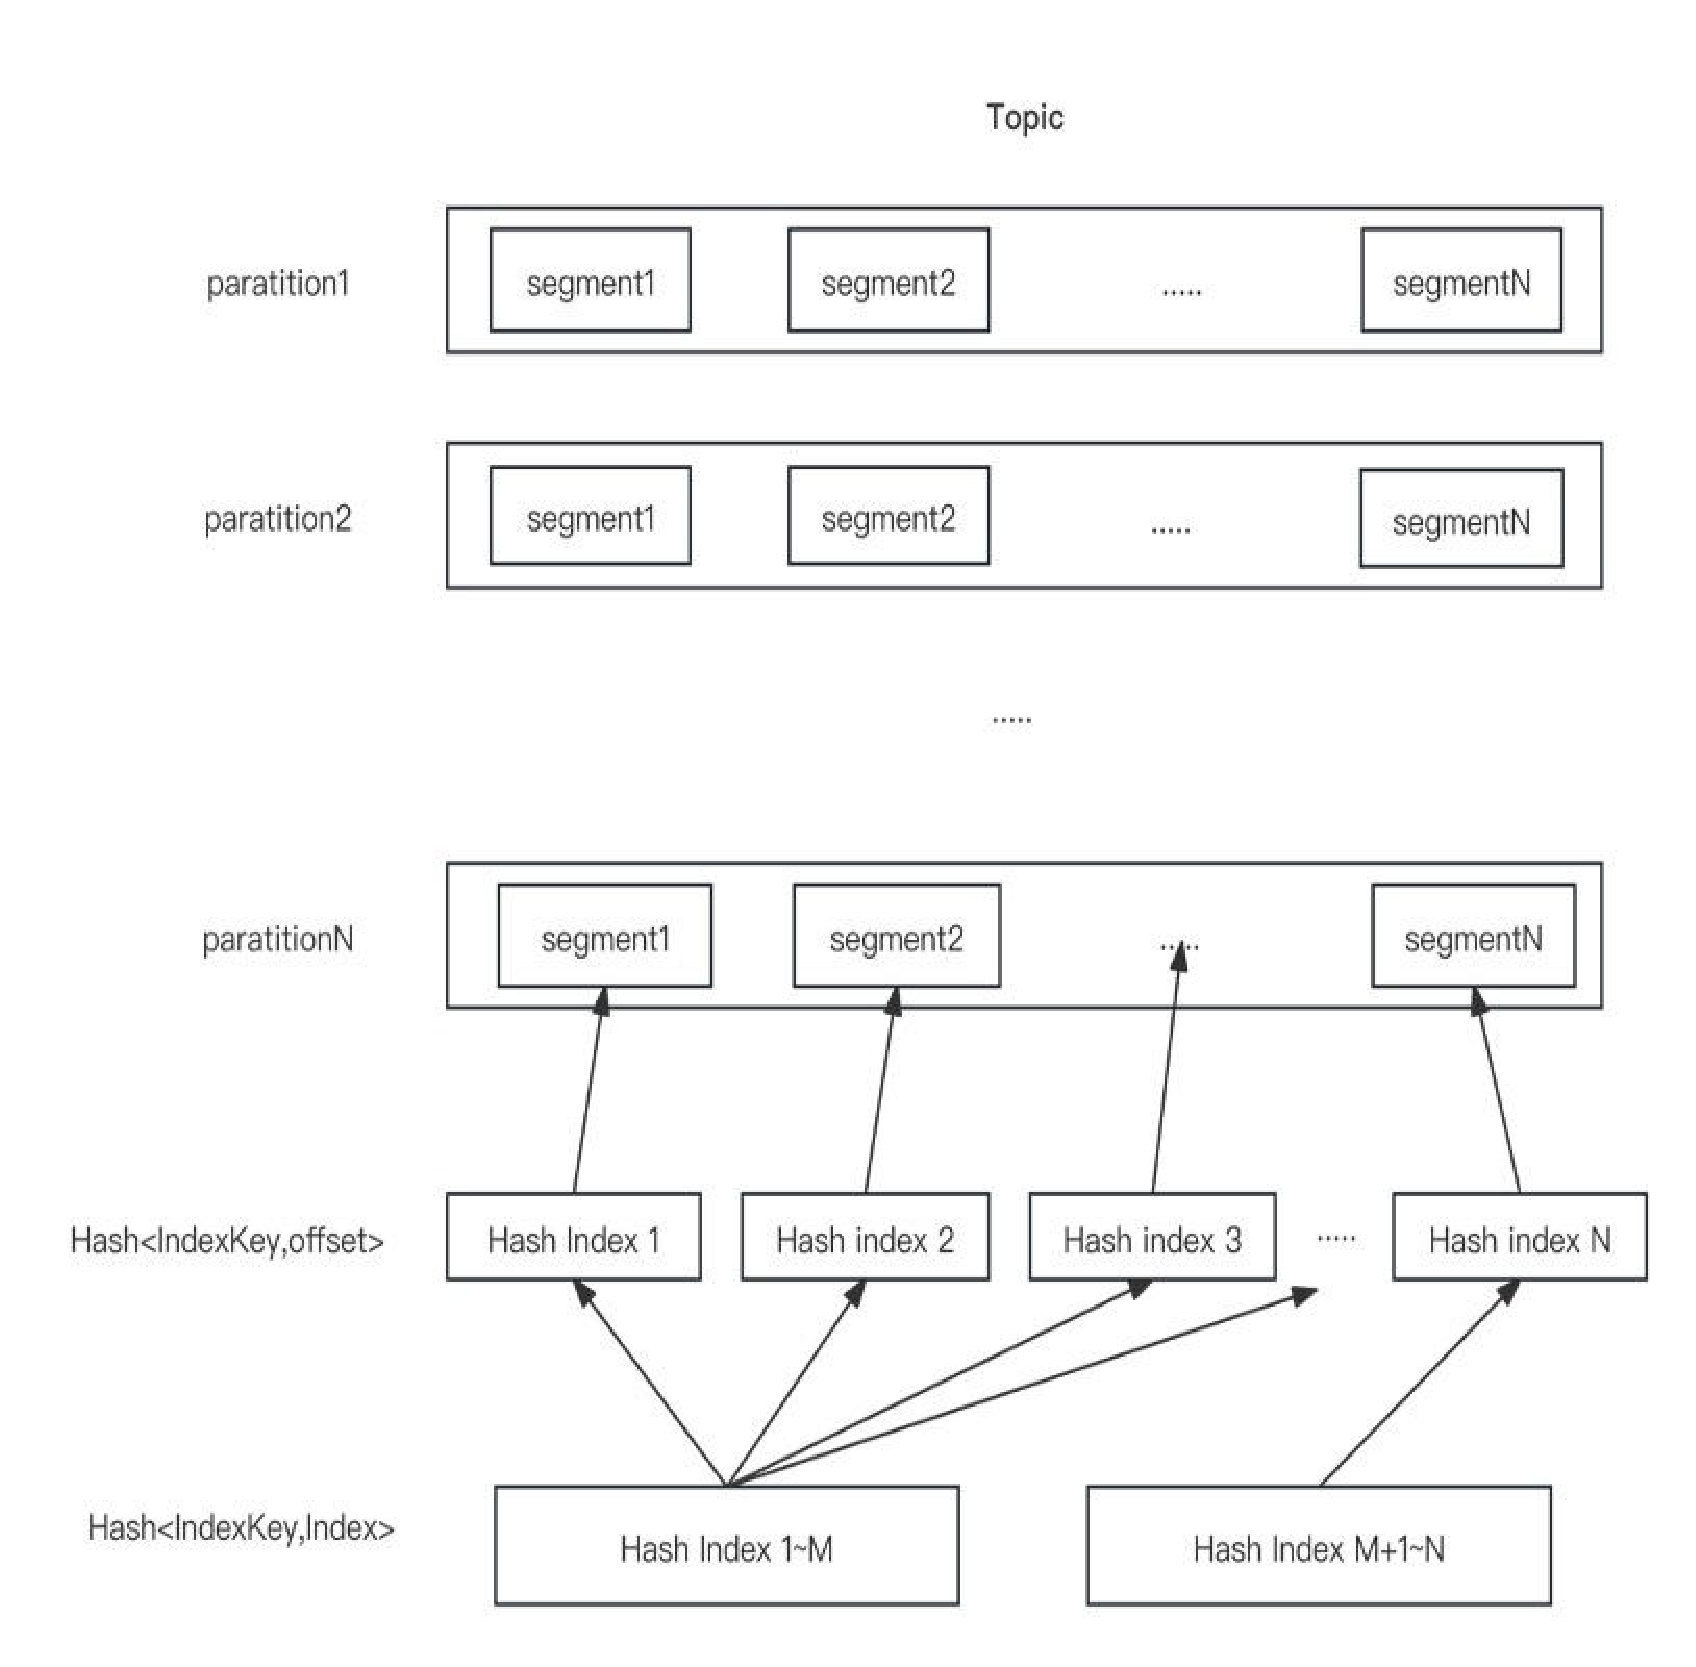
\includegraphics[width=5in]{figure/chapter2/BMQINDEX原理图.pdf}
  \caption{BMQ INDEX原理图}\label{bmqindexyuanli}
\end{figure}
BMQ Index应用场景为写入数据为结构化数据,目前支持JSON和PB格式。写需求远大于读需求。需要对统一个Value做多维索引,即多个IndexKey定位同一个记录。对于同一个IndexKey的数量不要太多,否则会影响查询速度,推荐在1000个以内。避免热点数据,PartitionKey的设计最好不要是热点,否则可能导致单分片下索引建立延迟过高。这也是BMQ INDEX存在的弊端,目前很难做到读写吞吐能力都十分突出。图\ref{bmqindexreadandwrite}展示了BMQ INDEX读写流程:
\begin{figure}[htb]
  \centering
  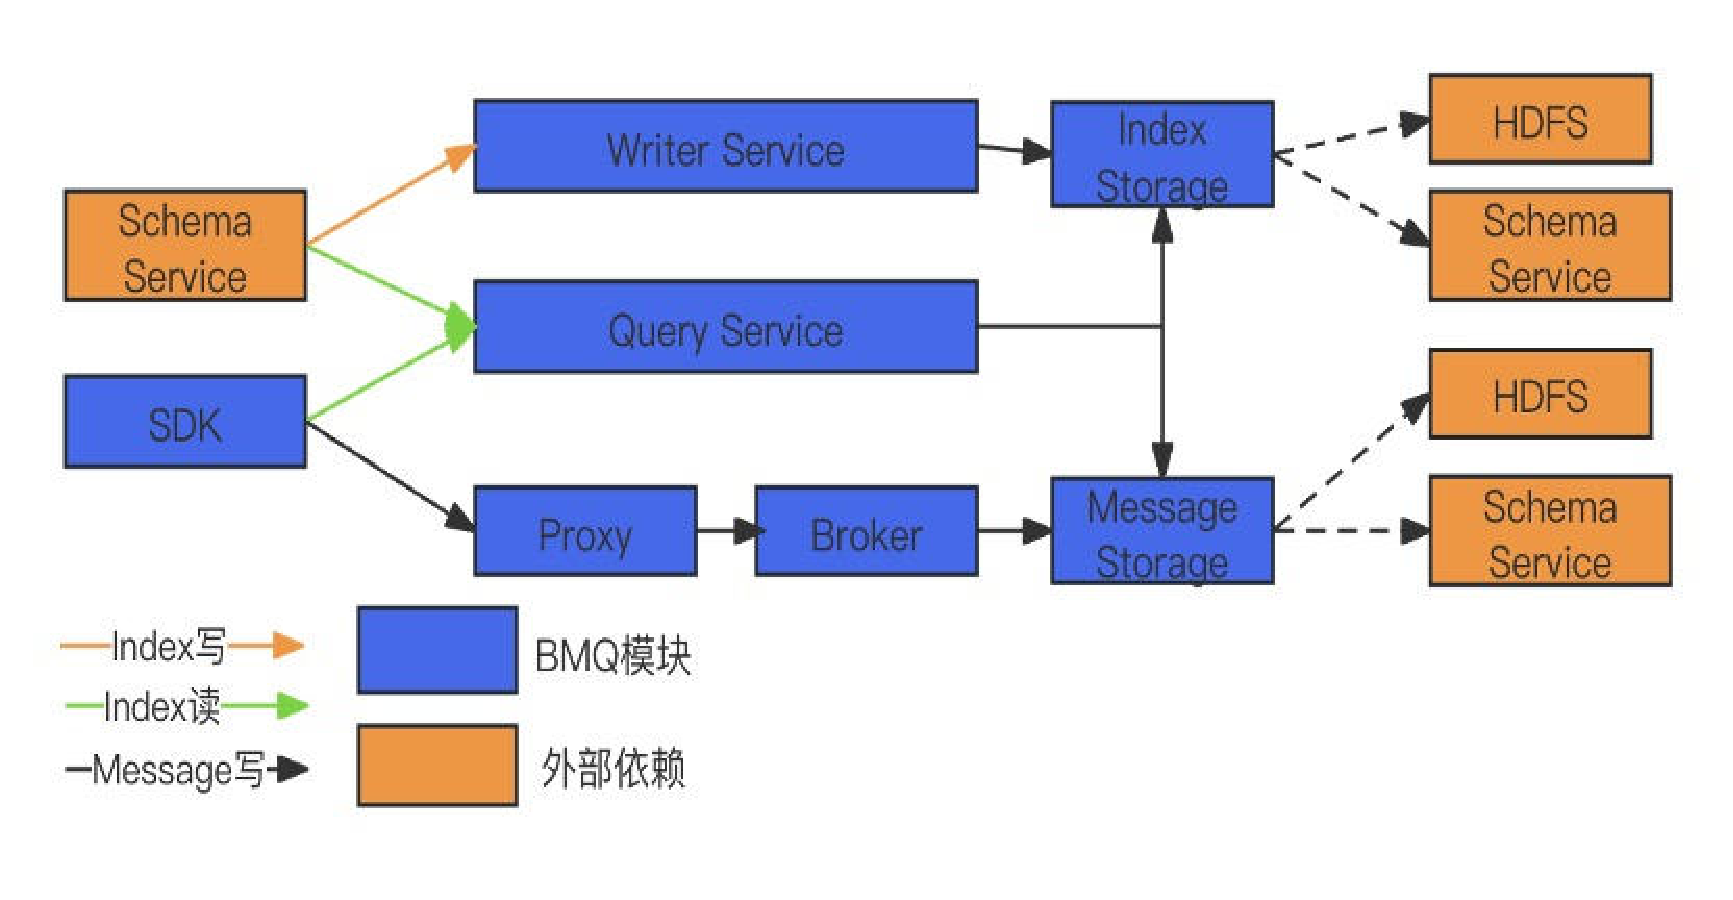
\includegraphics[width=5in]{figure/chapter2/BMQINDEX读写流程.pdf}
  \caption{BMQ INDEX读写流程}\label{bmqindexreadandwrite}
\end{figure}
\section{Kitex} 
KiteX 的目标是实现一个高可靠、高性能、强扩展性、面向开源、业界第一的 Go RPC 框架~\cite{王伟2013rpci}。KiteX 提供了全新的网络库Netpoll,Netpoll是基于Epoll实现的一套新的网络库。自建内存池,提供高性能 Buffer自带流式缓冲区,用户态调用零拷贝,仅在内核态到用户态间执行一次 Copy。Buffer 自增长零拷贝,大包性能优异。使用协程池提供NIO Server,通过 gopkg/gopool 协程池调度和处理任务。框架可以判断正常断开的连接状态,不会获取断开的连接发送请求,避免了Broken Pipe 以及 QPS 较低时长连接反复创建销毁的问题。基于 Netpoll,KiteX 支持了连接多路复用,只需要一个连接就可以完成端对端所有请求,压测中服务端使想啥呢用连接多路复用较连接池场景QPS高出30$\%$。
在Trace系统中包括很多微服务,上下游之间都是通过Kitex进行的远程通信。上下游定义好Thrift文件格式~\cite{田翠珍2016基于},然后借助Kitex脚本文件通过指令的形式自动生成Client和Sever通信交互的代码。图\ref{Kitex}为Kitex的主要结构:
\begin{figure}[htb]
  \centering
  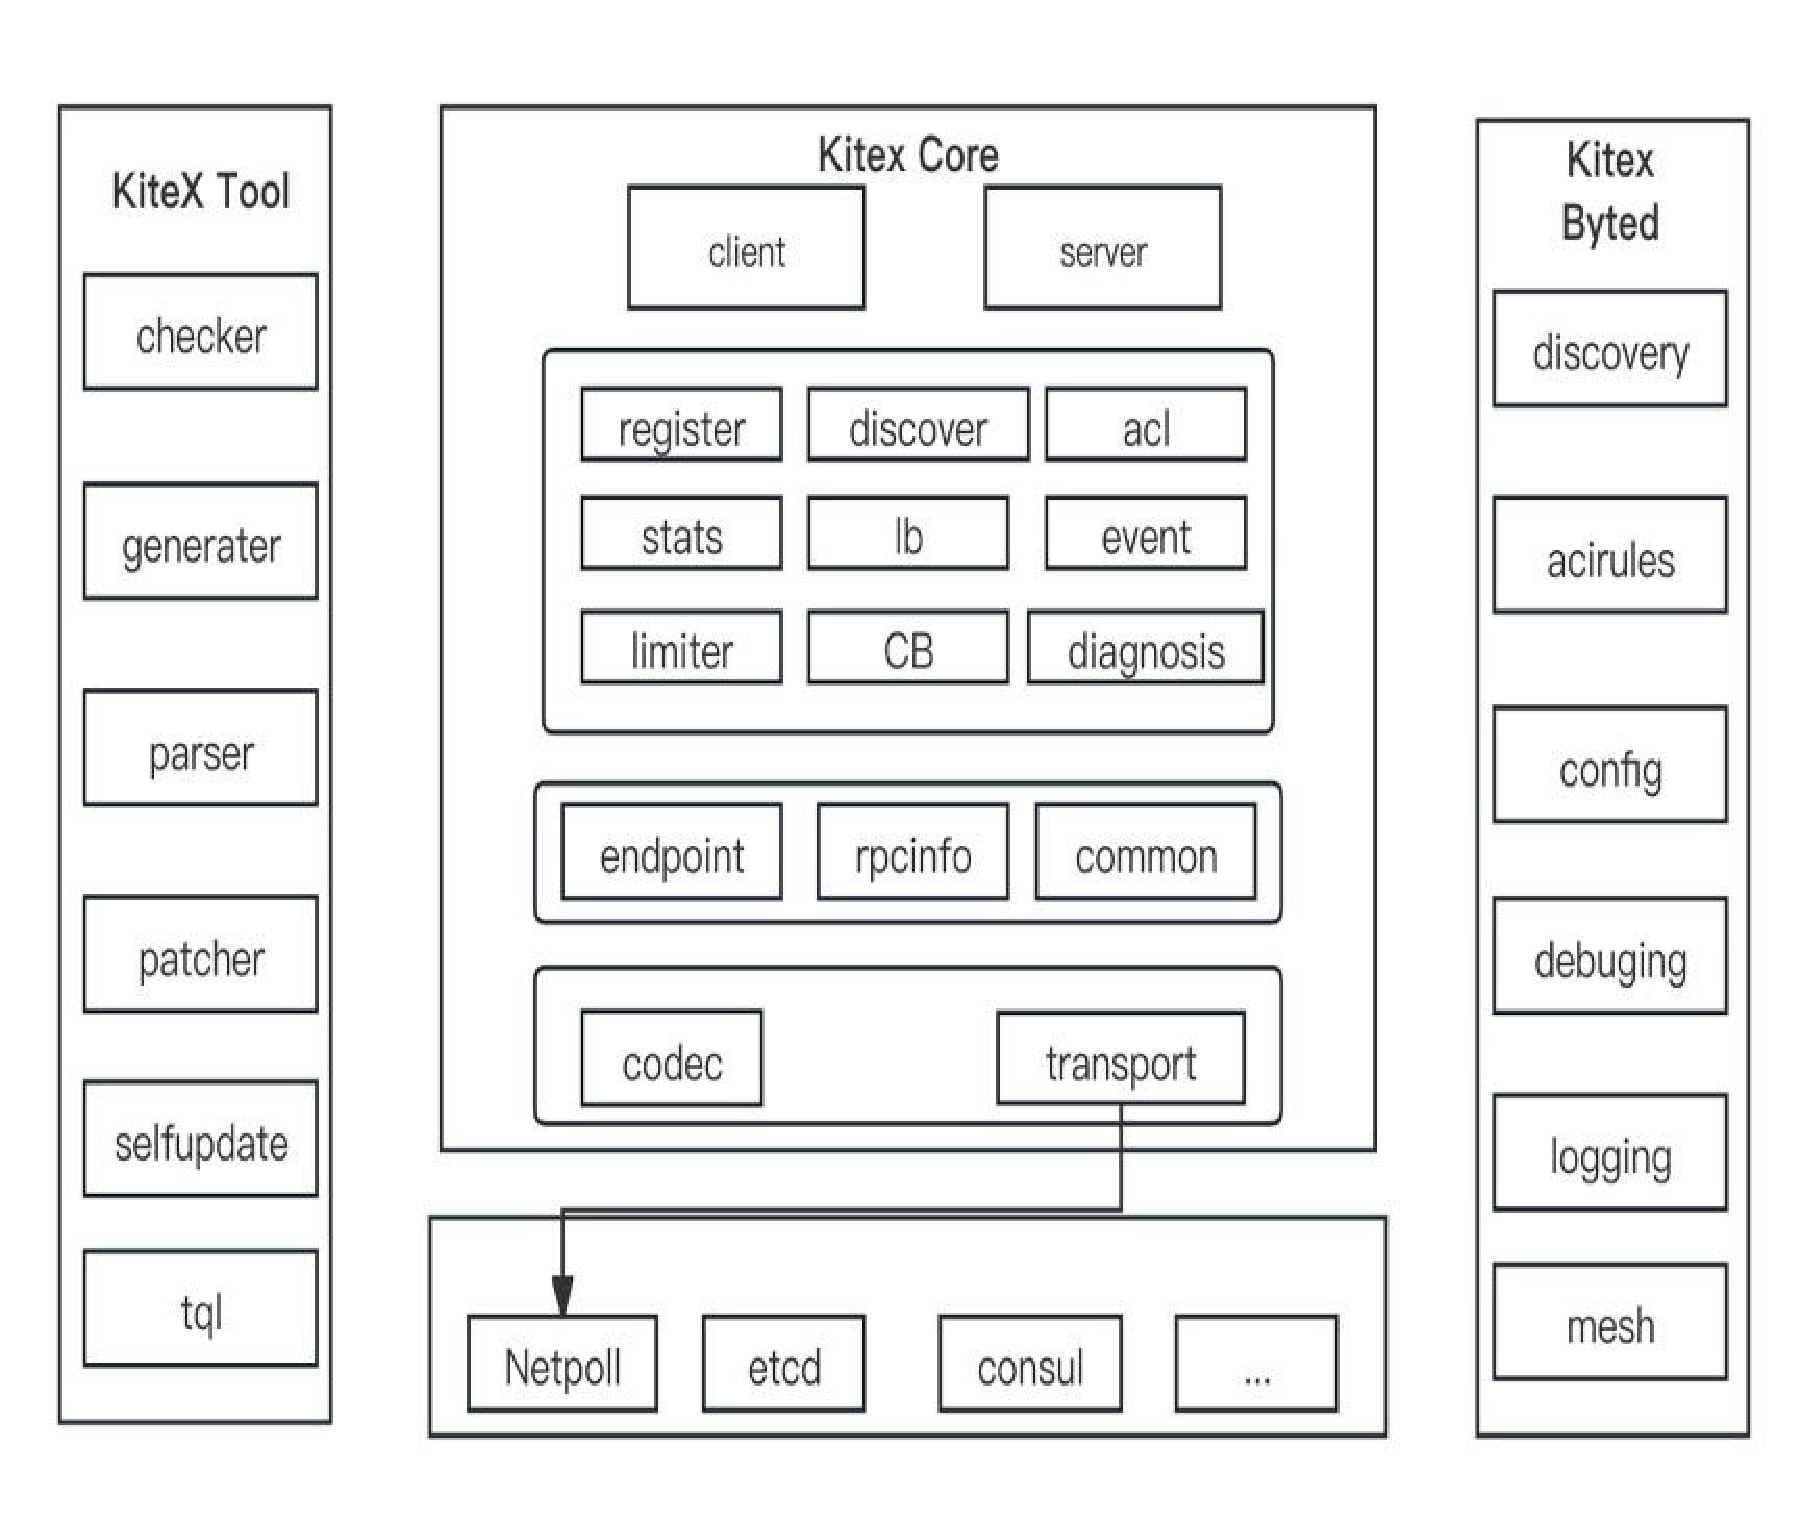
\includegraphics[width=5in]{figure/chapter2/Kitex架构图.pdf}
  \caption{Kitex架构图}\label{Kitex}
\end{figure}
\section{Elasticsearch}  
Elasticsearch 是一个分布式、RESTful 风格的搜索和分析引擎,通常用于处理大量的文本数据。Elasticsearch 是分布式的,意味着它可以在多个机器上运行,并通过网络连接在一起。这使得 Elasticsearch 能够处理大量数据,并在高流量下保持性能。Elasticsearch提供了一个基于RESTful(Representational State Transfer)的 API,可以使用各种语言(如 Java、Python、Ruby)进行交互。所有 Elasticsearch 数据都以 JSON(JavaScript Object Notation)格式存储和交换,这使得数据的处理和传输更加高效和灵活。在 Elasticsearch 中,数据存储在索引中,索引又分为多个文档。文档是 JSON 格式的对象,表示一个单独的数据记录,可以包含多个字段。每个文档都有一个唯一的 ID。Elasticsearch 支持全文搜索、地理位置搜索、多语言支持等高级搜索功能,可以根据数据的内容和属性进行搜索。Elasticsearch 可以对文本数据进行分析,例如词干提取、停用词过滤等,这些分析结果可以用于搜索或其他用途。图\ref{ElasticSearch}为
Trace系统中对Elasticsearch的请求访问:
\begin{figure}[htb]
  \centering
  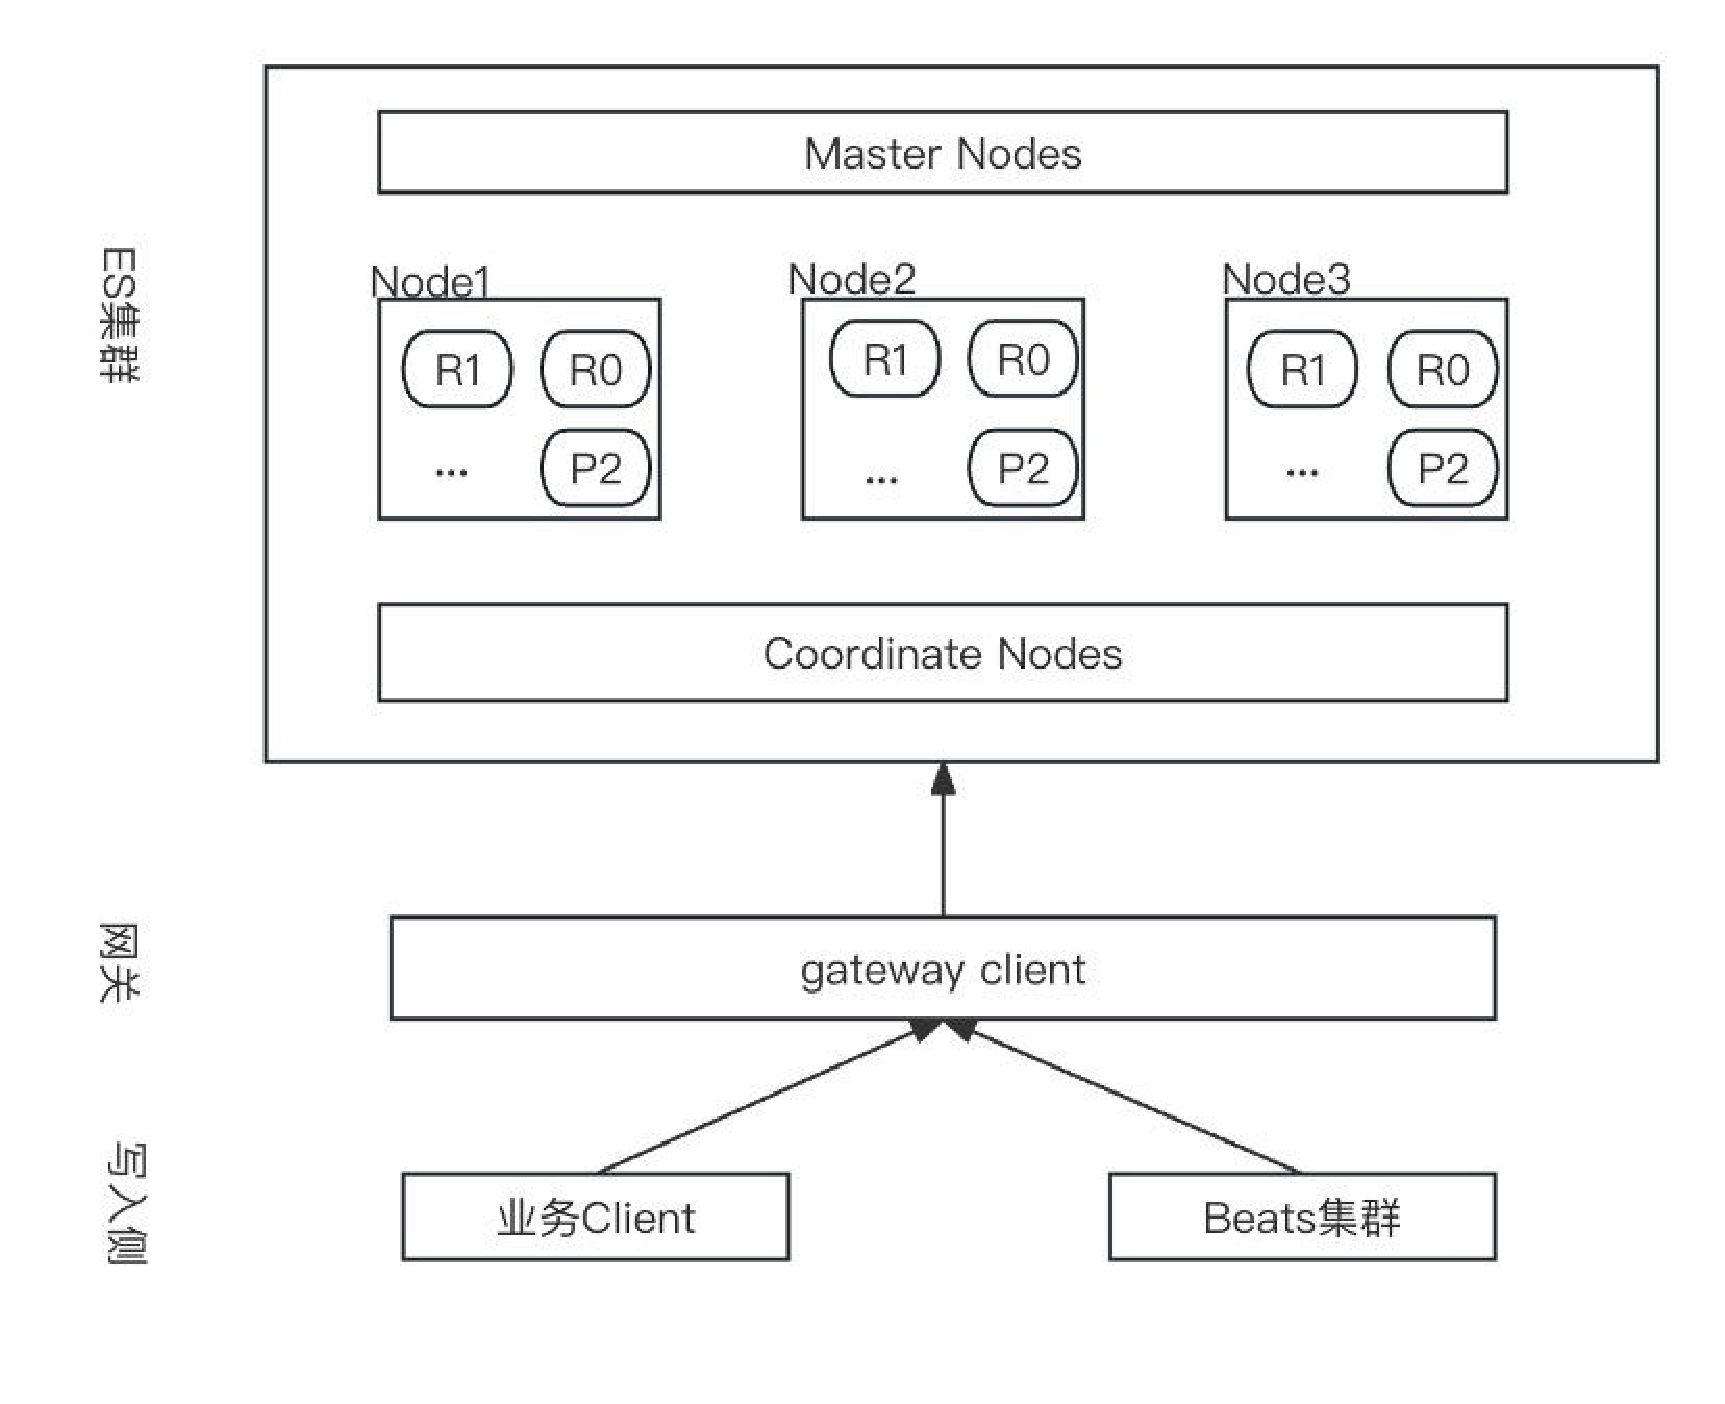
\includegraphics[width=5in]{figure/chapter2/ElasticSearch请求处理结构图.pdf}
  \caption{ElasticSearch请求处理结构图}\label{ElasticSearch}
\end{figure}

在Trace系统中ElasticSearch并没有完全被替代,而是将少量的埋点字段当作索引放在ElasticSearch中。查询首先根据索引字段在ElasticSearch中进行倒排查询,拿到所有符合条件的文档ID,再根据文档ID进行BMQ INDEX的点查,从而获取到记录的全量的数据内容。

ElasticSearch中索引字段具有数量上的限制,可以手动进行配置,比如规定最大的索引字段数为50,多于50将使用LRU算法~\cite{阳慧2004lru}将最近未使用的字段过期掉,那么ElasticSearch必须采用动态索引的方式来适配该功能。将索引字段放入Mysql中进行记录,索引字段的确立可以让用户进行选择,索引过期功能对用户来说是透明的。

\section{Redis}  
Redis 是一种基于内存的数据库,用于存储键值对数据。它支持多种数据类型,包括字符串、列表、哈希表、集合和有序集合等。Redis还可以用来做分布式锁,这得益于Redis作为一个内存数据库,其高性能的特性使其能够在分布式环境中高效地处理锁操作,采用单线程模型,这意味着它可以更好地控制资源的使用和分配,避免了多线程环境下可能出现的复杂性和潜在风险,提供了如`SETNX`和`EXPIRE`等原子操作,这些操作保证了操作的原子性,即要么全部执行成功,要么全部失败,这使得它们非常适合于分布式锁的场景,具备一定的容错能力,即使在部分节点出现问题时,仍然可以通过大多数正常的节点继续提供服务,这对于分布式锁来说是一个重要的优势,Redis还支持Lua脚本,允许用户编写自定义的函数来管理锁,进一步增强了分布式锁的可定制性和安全性。

项目中Redis采用Cluster集群部署模式,采用一致性哈希方便对Redis进行水平扩展,通过增加虚拟节点可以使发生故障的节点进行数据转移达到再平衡,图\ref{redis}详细展示了其原理:
\begin{figure}[htb]
  \centering
  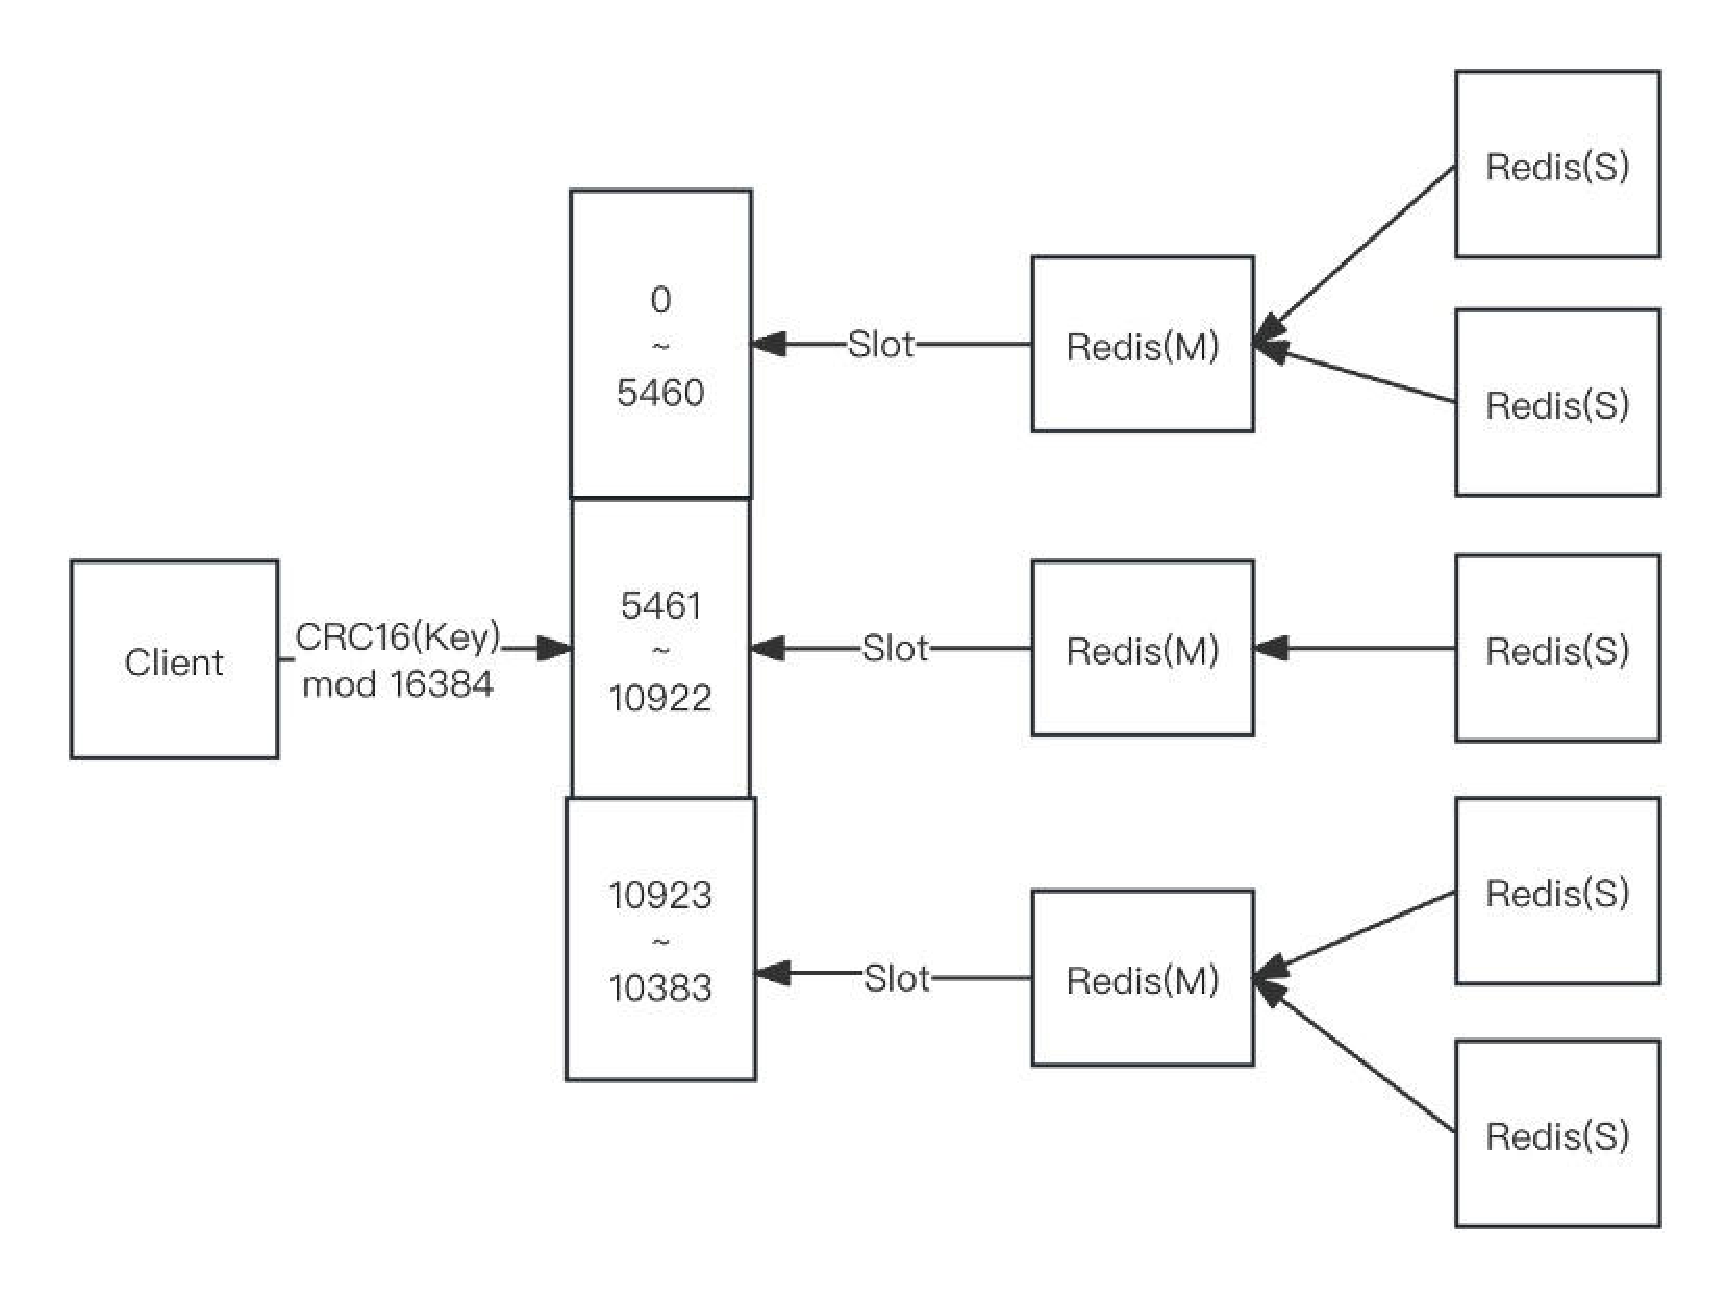
\includegraphics[width=5in]{figure/chapter2/Redis集群架构图.pdf}
  \caption{Redis集群架构图}\label{redis}
\end{figure}

Redis在系统中主要有两个用处。项目要做到集群化部署,LRU算法的字段数据是需要缓存在Redis中的,图~\ref{LRU}详细展示了其原理。在Trace离线查询的时候Redis还会用来做分布式锁,来保证集群化部署时只有一个容器在使用资源。

\begin{figure}[htb]
  \centering
  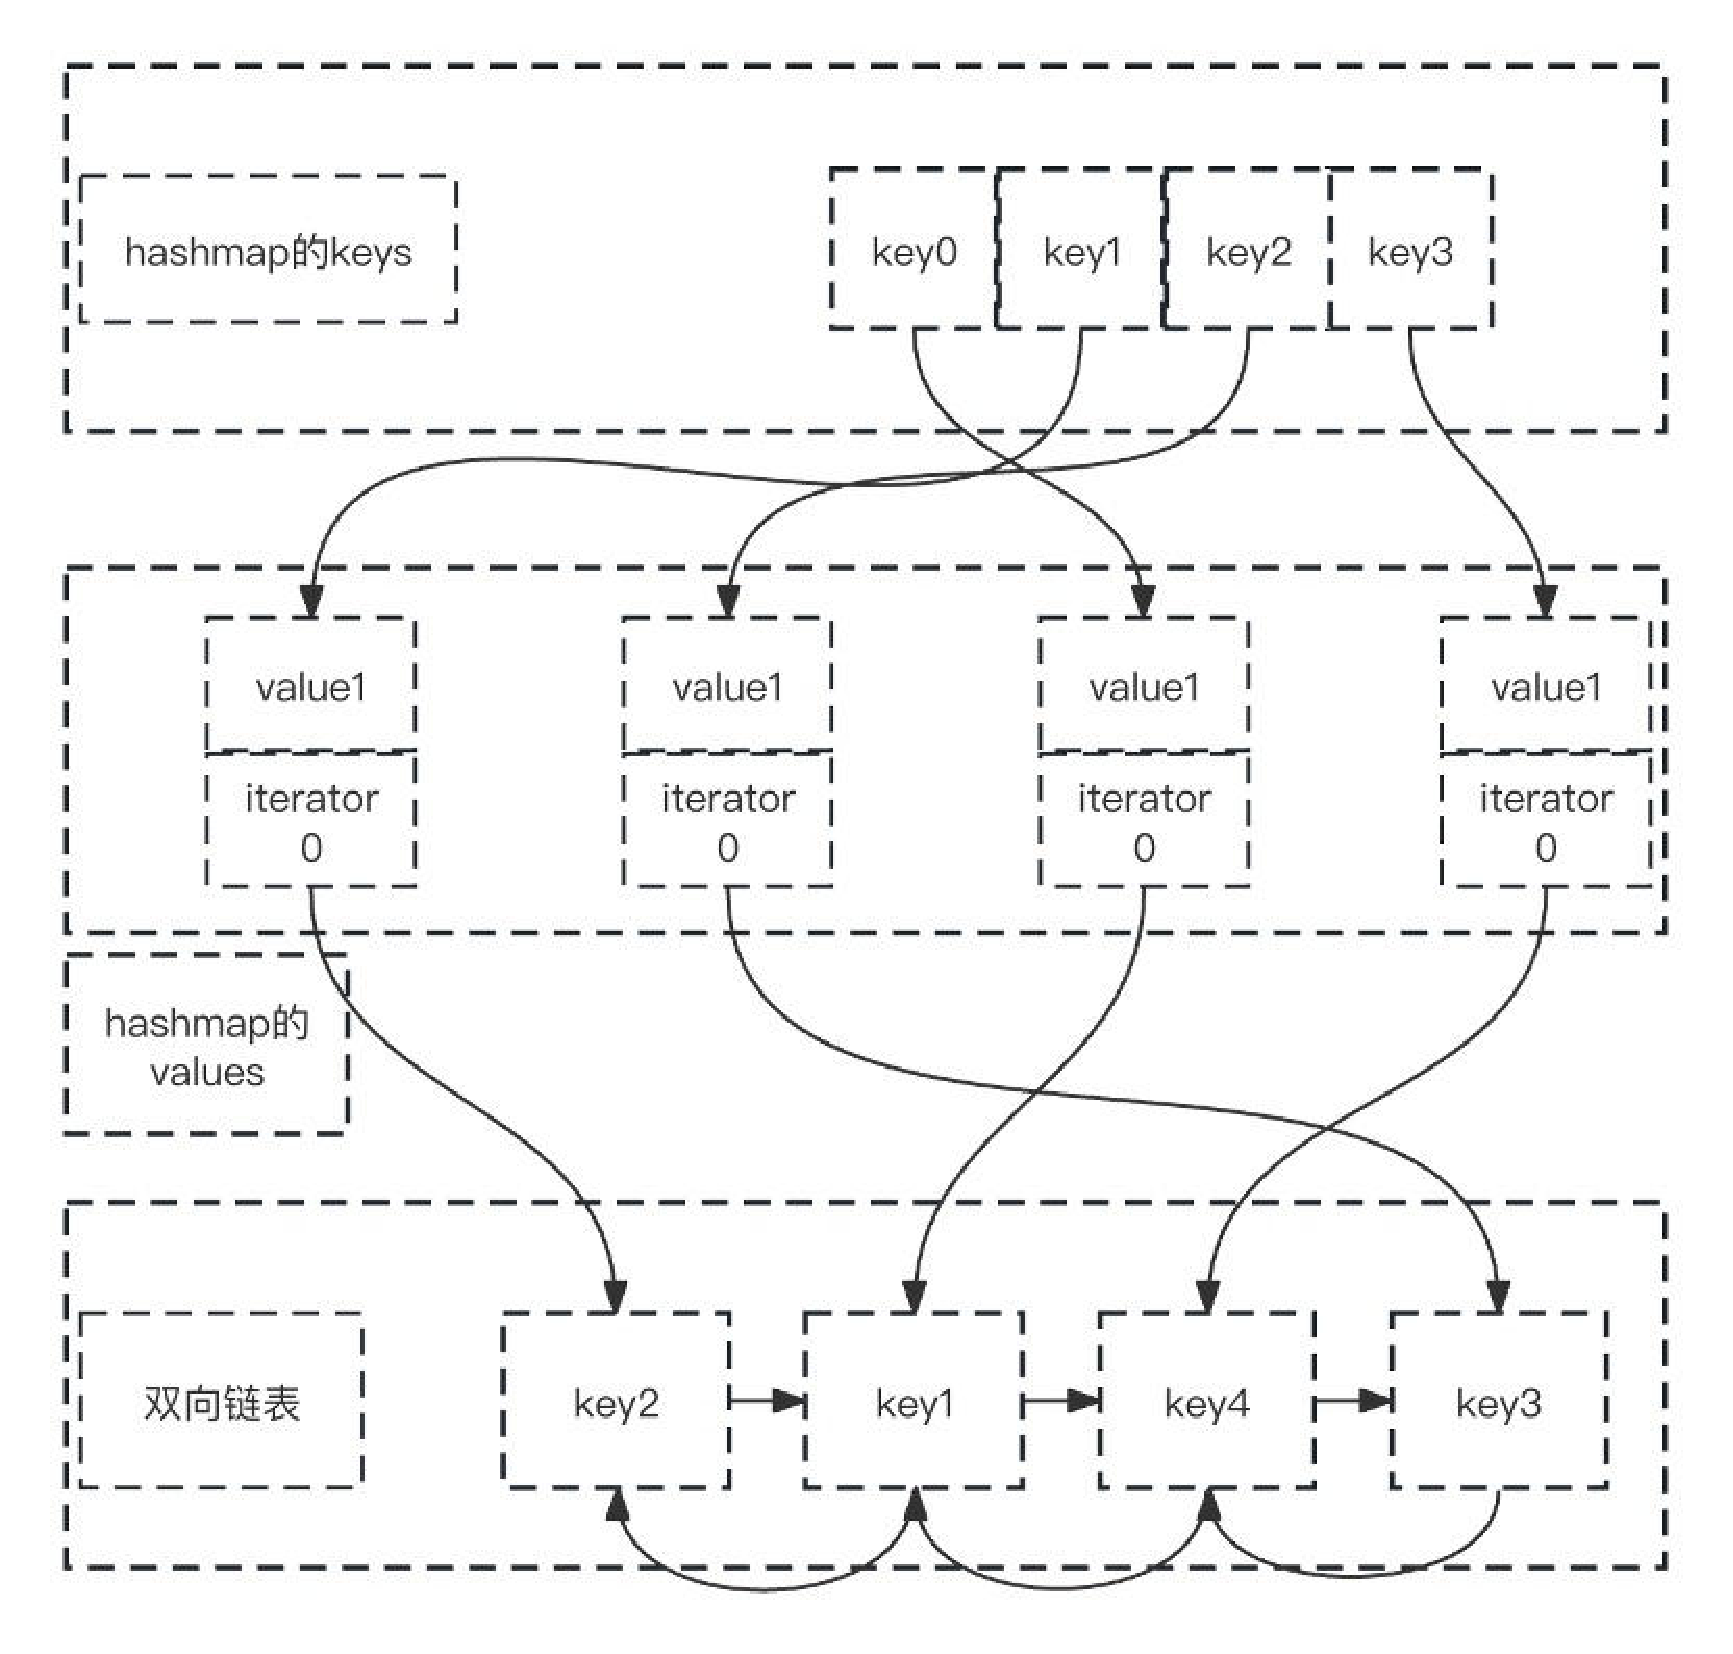
\includegraphics[width=5in]{figure/chapter2/LRU算法原理图.pdf}
  \caption{LRU算法原理图}\label{LRU}
\end{figure}
\section{TCC} 
TCC 全名是“动态配置中心”,可以将一些配置类放到该平台上,并借助该平台发布至CDN。相较于写到代码中,修改配置无需走项目上线流水线的完整流程(拉分支、改代码等),只需要在平台上进行修改和发布,将配置内容与代码解耦,在一个地方统一管理,支持将配置以低代码形式,开放给非开发人员(如产品等)进行修改。

\section{Snappy} 
Trace日志具有数据规模庞大、留存时间长、写入速度快、有用信息密度低、访问延迟要求高等特点。为了节省存储成本,需要满足3个要求:1)以较高压缩密度保存此类数据(压得狠);2)以较高的压缩速度实现数据写入(压得快);3)以低延迟对压缩数据进行快速检索(查得快)~\cite{魏钧宇2023数据模式感知的低成本云日志存储系统},同时实现这三者是充满挑战。看一个压缩算法的优劣,有两个重要的指标:一个指标是压缩比,原先占 100 份空间的东西经压缩之后变成了占 20 份空间,那么压缩比就是5,显然压缩比越高越好;另一个指标就是压缩 / 解压缩吞吐量,比如每秒能压缩或解压缩多少 MB 的数据。同样地,吞吐量也是越高越好。由于Trace系统面向的用户巨大,如果压缩速度不能做到极致,那么经过巨大数据量的并发上报,服务端会产生数据的堆积,这对实时日志检索来说是个灾难性的弊端。下面就常见的压缩算法做一个对比: 

\begin{table}[htb]\footnotesize  
\centering  
\caption{调研压缩算法对比}  
\vspace{2mm}  
\begin{tabular}{lccccc}  
\toprule  
\multirow{2}{*}{\textbf{Format}} & \multicolumn{2}{c}{\textbf{Size (byte)}} & \textbf{Compress} & \textbf{UnCompress} & \multirow{2}{*}{\textbf{MAX CPU}} \\  
 & \textbf{Before} & \textbf{After} & \textbf{Expend(ms)} & \textbf{Expend(ms)} & \textbf{($\%$)} \\  
\midrule  
\textbf{Bzip2} & 35984 & 8677 & 11591 & 2362 & 29.5 \\ \hline  
\textbf{Gzip} & 35984 & 8804 & 2179 & 389 & 26.5 \\ \hline  
\textbf{deflate} & 35984 & 9704 & 680 & 344 & 20.5 \\ \hline  
\textbf{lzo} & 35984 & 13069 & 581 & 230 & 22 \\ \hline  
\textbf{Lz4} & 35984 & 13069 & 581 & 230 & 22 \\ \hline  
\bottomrule  
\end{tabular}  
\label{table:suanfa}  
\end{table}


上表从压缩前后数据量大小、压缩和解压缩吞吐、CPU使用率上进行了对比,可以发现snappy相对其他压缩算法在该场景下具有最佳的性能。
\section{Loghouse}  
Loghouse是一个离线的KV存储方案(Key写Redis、Value写HDFS),适用于 key 小 value 大的写 >> 读场景(log,debug info),主要支持在线的点查询和范围查询。与BMQ INDEX相似也是一种索引存储分离架构。如果单纯使用loghouse 作为存储方案,会存在热key问题,且写入 QPS 会跟随查询维度成倍提升(增加一个查询条件组合就增加一倍的QPS),意味着 Redis的成本也会倍增,故不适合用于查询条件丰富的场景。loghouse服务的价格相对来说比较昂贵,对于iops很高的请求,对Redis的qps也会很高,并且Redis基于qps来收费,Redis的成本也会很高。
\section{小结}  
本章阐述了构建超大数据量下埋点字段管理查询系统所涉及到的重点技术介绍,该系统的存储方案最终选取的是BMQ对数据进行存储,这也是比较新颖的地方,传统的消息队列一般用来做流量削峰、异步处理、业务解耦,而这里的消息队列基于HDFS对数据进行存储,并且对写入的数据也不断异步生成索引,从而满足了写吞吐量和查询速度。当然,如果存在热点Key,单独使用BMQ INDEX来进行存储会是个灾难。这里我们仅使用BMQ INDEX作为全量数据存储的工具,因为有Elasticsearch的前置索引存储,这里不用考虑复杂的索引条件,采用 partitionKey和clusteringKey的设计能唯一确定一个打点,也避免了热 key 问题。数据的获取是通过Kitex RPC调用实现的,通过Snappy压缩存储降低了MQ生产和消费的数据规模,从而减少了早高峰数据堆积的延迟,使得查询的时效性得到保障。

\chapter{埋点字段管理查询系统需求分析}
随着抖音APP下载量越来越多和人们花费更多的时间在上面,抖音所产生的日志流变得愈发庞大,想一想全球的用户一秒所产生的日志数据量就达到20G。在生产环境,点播业务每日产生的日志大小约在300TB左右,直播业务的数据集则超过了2PB。那么这些数据如何更好的利用起来成为一个问题。现阶段的全量日志往往包含几百个字段,覆盖各种工程模块的埋点信息。实际场景下,用户往往只关心自己当前开发的,工程模块A相关的埋点信息,对工程模块B/C/etc相关的信息,往往不会同时关心。用户真实关心的日志,和返回数据集相比很小,也就是说该平台提供的不是指标汇总,是明细信息。用户使用平台的目的,是希望查到一到两条关键的明细日志,从而定位开发问题。基本地,维护一套日志ETL工具,肯定是以日志丢失率越低越好,用户查询端到端时延越低越好为目标。

由于平台主要功能是追踪溯源,因此这里就以Trace系统简称。Trace的服务主要对象是研发。因为Trace平台的本质是解决事情发生没有,什么时候发生,如何发生的等信息的查询。Trace消息的收集深入链路内部,基础的Trace消息只有研发理解,收集的信息由研发确定,目的是帮助研发高效的排查当前场景的历史事件信息。在推广的时候,会遇到一些业务方反馈说,这个场景如果接入Trace,东西做出来不是给研发用的,是为了给客服、运营、QA用的。这个当然是可以理解的,但是这个工具的本质还是为研发服务的,因为如果没有这个工具,这些排查工作就会穿透到研发这里来,Trace平台的使用方聚合数据,屏蔽细节,简化操作,是为了尽可能减少这种排查需求穿透对研发的打扰,但是当一些常规排查无法确定时,这部分排查必定会穿透到研发,这时Trace也可以提供更多细节给研发辅助排查问题。从这个角度来看,归根结底,这个平台的服务对象就是研发。

拿字节跳动的直播业务来说,直播Trace平台是面向直播业务,辅助业务团队定位、诊断线上业务异常的的运维平台,并在此基础上拓展了问题发现和恢复的能力。能够帮助业务团队在开发,联调,上线,问题反馈,事故恢复的全流程中提高产品质量,降低事故风险和影响时长,提高人效降低成本。直播Trace能力上主要包括Trace历史记录追溯,业务校验,直播诊断工具等涵盖了从问题发现到解决的全过程。那么Trace到底追求通用还是高效呢?

首先为什么会把这两个对立起来?作为一个想要推广的平台,这关系到之后的开发和接入方式。因为通用和高效在一定程度上,至少在平台发展初期时是矛盾的,一套系统,一个标准必然是最简单通用的,但是定制化会带来更高的使用体验,但是在效率上就会带来损失,目前一套标准至少会带来无法覆盖直播的所有场景,部分场景只能凑活着用。还有就是忽视了业务线之间的区别,妥协导致的接入和理解成本上升。并且一套展示系统带来的查询效率不高,无法覆盖不同场景,不同的业务杂糅,互相干扰,稳定性低,安全性差。其实,业务方也更关注效率,业务方接入SDK,引入了复杂性和不确定性,占用了资源,需要有超出预期的收益。只有高效的解决这个问题才能减少接入阻力,赢得口碑,才能进一步扩展接入场景。通用和效率可以在数据收集和展示方案上做抽象,降低方案的使用成本来提高效率。

基于上述原则和理念,本文提出Trace系统的功能总体可以拆分为四部分,数据的收集,处理和展示以及数据挖掘。这四部分的解决方案都是以超大数据量为前提。数据的收集统一采用SDK收集的方案,但是在设计上考虑采用直接的函数参数指定的模式,也就是针对不同的场景,采用不同的收集函数,SDK对外只暴露统一的初始化和收集函数,这样可以做到用户理解成本低,贴近场景,而且可以限制接入数据,保证之后数据处理和展示的数据合法性。数据的处理主要包括存储前的处理和展示时的处理。存储前主要包括数据的处理,例如数据打平,数据解压缩,数据自动化解析等,目标是业务方可以尽可能的简单的传递参数,而将大多数数据自动化的处理和收集,屏蔽这部分逻辑,此外也会针对部分场景做一些数据的预处理,方便数据的展示。存储后处理主要是数据的聚合,排序,合并等等,得出展示用的数据,为了避免查询超时,这部分逻辑应该尽可能的简单。由于不同的业务对于数据需要了解的信息是不同的,因此通过不同方案的数据展示能极大的提高部分问题的排查效率。目前已经探索的展示方式包括按照时间顺序的事件展示、单次事件的调用链路分析、多层级打点信息聚合。相信在直播业务内这类需求是类似的,当收集足够多的场景,这个可以足够快速复用到其他平台上。

作为一个超大数据量下流媒体数据ELK系统应在通用性和高效之间追求平衡,保障占用了资源,有超出预期成本的收益,并且类似的业务场景可以尝试复用该系统架构实现降本增效。系统以字节跳动直播和点播业务为背景,从数据收集、数据处理、数据存储、数据检索、数据挖掘角度对系统进行设计。数据收集方式可以分为客户端主动上报和服务端定时拉取,主动上报是指客户端APP可以通过SDK将埋点数据上报到数据中心,定时拉取是指可以提供一个工具去定时拉取数据进行融合。数据处理是指对数据进行加工、过滤、清洗,打平,平台应提供定制化的规则来为用户使用。数据存储应与传统ELK系统相比做到降本增效。数据检索要保障实时性和高可用性,为此平台应提供实时查询和离线查询双重保障。告警平台模块是一个指标监控告警平台,致力于提供一站式的指标配置、数据监控和告警推送服务。应实现了基于数据源字段指标的实时或定时的数据采样,并根据不同的检测算法输出告警结果。

通过使用该系统,研发人员、运维人员能够实现对数据的收集、校验、自定义处理规则、自动进行监控报警一体化能力。节约存储成本的同时能够提高定位问题的能力,相对于传统ELK系统功能定制化和自动化,低成本高收益,对于中小型企业需要超大数据量的数据管理可以尽可能实现低投入高回报的效果。

\section{总体规划}
埋点字段管理查询系统的需求描述来源于研发人员,因为大量的非研发人员不能发现问题的本质,只能发起oncall来咨询研发人员。系统主要的功能将新建立的数据源经过数据清洗后存储,提供检索能力和数据自动化监控报警。系统应具备通用性的特征,实现规则自定义化,最终实现降低研发人员oncall压力和提高问题定位能力的目标。
\section{系统功能性需求分析}
在充分分析了上述愿景及总体规划后,系统的功能性需求被划分为4个模块:数据收集模块,数据处理模块,数据检索模块,告警平台模块。本文将结合敏捷开发框架及规范,对每个模块需要处理的任务场景以用例图的方式进行描述,并对每个用例进行详细描述。
\subsection{数据收集模块需求分析}
数据处理模块的用例图如图\ref{dataColl}所示:
\begin{figure}[htb]
  \centering
  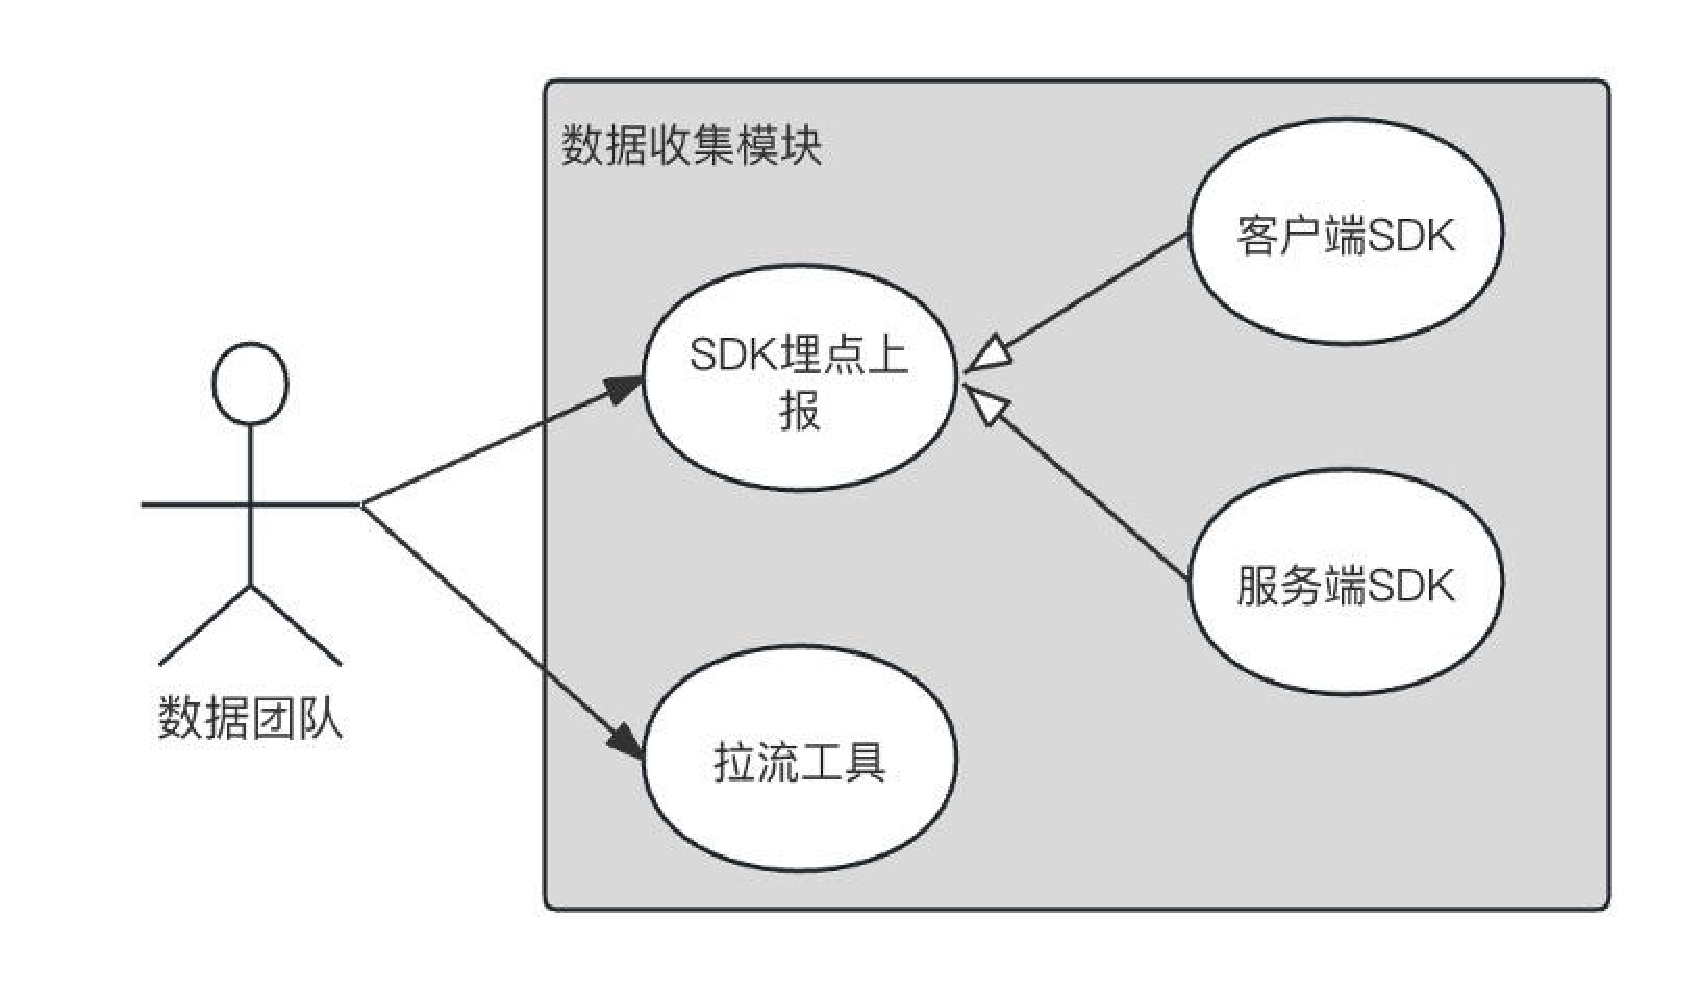
\includegraphics[width=5in]{figure/chapter3/数据收集模块用例图.pdf}
  \caption{数据收集模块用例图}\label{dataColl}
\end{figure}
 
SDK埋点上报工具~\cite{张永勐2022基于用户大数据分析的物联网家电质量改善方法研究}就是可以内置在代码中的软件工具包,可以将内置在APP客户端和服务端中,可以使用它去做各种数据的采集和上报,统一上报到数据团队的清洗服务器做数据处理。如果涉及到的功能、模块和部门非常多,数据处理团队如何去处理接收到的海量数据?那么就需预先规定好日志上报格式和日志的消费流程。日志上报的内容都是Key-Value形式的,但是不同来源的日志上报的方式不同,需要通过内容中的特殊的字段来标识。但是事件之间如果没有关联,很难用于产品分析。每个状态下会有唯一的SessionId,用SessionId将事件串联起来。数据不加密进行上传会影响用户信任度,存在泄露风险,可能引发严重的品牌和政策风险。上报数据应进行压缩,提升后端吞吐量,从而提升上报成功率。某些活动场景数据上传会面临巨大的服务端带宽压力,为了避免负载超载情况下拥塞加剧,需要数据收集SDK进行主动避让,降低上传间隔。

拉流工具是调用远程数据服务接口,定时拉取并处理存储数据中心。核心模块为数据拉取,数据处理,数据导出三个模块。数据拉取模块首先应具有拉取接口的Token,构造符合接口要求的请求并拉取数据,数据处理模块从拉取的数据中提取所需要的字段,检查处理后的数据格式,数据导出模块根据配置将处理后的数据存储。

\subsection{数据处理模块需求分析}

该模块的功能性需求包括四个用例:数据加工用例、数据过滤用例、数据清洗用例、数据打平用例~\cite{严霄凤2013大数据研究}。涉众为数据团队人员,即在对数据进行使用前需要对数据进行处理的数仓团队。
\begin{figure}[htb]
  \centering
  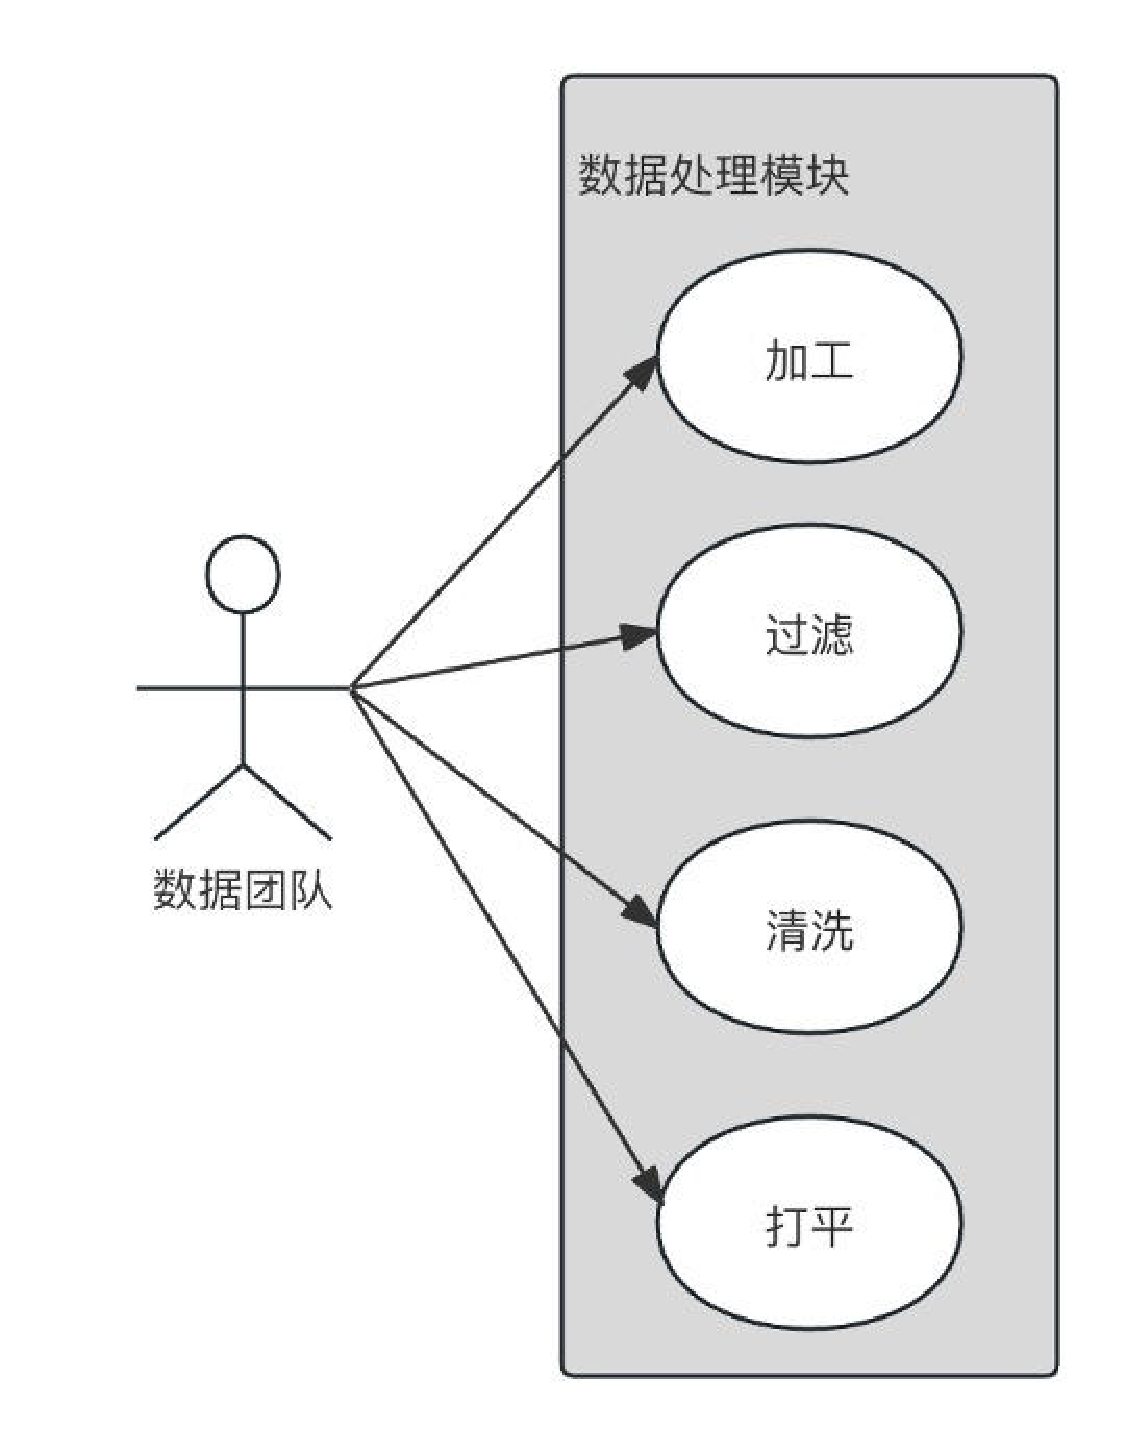
\includegraphics[width=5in]{figure/chapter3/数据处理模块用例图.pdf}
  \caption{数据处理模块用例图}\label{dataColl}
\end{figure}

每个数据源下可以定义多个加工任务,多个加工规则,每个加工任务可以绑定多个加工规则。加工规则只有被加工任务绑定并启动才能生效。从资源成本的角度考虑,每个数据源下应当只定义一个加工任务,通过绑定多个加工规则实现不同的加工转发效果。新建加工规则需要定义上下游信息和具体过滤规则。上下游信息是控制下游 MQ 类型、写入的Topic、Cluster。

过滤规则分为筛选条件和清洗规则。Schema 表示业务方注册上报的字段信息,用于实现业务数据字段级别的写入过滤,未注册的字段上报时将被丢弃;支持JSON打平,可以获取JSON串下的某个字段。支持 >= ,=<,<,>,==,!=,in,not in,pre(前缀),suf(后缀)的筛选过滤;判断字段值 in,not in数组列表中。数据清洗包括检查数据一致性,处理无效值和缺失值等,用户提前设定根据某些字段进行清洗。

数据打平是指将不同层次、不同结构、不同格式的数据进行统一处理后转化为相同的数据格式并用于数据分析和处理。旨在消除数据混乱和不兼容的问题,最终得到结构字段一致的数据进行存储。

\subsection{数据检索需求分析}
数据检索模块的用例图如图\ref{datachuli}所示,该模块的功能性需求包括两个用例:数据检索和字段管理。涉众为查询定位问题的用户,可以是研发人员和非研发人员等需要对问题进行定位分析的人员。
\begin{figure}[htb]
  \centering
  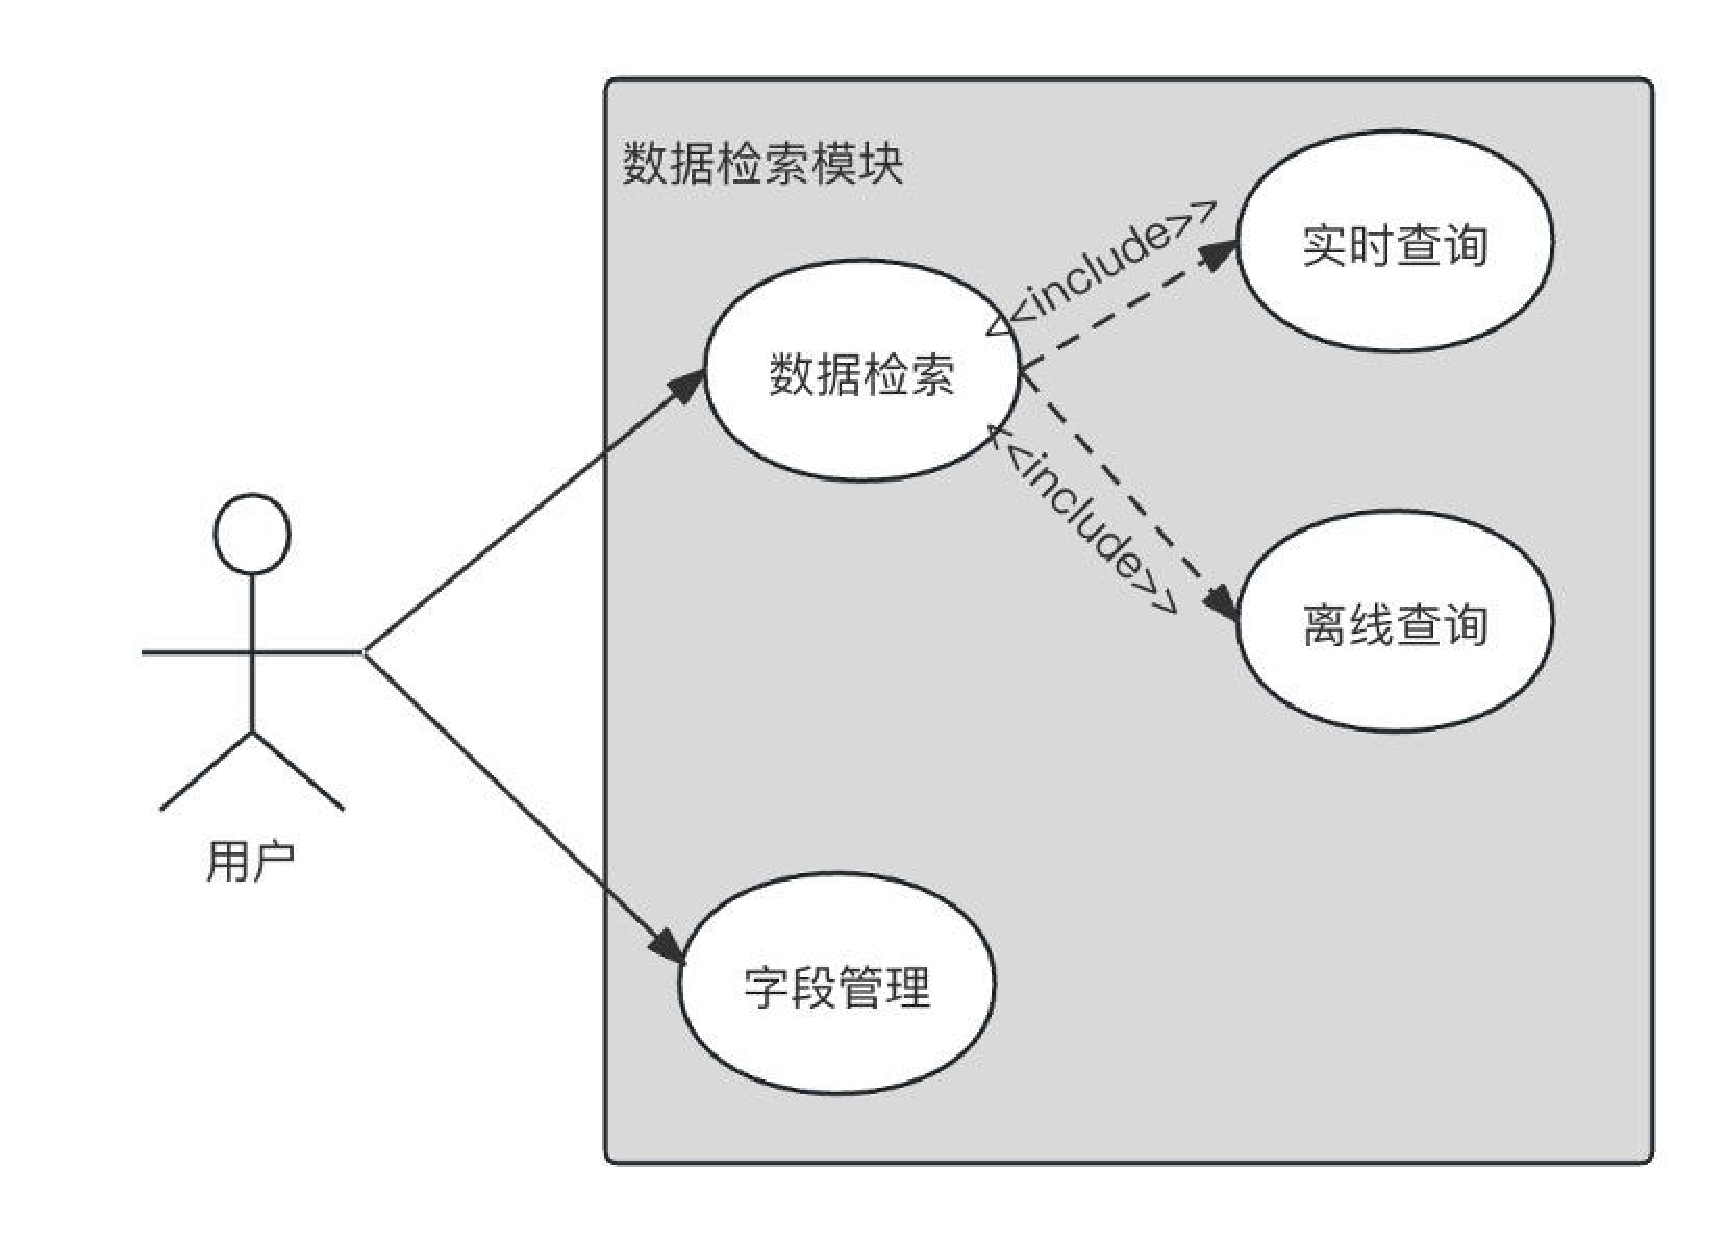
\includegraphics[width=5in]{figure/chapter3/数据检索用例图.pdf}
  \caption{数据检索用例图}\label{datachuli}
\end{figure}

实时查询就是能够在可控的时间范围内返回查询结果,使用户可以快速进行定位分析,如果返回的结构集十分巨大,并且系统之间是通过RPC进行信息的传递,往往会在传递数据时出现服务TimeOut造成本次查询失败。并且实时查询的数据一般保存的TTL都比较短,这个时候难道就没办法进行问题的定位分析了吗?因此,又提供了离线查询方式。所谓离线查询是通过离线批处理任务进行查询,响应结果的时间是不可控的,多则一天,少则几秒就可以完成,并且数据的保留时间很长,在实时查询数据过期和查询失败时,离线查询无疑是一个好的兜底。
    
对于用户来说,不管是实时查询和离线查询最终都是展现准确的结果,尽管这两种查询方式的底层数据流逻辑千差万别,但是最终的表现结果应在同一个前端界面进行展示,应做到对用户透明。并且提供筛选条件供用户进行选择,以便后端进行数据过滤。

用户使用该系统的目的是希望查到一到两条关键的明细日志,从而定位开发问题用户往往只关心自己当前开发的,工程模块A相关的埋点信息,对工程模块B/C/etc相关的信息,往往不会同时关心。因此字段管理在该场景下尤为重要。


\subsection{告警平台模块需求分析}
该模块的功能性需求包括四个用例:告警基本配置、告警指标配置、告警检测配置、告警接收配置。
告警基本配置是指对该告警记录的配置,具有唯一标识该告警任务的ID、以业务背景命名的名称、对告警的详细描述、发生告警时通知的用户等元数据。 

告警指标配置是对数据源字段指标的配置,选取指标相应维度,填写检测维度取值,设置好指标数据拉取的时间窗口,采样的数据作为后台检测算法的输入,设置好采样指标数据的聚合粒度(时间GroupBy区间长度)。

检测配置为配置好检测频率和检测算法,检测算法分为静态阈值算法和同比算法。静态阈值算法配置项有大于(>)、小于(<)、大于或等于(>=)、小于或等于(<=)某个值。而同比算法配置的参数值是是波动值,比如配置了0.1,代表波动10$\%$。当前周期的数据和昨天同周期以及上周同周期的数据进行对比,波动超过配置的参数值就进行报警。系统发现异常后,会向用户发送通知告警图表,并通知相关告警接收人。通知中的曲线无论异常时间长短,都按照自然日进行展示。如果告警已经在处理了,为了防止连续收到告警,可以点击按钮屏蔽告警一段时间,该屏蔽只针对这个告警配置生效,不会影响其它的告警,业务恢复正常后,点击“取消屏蔽”恢复正常告警。告警平台模块用例图如图\ref{gaojing}所示:

\begin{figure}[htb]
  \centering
  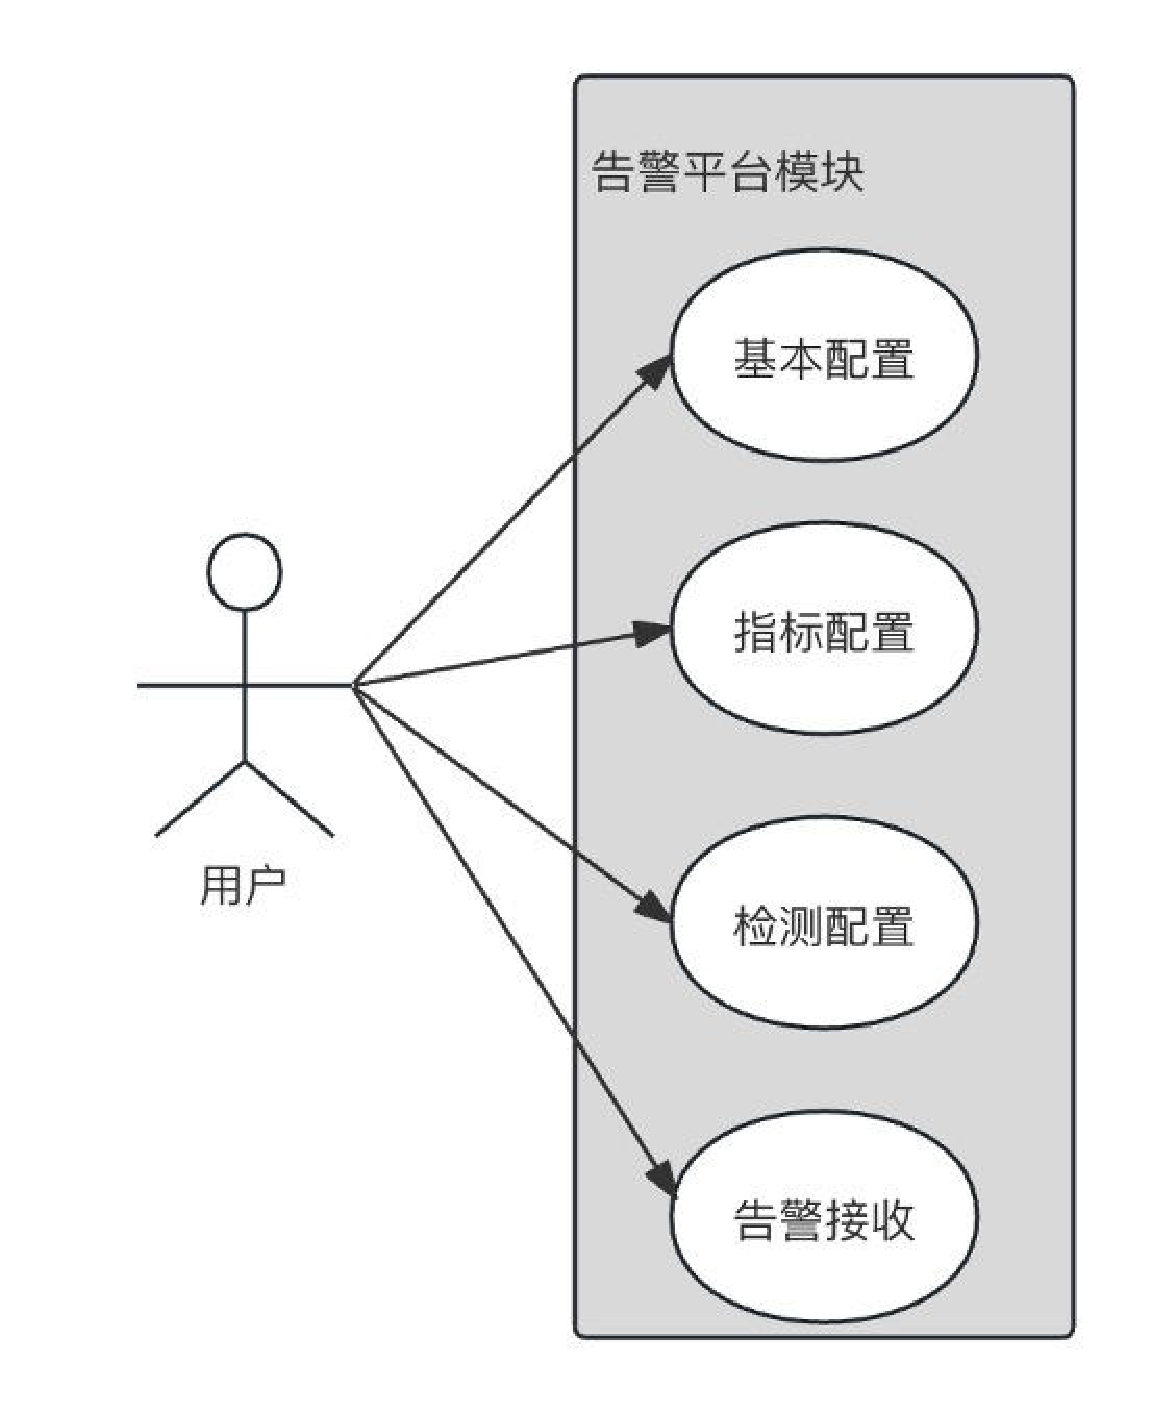
\includegraphics[width=5in]{figure/chapter3/告警平台模块用例图.pdf}
  \caption{告警平台模块用例图}\label{gaojing}
\end{figure}

\section{系统非功能性需求分析}

结合项目要解决的问题及应用场景,该系统需要满足四点非功能性需求:

性能:本系统作为大数据量下的数据点查系统,实时查询时间响应时间应尽可能的快,应保证5秒内作出响应;由于数据流并发量巨大,消息队列数据堆积Lag应保证在可控时间段内;日志上报以后应在10秒内就可以被实时查询到;

安全性~\cite{王伟2013rpci}:系统应该仅允许经过验证的、且被授权的用户进行使用;应该对各种类型的用户授予不同的权限控制,保障系统的安全性,数据传输中不丢失,充分保障通信秘密性。

可扩展性~\cite{寇雅楠2003基于}:考虑到用户刷抖音的早高峰,流量的承载能力应具有相适配的动态扩展性,因此应该使系统各个组件尽可能解耦,做到独立扩展;对于数据的存储应能够快速水平扩容,并且底层使用廉价资源作为存储基座,最大程度上降低了资源成本。

易用性~\cite{肖国栋2009基于易用性的人机界面评价}:系统不能保障查询100$\%$成功,若是失败则应提供失败原因的具体说明,以文档链接的形式帮助用户发现问题的原因,并且如果实时查询失败,可以引导性的使用户进行离线查询;对于筛选字段中一些比较常用值,应能够做到自动弹出供用户选择。

\section{小结}
本章先分析了项目的业务现状,对系统的整体功能进行介绍,并对该系统要实现的功能进行了总体规划,将系统的功能性需求进行模块划分,包括数据收集模块、数据处理模块、数据检索模块、告警平台模块4个模块。然后对每个模块给出了系统用例图,对用例图中的每个功能进行分析和说明。最后分析了系统应该满足的4个非功能性需求,主要在性能、安全性、可扩展性和易用性这四个方面来描述。 
\chapter{流媒体埋点查询系统设计}

经过对系统的功能性需求与非功能性需求的分析,项目对于流媒体埋点查询管理系统要完成的功能也有了大致的了解,接着就是对该系统进行总体设计,包括对系统进行模块划分和总体设计,以及对每个模块的详细设计。本章围绕自助流媒体埋点查询系统的模块划分、系统架构、系统的场景设计、逻辑视图、过程视图、物理视图、开发视图、各模块的详细设计以及数据库设计展开了详细的阐述。
\section{流媒体埋点查询系统的总体设计}
\subsection{系统模块划分}

对于复杂的软件系统,降低软件复杂度的一个有效方法就是分解。项目将系统划分为多个模块,又将模块统划分为多个子模块,这样能够使系统更加易于理解、管理和演化;此外,模块的划分能够帮助系统隔离各个模块,使系统能够在不影响其他模块的情况下进行变更和复用。
在对模块进行划分时需要考虑两个方面:

1)	高内聚低耦合:在同一个模块中,系统的业务应该尽可能聚合,模块能够提供的功能应相对独立,向外暴露尽可能小的接口;而在系统的不同模块中,模块之间的耦合度应尽可能低,模块之间的依赖关系也应该尽量简单,另外,在低耦合的模块划分设计中,也不需要知道互相协作的其他模块的实现细节。每个模块承担了单一且独立的业务职责,独立实现特定的功能,只要对外接口不变,模块的变更就不会影响到其他的模块功能。

2)	模块大小规模适当:模块的大小规格应划分合理,避免某个模块功能点过多、开发工作过多、结构流程过于复杂的局面,这样不仅导致系统实现的难度增加,还会导致数据的处理更加复杂,使系统难以理解和维护。

根据以上两点系统模块划分的原则和在第三章中对系统需求的分析,本文将超大数据量下的流媒体埋点管理查询系统功能划分成四个模块,每个模块的所有功能点都是为了同一个业务目标,模块之间相互协作,共同实现系统的业务目标,完成系统应该提供的服务功能。系统功能模块划分如图\ref{huafen}所示:
\begin{figure}[htb]
  \centering
  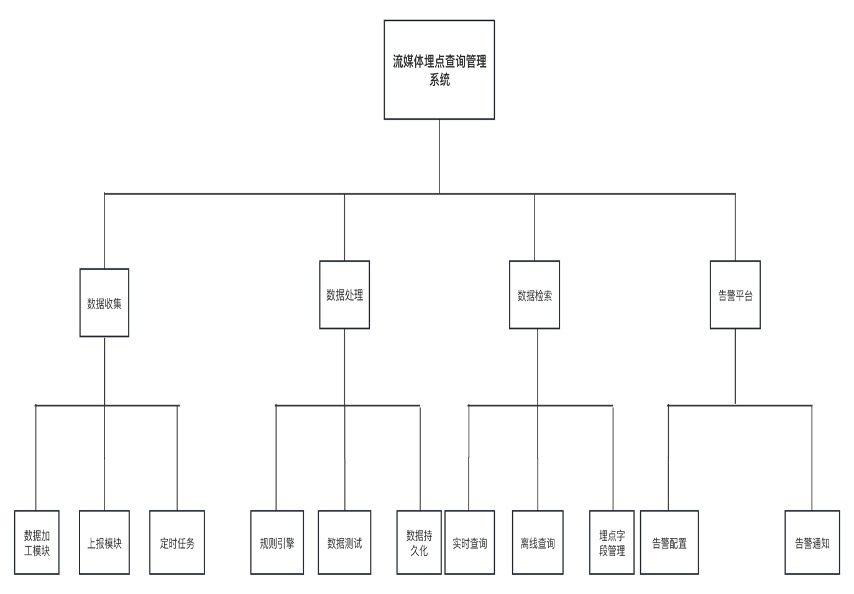
\includegraphics[width=5in]{figure/chapter4/系统功能模块划分图.jpg}
  \caption{系统功能模块划分图}\label{huafen}
\end{figure}

数据收集模块分为数据加工模块、上报模块、定时任务模块。数据加工模块是上报前的数据预处理操作,为了提高数据上报的效率和安全,可以先对数据进行加密和压缩等操作。上报模块是客户端和服务端SDK将流媒体埋点数据上报到数据中心,上报需要注意服务端带宽压力,为了避免负载超载情况下拥塞加剧,需要数据收集组件进行主动避让,降低上传间隔。定时任务是指定时拉取服务端接口的数据到数据中心。

数据处理模块分为规则引擎模块、数据测试模块、数据持久化模块。可以通过书写JQ规则对数据格式进行转化,将来源于各个数据源的数据转化为统一的格式。数据测试模块是指将数据按照规则引擎进行转化,用户可以观察转化后的结果。数据持久化模块用来将数据进行存储管理,设置好数据过期TTL和存储引擎。不同的存储引擎具有不同的使用规则,后面会详细介绍。

数据检索模块分为实时查询模块、离线查询模块、埋点字段管理模块。该
模块也是系统的核心功能,实时查询是使用二级索引去加快定位数据,首选根据
筛选条件去检索ElasticSearch,拿到符合条件的文档UUID,再根据UUID去哈希索引BMQ(存储埋点上报的完整字段)中的数据,最终拿到完整的埋点数据。ElasticSearch在其中起到过滤器的作用,降低了对BMQ的检索压力。离线查询首先将前端的筛选条件转化为HQL语句,然后提交批处理任务检索HIVE,将返回的数据写入到ElasticSearch中,并且提供一个访问ElasticSearch中这些数据的URL,这样可以做到在同一个页面上同时展示实时和离线查询的数据,对用户来说是透明的。埋点字段管理模块是采用LRU算法将最近不常用的字段过期掉,那么上游Flink就不会再将数据写入到ElasticSearch中,降低了ElasticSearch的存储压力。并且用户在进行字段筛选时,系统应提供字段分布来供用户选择。

告警平台模块分为告警配置模块、告警通知模块。该模块的作用是实时/定时监控埋点上报的字段指标,适用于基于时间序列的埋点数据流。告警配置模块可以选择窗口大小、指标字段、检测算法、阈值。当指标检测值超出阈值将以图表形式通知用户。

\subsection{系统总体架构设计}

为了更好的描述系统的整体架构,本节首先使用系统整体架构图对该系统进行描述,同时本节使用4+1视图模型来描述系统的总体架构~\cite{kruchten19954+},包括逻辑视图、进程视图、物理视图和开发视图,每个视图仅描述一个特定关注面的集合,而场景设计在第三章需求分析的用例描述中已有详细描述,此处不再赘述。

1)	系统架构图

 \begin{figure}[htb]
  \centering
  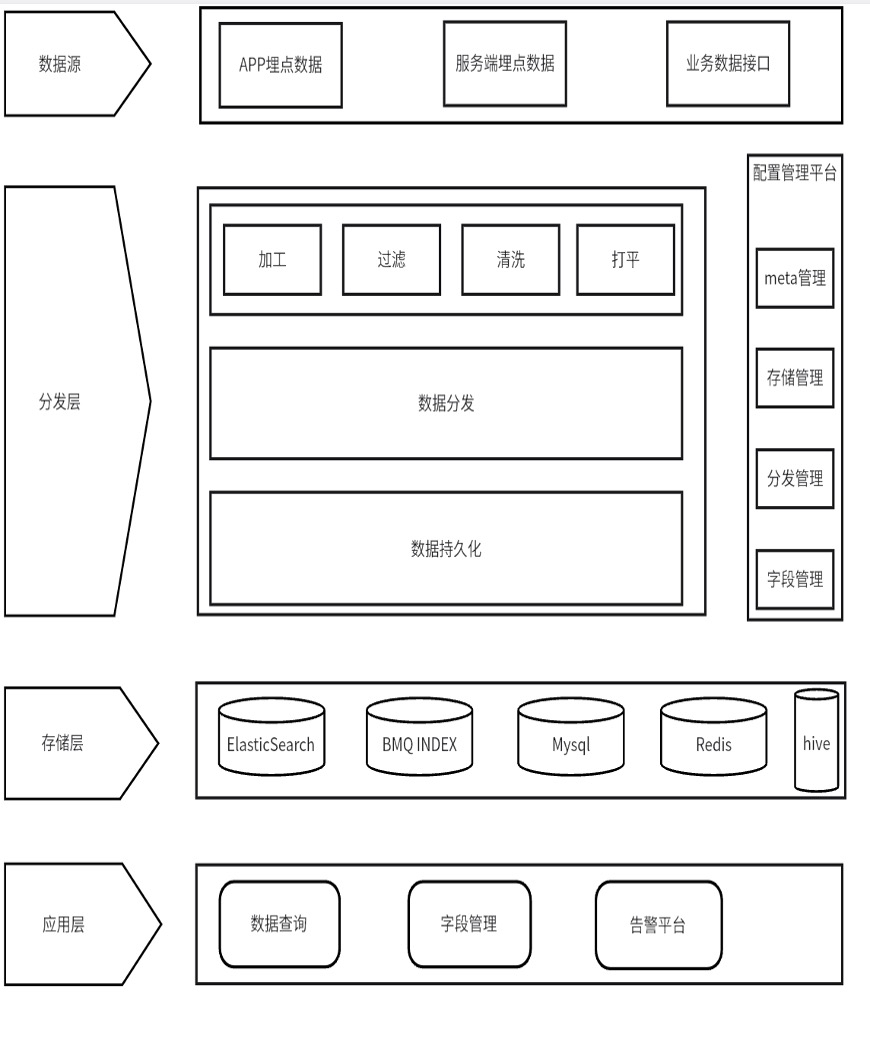
\includegraphics[width=5in]{figure/chapter4/系统架构图.jpg}
  \caption{埋点查询系统架构图}\label{xitongjiagou}
\end{figure}

如图\ref{xitongjiagou}描述了流媒体埋点查询的系统架构图,系统架构上可分为数据源接入层、分发层、存储层和应用层。所有层的配置信息统一在配置中心管理TCC。数据源的数据经过数据处理后进行数据分流,Mysql负责维护哪些字段属于索引字段、高热字段。用户可以通过API的方式,方便地将日志字段提级为索引高热字段。经由Flink任务抽取索引字段、高热字段后,分别写入ElasticSearch和BMQ Index。全量的数据也会写入HIVE中一份,用来做离线查询。ElasticSearch开启动态索引功能可以不断改变索引结构。若是需要对数据进行埋点上报监控可以使用告警平台功能,出现问题及时反馈给用户。
2)	逻辑视图
 \begin{figure}[htb]
  \centering
  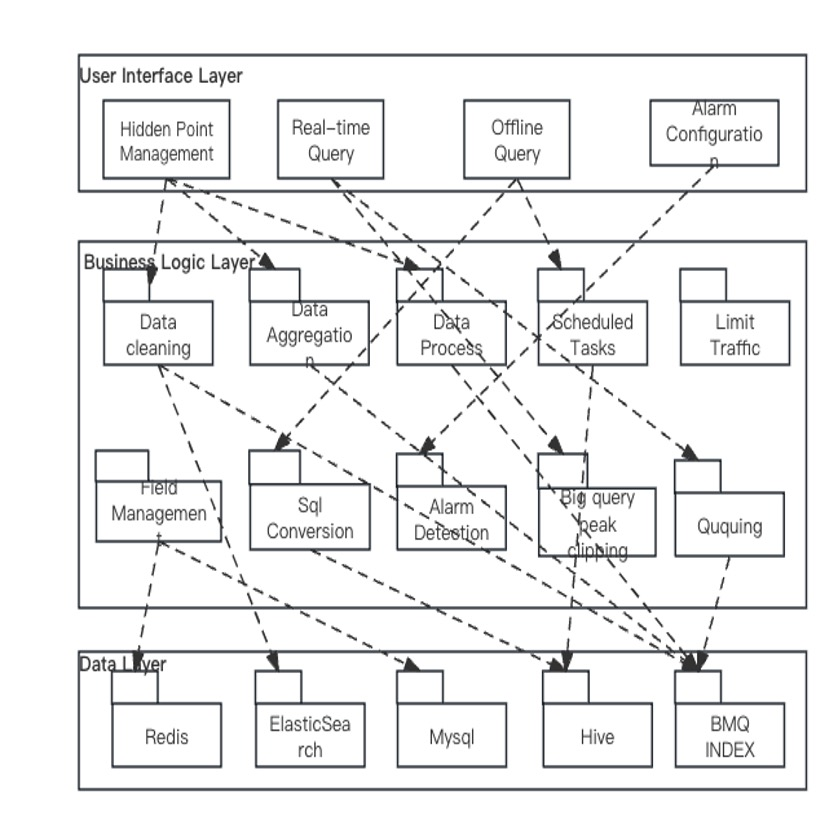
\includegraphics[width=5in]{figure/chapter4/系统逻辑视图.jpg}
  \caption{埋点查询系统逻辑视图}\label{xitongluoji}
\end{figure}

如图\ref{xitongluoji}描述了埋点查询系统的逻辑视图。该视图从功能上对系统进行拆分,其风格采用面向对象方式,重点在于将系统描述为单一且一致的对象模型,关注系统应该实现哪些功能,而并不关注其具体的技术实现。

系统在逻辑上分为三层,最上面一层为用户交互层,用来接收用户的输入和对系统结果的展示,其中包括4个部分,埋点管理、实时查询、离线查询、报警配置。埋点管理用于数据源埋点字段的增删改查,操作成功之后埋点立即生效,新增筛选埋点只能应用于筛选新数据。并且还提供了日志埋点上报数据处理规则引擎接口,用户可以通过书写JQ表达式来对数据进行处理。实时查询界面用户可以通过增加筛选字段和选择时间范围进行实时数据检索。离线查询通过书写lucene正则表达式~\cite{qian2010evaluation}来作为筛选条件,后台将其转化为SQL语句去检索HIVE。报警配置是用户手动选择报警检测窗口时间、报警检测算法、检测阈值元数据信息,提交后会生成报警检测任务来执行。

逻辑层主要分为10个部分,包括数据清洗、数据聚合、数据处理、定时任务、数据限流、字段管理、SQL转化、报警检测、大查询削峰和查询队列化。数据清洗的作用是将不符合数据规范过滤掉,数据聚合是指将一定period的数据聚合为一起共用KEY,从而达到降低写入QPS的目的。数据处理是指使用用户自定义的规则表达式JQ将原始数据格式转化为目标数据格式。定时任务的应用常见为定时扫描Mysql数据库中的离线查询任务记录,若存在未就绪则获取任务信息并执行任务。数据限流、大查询削峰、查询队列化都是对实时查询的控制,为了保障服务端的压力在可承受之内所做的优化。在接口侧,对同时执行的BMQ Index查询数进行限制,以控制BMQ集群的总负载上限。针对可能一次性返回大量日志的查询,在收到用户请求后,会对请求执行拆解,分批对BMQ Index执行查询,以降低对网络/BMQ集群的瞬时负载。在未限流时,队列不起作用,在限流的情形下,被限流的请求会被暂存入一个队列,队列按照先入先出的顺序消费请求,返回BMQ里的查询结果。字段管理是后端对埋点字段的管理,使用LRU算法过期掉超出数量限制并最久不被使用的字段,也就是上游在写入ElasticSearch时将不再写入该字段,实现这个需求需要将索引字段保存至Mysql中,写入时读出所有的索引字段来进行写入。SQL转化是指需要将前端提交的lucene正则表达式转化为SQL语句,然后提交给HIVE去执行。报警检测分为两种,分别是静态阈值算法、同比算法。静态阈值算法是指大于(>)、小于(<)、大于或等于(>=)、小于或等于(<=)阈值。同比算法的参数值是是波动值,比如配置了0.1,代表波动10$\%$。当前周期的数据和昨天同周期以及上周同周期的数据进行对比,波动超过配置的参数值就进行报警。

数据层主要分为6个部分:Redis、ElasticSearch、Mysql、Hive、BMQ INDEX。
分别负责LRU算法实现、数据的埋点索引、存储埋点字段、存储离线全量数据、存储实时全量数据。

3)	进程视图
进程视图侧重于描述系统在运行时各进程是如何交互的,关注系统运行时的行为和质量属性。如图\ref{xitongjincheng}描述了流媒体埋点查询系统的进程视图。
 \begin{figure}[htb]
  \centering
  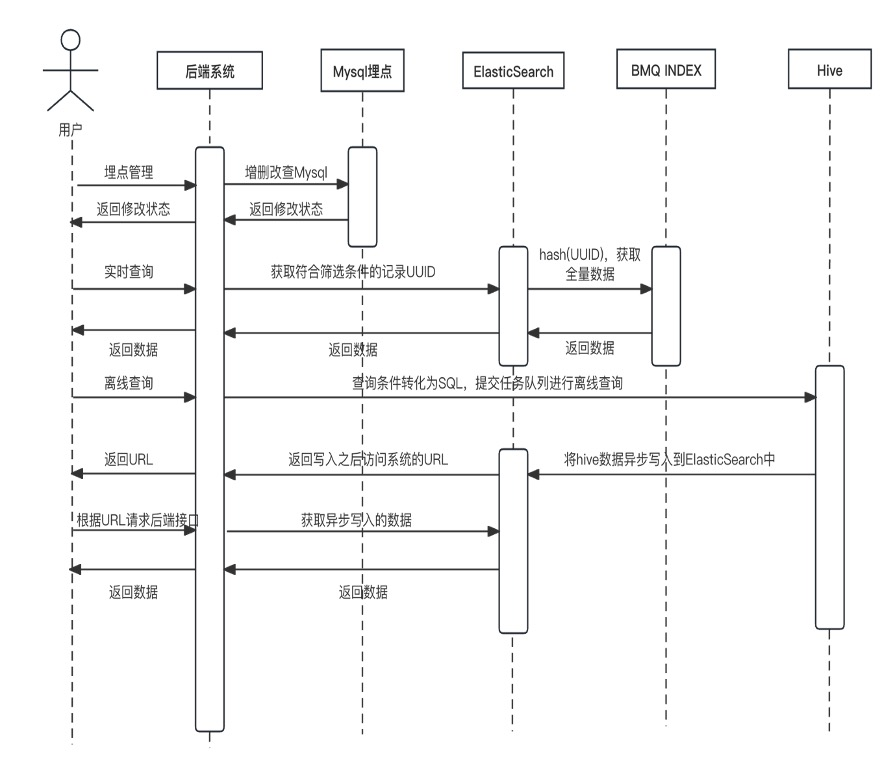
\includegraphics[width=5in]{figure/chapter4/系统进程视图.jpg}
  \caption{埋点查询系统逻辑视图}\label{xitongjincheng}
\end{figure}

在该视图中,系统由前端用户操作界面、后端服务器、APP SDK、Flink、BMQ Service、ElasticSearch、Hive和MySQL数据库组成。在流媒体埋点查询系统中,不同的服务启动单独的进程进行相互之间的访问,Web服务器通过异步调用的方式调用后台服务器提供的RESTful风格HTTP接口,避免由于后台服务忙、响应时间慢而导致前台服务器长时间的等待,缩短系统响应时间,后端服务器和Flink是通过JDBC协议与Mysql进行数据通信,都采用管理数据库连接池的策略来保证数据库连接的并发性控制。后端服务器和BMQ INDEX之间的通信是通过KiteX RPC通信,需要两者之间协商好通信的数据文件Thirft,并且后端服务器是由许多微服务相互调用构成的,它们之间的通讯都是采用KiteX服务调用。后端服务器通过RESTful风格HTTP接口与ElasticSearch进行数据的交互和获取字段的分布情况。

4)	物理视图

 \begin{figure}[htb]
  \centering
  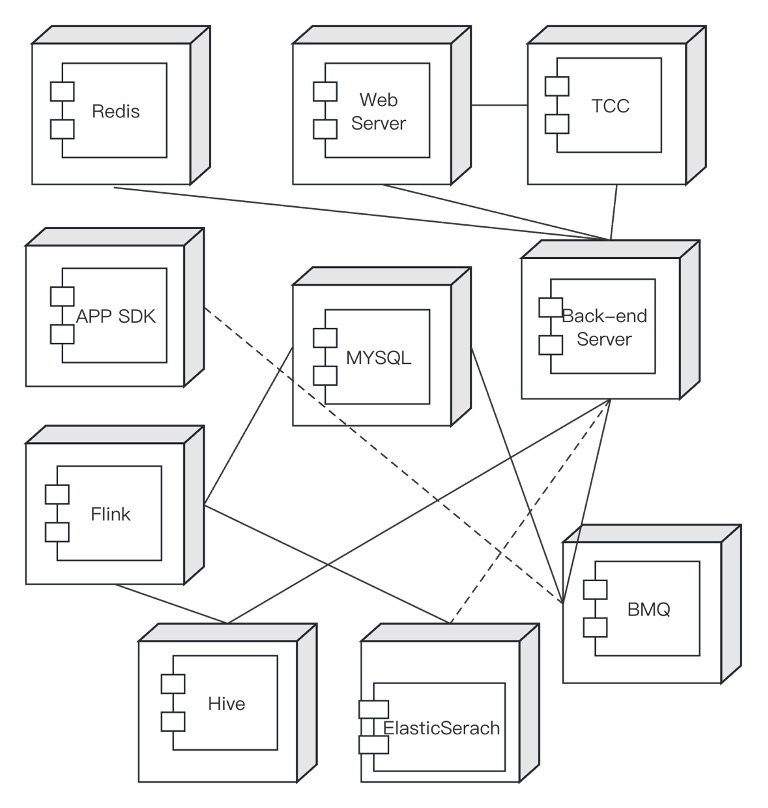
\includegraphics[width=5in]{figure/chapter4/系统物理视图.jpg}
  \caption{埋点查询系统逻辑视图}\label{xitongwuli}
\end{figure}

物理视图关注系统静态的部署视图,包括依赖的运行库和系统软件。如图描述了流媒体埋点查询系统的物理视图。

Mysql、Hive、ElasticSearch、BMQ Service、Redis、Flink分别部署在单独的云引擎集群,这样做到了资源之间的解耦,在流量的早高峰时刻可以做到水平动态扩缩容来适配流量变化。本系统前后端分离,分别部署在不同的服务器上,通过HTTP接口进行交互访问。TCC作为配置中心,也是单独部署在云引擎集群中,提供HTTP接口供其他微服务获取元数据;Flink任务是在数据平台Dorado上进行运行配置的,监听消息队列中的数据进行消费。如果Flink任务来不及消费消息队列中的数据就会产生数据堆积,这就造成下游数据的时间延迟,因此Flink需要进行更多的进程来消费消息队列中的数据,因此Flink也十分有必要进行动态扩容。BMQ设计的基本理念就是云原生,存储和计算分离,所有的持久化存储都放在云存储中,由云存储组件来保证数据的一致性和可靠性,以及相应的灾备和Geo-replication的能力,而BMQ自己的节点则可以保持本地无状态,专心处理好消息队列本身的计算逻辑,从而将计算和存储完全分离开。这样的设计也使得BMQ的节点可以很方便地容器化。ElasticSearch采用存储数据采用分片机制,可以把分片想象成数据的容器。文档存储在分片中,然后分片分配到你集群中的节点上。当集群扩容或缩小,Elasticsearch将会自动在你的节点间迁移分片,以使集群保持平衡。因此Elasticsearch也是天然支持横向扩展,可以通过增加机器来保证有足够的空间。

5)	开发视图
开发视图关注在开发过程中项目的设计决策和开发过程中项目创建的实际模块组织,在这里采用分层的结构来描述。如图\ref{xitongkaifa}描述了流媒体埋点查询系统的开发视图。
 \begin{figure}[htb]
  \centering
  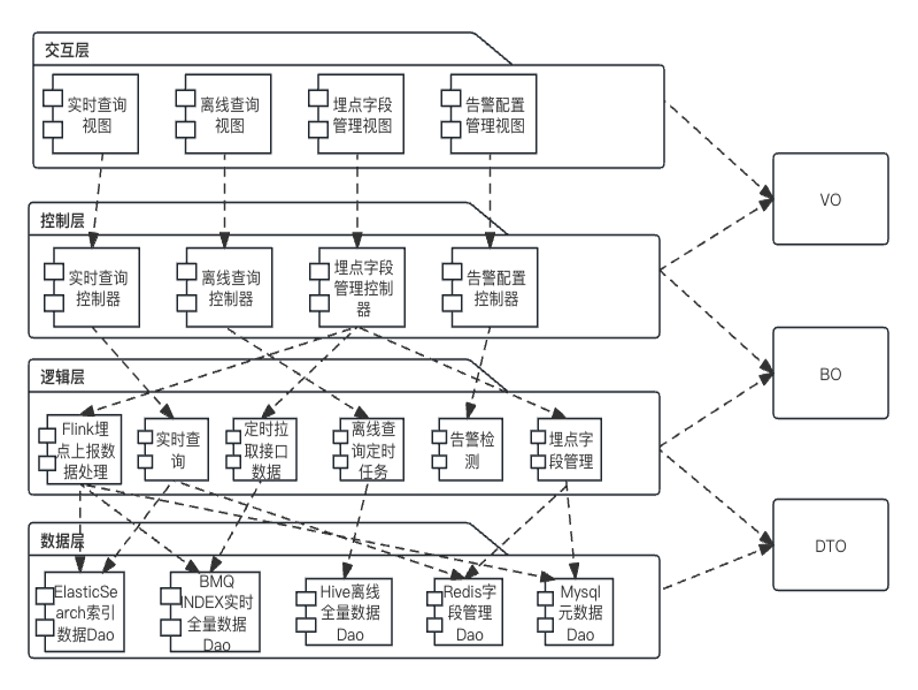
\includegraphics[width=5in]{figure/chapter4/系统开发视图.jpg}
  \caption{埋点查询系统逻辑视图}\label{xitongkaifa}
\end{figure}
在开发过程中,系统被分为4层去实现。从上到下依次是交互层、控制层、逻辑层和数据层。其中交互层包括实时查询视图、离线查询视图、埋点字段管理视图、告警配置管理视图、数据拉取视图,均采用Vue.js、Element ui和Echarts.js等技术栈来实现。

控制层包括实时查询控制器、离线查询控制器、埋点字段管理控制器、告警配置控制器、数据拉取控制器,这里基于Gin框架使用Go语言进行开发,每个控制器都向外提供一组统一的RESTful HTTP接口。

逻辑层包括Flink埋点上报数据处理、定时拉取接口数据、实时查询、离线查询定时任务、告警检测、埋点字段管理。这一层是具体功能模块的实现,用来供控制层调用。Flink埋点上报数据处理是对SDK 埋点上报的数据处理,为了保证数据处理的效率和数据不丢失,分别从数据的生产和消费角度进行优化,生产端使用Snappy压缩算法~\cite{樊书华2019一种基于流媒体压缩算法的高性能集群监控系统}对数据进行快压,并且写入MQ的时候开启Batch批写入,提高了数据高并发写入能力。消费的时候对数据进行Merge,在一段时间内的上报数据共用一个Key,减缓对下游存储的冲击。定时拉取接口数据需要申请接口拉取的HTTP Token来做为header中Authority字段值,将任务提交到Dorado进行拉取任务的具体执行。实时查询是业务的核心功能,控制层传递筛选字段选项、时间范围选项给业务层,业务层将其构造成请求ElasticSearch的DSL语句,然后再去请求BMQ INDEX。ElasticSearch是一款强大的日志搜索引擎,它基于倒排原理为存储在硬盘上的数据集制作索引,提升了从数据集内部返回所求日志的效率,同时为开发者提供了方便的日志查询抽象,提升了开发便捷度。若不选用带索引的物理引擎保存日志(例如Kafka),则每次请求,返回所求日志的复杂度是O(n),这会严重加大查询耗时。若不将日志保存于磁盘,而是直接用内存保存日志(例如Redis),虽然可能查询效率会变高,但这样会导致存储成本的急剧上升。上面提到,我们需要保存的数据集大小在PB量级,而当前商用机器的单核内存,通常只有几个GB。这就意味着这种选型可能需要准备数万台机器,仅仅为了存储这些日志。这在降本增效方面,很难说是一个好的方案。同样是成本考量问题。现阶段客户端日志的总字段数,和ES索引的字段数,大约占比在5:1左右。如果将所有字段做成索引,虽然对用户体验的提升并不会太大,但却需要准备5倍的存储空间,为了维护索引而带来的CPU消耗,这也是不经济的。在查询阶段具备KV查询能力,在我们的场景下,可以先从ES取回key,再根据key取回高热字段。由于key的数量已经在ES查询阶段被过滤,所以对BMQ Index后端的负担较为可控。离线查询的意义是因为BMQ INDEX并不是在任何情况下都是可以对外提供正常服务的,举个BMQ Read限制的例子,假如你请求BMQ Index的QPS是10,但是每个partition key对应100条数据,由于数据是存储在BMQ中,那么对于BMQ来说这里的qps就是10*100,目前建议这个值在300以下。因此你的实际请求Index的QPS不能超过300除以每个partition key下边的数据条数(即:qps*limit小于300)。并且BMQ是居于HDFS的,举个HDFS限制的例子,BMQ Index是按照索引文件的大小分割索引文件(简单理解:往文件后边追加数据,等到了阈值就创建下一个文件,同时文件名携带了和filter有关的信息)。因此索引字段越多、越大需要打开的文件就越多,此时HDFS承担的压力就越大。按照经验在写入1.7k QPS,索引包含20个字符情况下建议Filter范围在2h以内。那么离线查询的虽然比较慢,但可以保证查询的质量,查询更稳定。并且Hive数据保存时间长,可以查询更久的数据,不存在RPC调用,查询结果因此可以更大。埋点字段管理逻辑是对ElasticSearch索引字段和Mysql元数据的操作,依赖于Redis的统计信息,字段的使用情况都可以使用Redis进行记录最近使用的时间,然后后端开启定时扫描任务,如ES中索引字段数量超出了IndexedFieldsUpperBound,那么就需要过期掉超过的字段数,可以使用最小堆来进行时间堆排序,过期的字段同时更新Mysql。告警检测模块可以以接口的形式对控制层提供服务,设计模式考虑使用策略模式,因为告警检测算法是可以随机切换选择的,目前调研的检测算法主要有:简单阈值、同比阈值波动、卷积自编码器 (Convolutional Reconstruction Autoencoder Model)、孤立森林 (Isolation Forest Model)、XGBoost 预测。后面在告警检测模块将进行具体介绍。

数据层则包括ElasticSearch索引数据Dao、BMQ INDEX实时全量数据Dao、Hive离线全量数据Dao、Redis字段管理Dao和Mysql元数据Dao,该层主要是后端服务系统与存储系统的交互接口,实时查询逻辑通过查询ElasticSearch索引数据Dao获取文档UUID,根据文档UUID去检索BMQ INDEX实时全量数据Dao。

离线查询逻辑通过lucence正则转化器将lucence语句转化为SQL,提交批处理任务给Hive来获取数据。埋点管理逻辑通过Redis字段管理Dao实现LRU埋点字段过期,相应的通过Mysql元数据Dao持久化,并且Mysql元数据Dao还用来保存离线任务记录,定时轮询Mysql来执行未就绪状态的任务。

\section{流媒体埋点查询系统详细设计}
由于Go语言是灵活并不纯面向对象或面向过程的语言,因此开发人员可以根据编程习惯灵活的使用Go语言基于KiteX框架进行系统的开发。本系统与传统的面向对象系统设计不同,本系统是一个ELK系统,涉及数据上报、数据处理、数据检索、告警平台模块,模块之间很难做到统一开发语言,因为就拿数据处理来说,市面上的Flink应来做数据处理已经十分成熟,为了降低开发成本,数据处理部门使用Java开发,其他模块使用Go进行开发,面向过程和面向面向对象的风格都在代码中有所体现,在开发视图设计上仍然采用MVC~\cite{pop2014designing}的方式,将核心逻辑封装在逻辑层,我们对模块功能在逻辑层的方法上进行划分。
因此,在如下的各个模块设计上,我们通过分类方法的形式展示每一个模块设计到的用例,同时更深一步的展示每一个用例所涉及到的功能点,以此出发对本系统详细设计展开描述。

根据上述对自助压力测试系统的总体分析及模块设计,本节将依次详细介绍该系统的每个子系统的详细设计。

\subsection{埋点上报SDK详细设计}
埋点上报SDK是数据采集和上报的工具包,埋点上报SDK具有通用性, App、Android、IOS、网页都能使用该SDK来采集数据和上报。埋点上报是流媒体埋点系统的第一步,在整个数据流程处于最开始,最上游。后续的所有模块、功能或者系统,都会受到埋点上报SDK的影响。埋点上报的数据类型包括设备数据,用以唯一识别一个设备,尤其当用户未登录App时,通过设备来区分用户;行为数据,也就是埋点数据,应用在用户交互的操作流中,找到关键事件进行埋点,当用户触发关键事件,应用就会将事件埋点交给SDK,SDK采集到埋点,上报给后台。当用户登陆账号或账号切换时或App收集到用户的其他信息时,可以将用户信息交给SDK,SDK上报到后台做统一处理。

上报的整体流程为APP通过SDK将客户端产生的日志上报到SDK收集服务对应的URL,请求被打到对应的机房的入口Nginx网关,网关将请求转发到SDK服务所在的负载均衡集群~\cite{ghomi2017load},负载均衡集群将接收到的请求转发给SDK收集服务,并对收集的日志补充必要字段信息,并将上报流入下游的BMQ消息队列。
 \begin{figure}[htb]
  \centering
  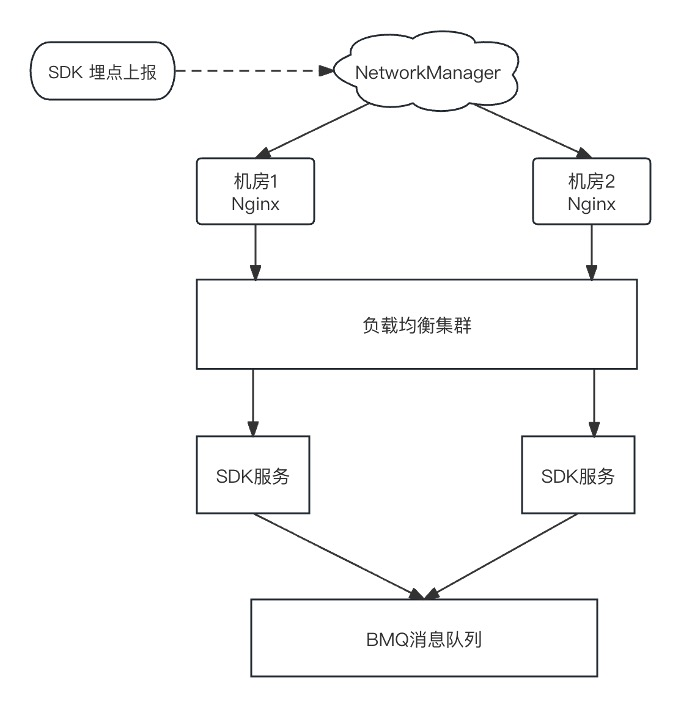
\includegraphics[width=5in]{figure/chapter4/埋点上报流程图.jpg}
  \caption{埋点上报流程图}\label{maidanliucheng}
\end{figure}

然后,介绍一下埋点上报模型,首先介绍一些基本概念,有两点需要说明,第一,后台Launch,也就是后台运行时,有事件上报,会产生一个后台Launch,用来标示一个后台Session的开始。第二,Terminate时机,IOS是在用户切后台后,立刻算作Session结束,会产生一个Terminate事件;而Android是当用户在后台停留30s后,才产生Terminate。

埋点上报模型如下图\ref{maidanshiji}所示,上报间隔为每60s上报一次。Android延迟30s才产生Terminate的原因应该是某个程序员从技术角度做的设计。Android一直有“后台可运行”的概念,用户暂时离开App,App还可以在后台运行,那么在短时间内回到App,还是同一个进程。同一个进程,对程序员来说,App没重启就当作同一个Session。至于为什么30s,应该是想总不能无限长吧,就设置成30s。
 \begin{figure}[htb]
  \centering
  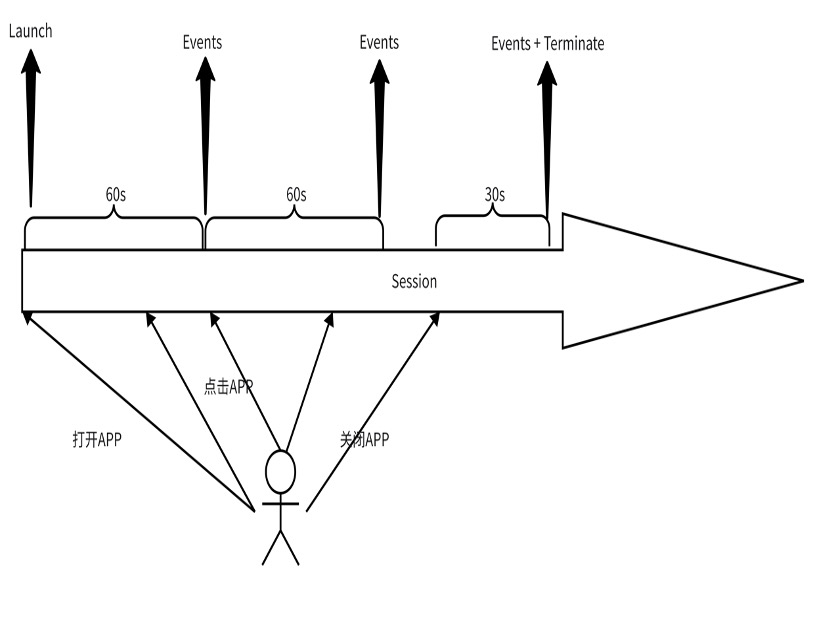
\includegraphics[width=5in]{figure/chapter4/埋点上报时机图.jpg}
  \caption{埋点上报时机图}\label{maidanshiji}
\end{figure}

下面介绍Session、Launch、Terminate事件发生时机:
1)	Session:用户在App上的一次会话,也就是从打开App,连续使用到切后台,这一段连续的前台交互,叫做一个session。不管这个交互有多长,交互有多少,只要在前台,就是一个session,不会结束。所有埋点上报的事件,都有一个SessionId字段,也就是说事件是挂在session下的。关闭屏幕,对app来说就是“切后台”。iOS会立刻结束session,Android等30s结束session。那么对于Android,有“后台启动”的情况,后台运行时也会上报的事件,这时,也需要一个Session,所以,有“后台”Session的概念。Session是一个会话概念,每个上报事件都有sessionId字段,但session本身没有直接对应的上报事件。标示一个Session的开始和结束,使用的是Launch和Terminate两个事件。

2)	Launch:当用户启动App(切前台)的时候,SDK内部会产生一个Launch事件。

3)	Terminate:当用户停止使用App,将App切换到后台后,SDK会产生一个Terminate事件。

下面介绍一下上报的埋点数据,埋点数据格式是以JSON格式定义,它的格式是这样的:

  \begin{figure}[htb]
  \centering
  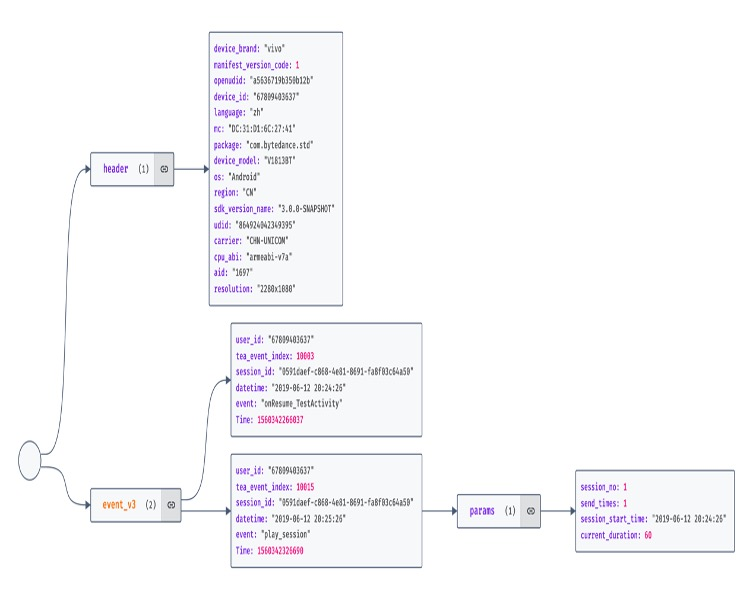
\includegraphics[width=5in]{figure/chapter4/埋点上报数据结构.jpg}
  \caption{埋点上报数据结构}\label{maidanshujujiegou}
\end{figure}
1)	Time: 调用SDK方法onEvent时的时间。SDK内部赋值的,外部不可修改。如果想修改time,不如自己在自定义参数中定一个新的字段my\_time。

2)	Session\_id: 是调用时的sessionId。SDK内部赋值的,外部不可修改。

3)	Param: json格式可以自定义一些字段。不过,有一些约定,仅接受int、string、float。

4)	Header:SDK会上报的通用信息,每个event里都有header。信息比较多。是SDK内部自动收集并上报的通用信息,所有事件都可以共用这些信息。业务新增埋点时,各自不需要再重复采集这些信息了,后台可以直接从Header里读这些信息。

5)	Event:比较重要的字段,是唯一区别一个事件的字段,需要在app内唯一。说到唯一不能用launch、terminate这些内部关键字,然后server要加一些前缀,这是一些规范。
以上详细介绍了数据上报的Event、以及不同操作系统Session中上报流程、还有对于埋点中台的限流操作,类图如下图\ref{maidanshangbaoclass}所示:
   \begin{figure}[htb]
  \centering
  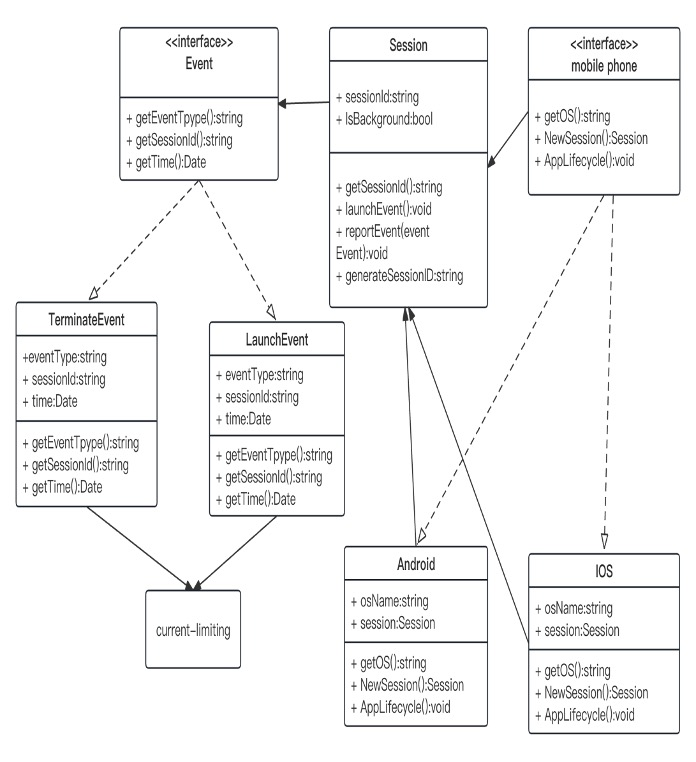
\includegraphics[width=5in]{figure/chapter4/数据埋点上报类图.jpg}
  \caption{数据埋点上报类图}\label{maidanshangbaoclass}
\end{figure}

\subsection{数据拉取pullData工具详细设计}

数据拉取工具pullData是拉取式数据接入平台,支持HTTP接口的定时请求,并将数据落入Hive、Redis或BMQ中。pullData核心模块为数据拉取,数据处理,数据导出三个模块。数据拉取模块构造符合接口要求的请求并拉取数据,数据处理模块从拉取的数据中提取所需要的字段,数据导出模块检查处理后的数据格式,并导出到Kafka中。提供定时功能,实现任务的定时执行。

数据拉取模块主要负责从外部服务拉取数据,首先读取MySQL配置参数或前端发送的测试参数,针对该配置中的参数进行解析,如:${date}/${cache}等。解析后进行参数替换,如有限流,则需构建多个请求,同时针对不同平台采用不用鉴权方式。最终发送该请求获取数据。
    \begin{figure}[htb]
  \centering
  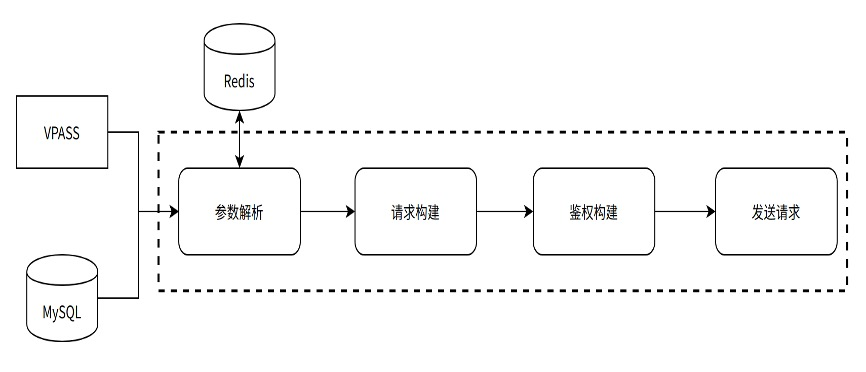
\includegraphics[width=5in]{figure/chapter4/数据拉取流程图.jpg}
  \caption{数据拉取流程图}\label{shujulaquliucheng}
\end{figure}

数据处理模块将请求得到的数据进行处理,目前只有JQ一种处理工具。JQ是一个轻量级且灵活的命令行 JSON 处理器,具有零运行时依赖性,可以轻松地切片、过滤、映射和转换为结构化数据。数据导出模块根据我们的配置,将处理后的数据写入BMQ或Redis,如图\ref{shujulaquliucheng}所示:

     \begin{figure}[htb]
  \centering
  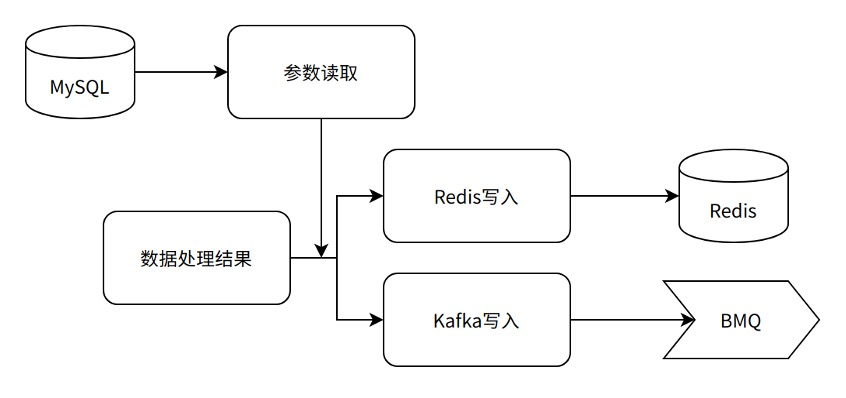
\includegraphics[width=5in]{figure/chapter4/数据持久化流程图.jpg}
  \caption{数据持久化流程图}\label{shujulaquliucheng}
\end{figure}

以上对数据拉取流程进行了详细的介绍,下面将从实现的角度对该模块进行类图展示,如下图4.13所示:Handler为Http接口处理类,前端可以进行create、query、update、open、close、delete任务,并且可以测试拉取Http接口数据,并对其进行数据处理,以供用户进行目标数据的观察。Scheduler类主要为任务提供调度功能,Flink任务可以依赖第三方Dorado平台进行管控,也可以使用Java自身的定时器进行任务调度,这些都可以供用户选择。Exporter为数据导出工具,Scheduler类依赖该类对数据进行持久化。

      \begin{figure}[htb]
  \centering
  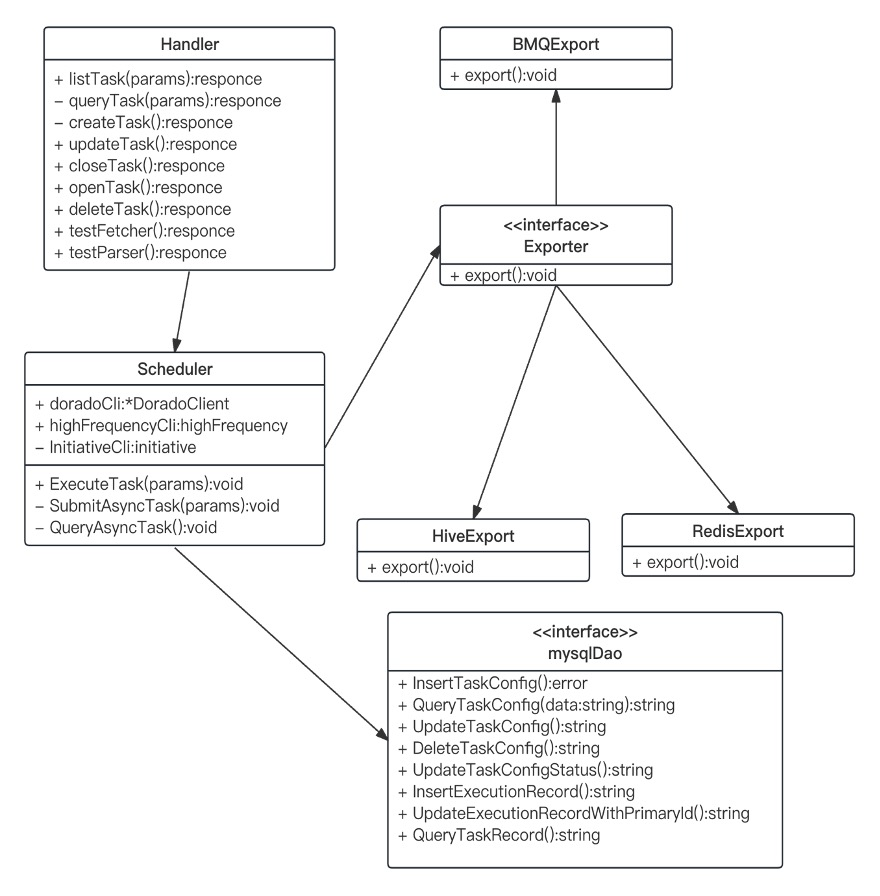
\includegraphics[width=5in]{figure/chapter4/数据拉取类图.jpg}
  \caption{数据拉取类图}\label{shujulaquliucheng}
\end{figure}

\subsection{数据处理详细设计}
上面详细描述了数据收集的主动上报和服务端拉取两种具体实现方案,那么有了数据就需要对数据进行处理来满足高质量数据的需求。数据处理面对的主要挑战是超大的数据吞吐量,这就要求早高峰系统数据处理动态扩展性,并尽可能提高数据处理能力,降低写入延迟。这个延迟是指数据产生的时间和数据经过处理后持久化的时间之间的差,如果延迟很大的话,那么就会影响对BMQ INDEX中数据的检索增大范围,降低了检索的性能。

数据经过详细数据处理方案后,应保证数据不丢失、不重复。充分利用并发处理的特性,对数据进行压缩、聚合~\cite{jesus2014survey}来优化数据处理的效能,应确保数据高效落盘,缩小写入时间和事件时间的差距。具体实现上来说数据处理并没有与系统其他模块一样采用Go语言开发,而是充分利用Flink原生语言Java开发,并且将Flink任务提交至Dorado数据平台,可以做到资源的动态调度,也就说可以灵活应对流量早高峰的大数据处理。

下面将首先进行整体数据处理的设计,然后再从数据加工管理、数据持久化角度对数据处理进行详细方案设计。

数据处理与数据查询和管理相辅相成,Trace系统两大功能分别是查询和字段管理。查询涉及ElasticSearch、BMQ INDEX和HIVE三大数据源,这就要求上游数据做好数据分流,而数据能够分流同样依赖MYSQL中的埋点字段信息,Flink任务能够监听MYSQL中索引字段的变化,从而实时的对数据进行分割,使得索引数据流向ElasticSearch。前端也提供了索引字段的增删改查,这同样是操作的MYSQL埋点表。那么整体数据处理如下图\ref{zhengtishujuchuli}所示

\begin{figure}[htb]
  \centering
  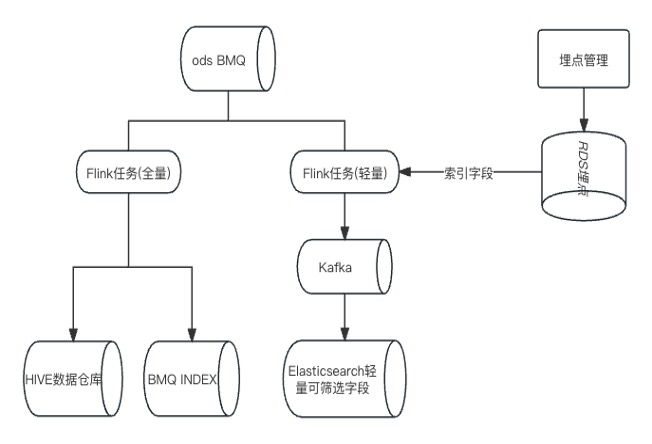
\includegraphics[width=5in]{figure/chapter4/整体数据处理流程图.jpg}
  \caption{整体数据处理流程图}\label{zhengtishujuchuli}
\end{figure}

数据加工是提高数据处理能力的重要手段,Trace系统对数据进行了Snappy压缩、以及将短时间内的数据聚合共用Key。Snappy压缩具有压的快、解的快的特性,能够保障数据处理速度的同时也保障了数据查询的速度。目前日志晚高峰写入异常比较严重,BMQ INDEX无法扛住写入的QPS。为了应对日益增长的流量,需要对BMQ INDEX数据导入进行优化。记录结构一般为<PK:CK,Value>,PK为app\_id:device\_id, CK为timestamp,优化后Value代表某个用户某个period内的日志聚合。CK为period开始时间,Value为[event\_1\_len,event\_1\_bytes]、[event\_2\_len,event\_2\_bytes]…[event\_n\_len,event\_n\_bytes]。使用Flink开发,大部分字段清洗逻辑后移到查询阶段,Flink作业中直接聚合原始日志,未来也可以根据TCC配置加入灵活的过滤逻辑。原则是尽量减少Flink作业重启次数,避免数据异常。

维护两个Map:Map[PK, Seq[log]], Map[PK, start\_process\_time]。当某个PK 的 current\_time - start\_process\_time > 合并区间period + 随机值,触发对Seq[log]中的日志按照event time分段。假设Seq[log] 中有7条日志,根据event time排序后,按照period长度分段,注意需要确保每个分段中最后一个点存在日志,如下图所示。日志聚合到对应分段后,分段的起始位置作为该段合并后的CK,Value经过Snappy压缩,流向下游Sink中。因此区间查询[start, end) 结果返回和之前会有一些差异:多次分页请求数据,页内数据确保有序,页间数据无法确保有序。如有需求,需要前端对所有已获得的数据再进行一次排序。返回数据>=limit, 第一页会可能会出现 [start-5min, start)的数据,如有需求,前端判断可删除。精确查询单条数据[start, start+1),可能单次请求会有多条数据,需要二次筛选;也可能结果不在首页中,需要按照分页多次请求,原理图如图\ref{shujujuhegeshi}所示

       \begin{figure}[htb]
  \centering
  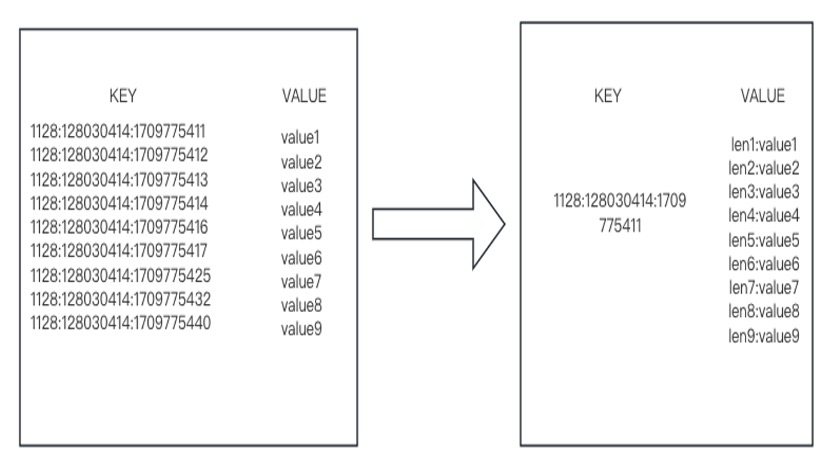
\includegraphics[width=5in]{figure/chapter4/数据聚合格式转化.jpg}
  \caption{数据聚合格式转化}\label{shujujuhegeshi}
\end{figure}

数据加工采用Flink进行开发,下面将从Flink算子角度对数据处理流程进行梳理。考虑到系统数据类型复杂,不同的数据会采用不同数据处理流程,下面就以一种通用流程进行过程展示:

        \begin{figure}[htb]
  \centering
  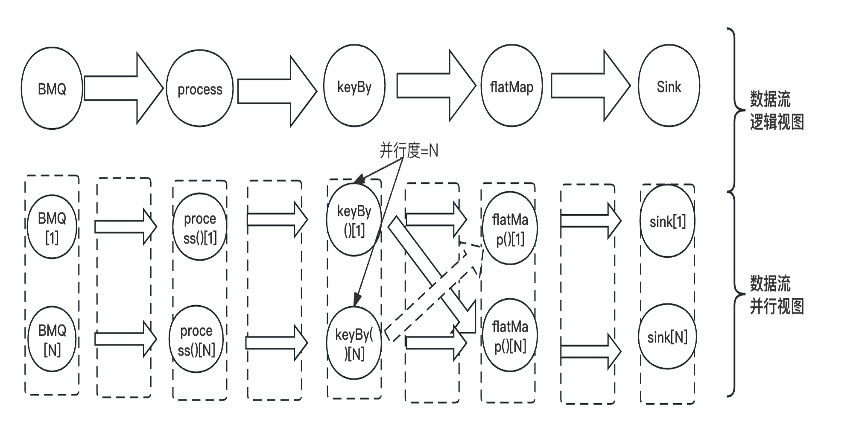
\includegraphics[width=5in]{figure/chapter4/Flink数据流图.jpg}
  \caption{Flink数据流图}\label{flinkshujuliutu}
\end{figure}

正如图\ref{flinkshujuliutu}所示,数据首先经过process算子对数据进行处理和过滤筛选,然后使用keyBy算子按照Key进行分区,再经过flatMap对数据进行Merge后分别落盘。不同的数据类型有不同的算子具体实现,以接口的形式对外暴露。
并且数据处理对数据进行管理,充分保证了Exactly Once语义~\cite{patel2014towards}。通过开启Checkpoint机制,将流处理状态和运算位置定期保存到Checkpoint,发生失败后可以从Checkpoint恢复继续执行,即输出先写入WAL,然后再提交到下游系统。发生失败可以从WAL恢复丢失的数据。输出操作使用两阶段提交协议~\cite{许海洋2011分布式事务两阶段提交协议的实现方法研究},要么完全成功要么完全失败,保证没有部分提交。使用可以重复调用的Sink,同一记录的多次输出只会执行一次。这也是使用Java、Scala语言进行开发的重要原因,Flink生态对此有着充分的支持,降低了保障数据安全的开发成本。Flink自带的checkpoint功能可以保证日志消费的不重不漏,仅通过一行Java代码配置开启checkpoint。在生产环境中设置每5分钟对程序状态执行1次checkpoint,每次执行的CPU耗时仅为500ms左右。可以认为,在对日志清洗效率影响可以忽略的前提下,实现了日志的一致性。Flink on Yarn在横向扩展效率上,显著强于Go on Cloud。在明确单核消费能力的前提下,若上报日志数出现抖动,在Dorado平台上可以便捷地增加TaskManager数,以消除端到端堆积。同样的功能在cloud平台上的流程链路则要更长些。

数据需要持久化到HIVE、BMQ INDEX和ElasticSearch中,这三种持久化的方式存在差异,BMQ INDEX其实是一种基于HDFS的KV型队列,与其他两者存在巨大的差异。对于ES业务方将消息推入消息队列中并建立Flink任务来消费写入ES,这样能保证消息写入的可靠性,在集群故障时避免了数据丢失,也能通过Flink任务来实现限速限流等功能。三者写入流程存在比较大的差异,对比如下图\ref{butongshujuyuan}所示:

\begin{figure}[htb]
  \centering
  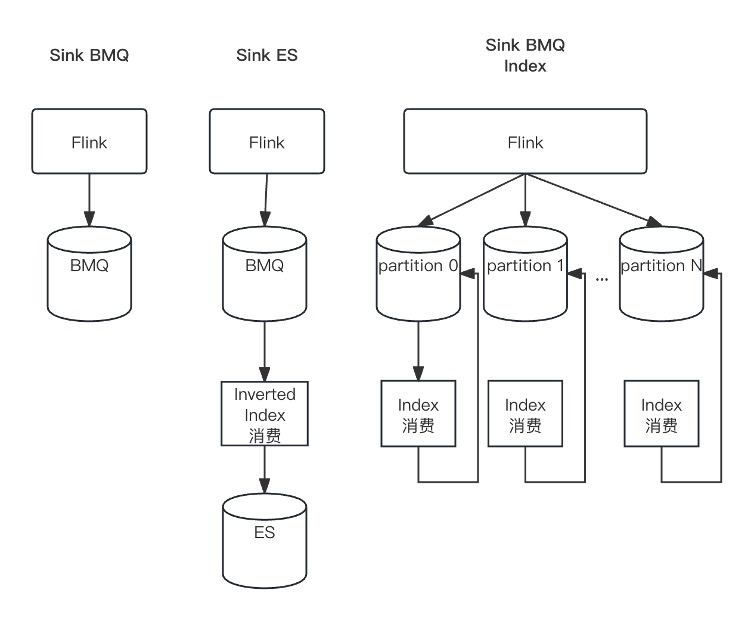
\includegraphics[width=5in]{figure/chapter4/不同数据源落盘流程图.jpg}
  \caption{不同数据源落盘流程图}\label{butongshujuyuan}
\end{figure}

其中,日志在写入BMQ Index时,必须选用指定的SDK类org.apache.kafka\linebreak.clients.producer.internals.DefaultPartitioner来确定写入哪个分区。这是因为DefaultPartitioner对于日志log的key满足DefaultPartitioner.getPartition(key,numPart\linebreak ition)=somePartition,假设key=getKey(log),DefaultPartitioner.getPartition(key1,n\linebreak umPartition)=DefaultPartitioner.getPartition(key2,numPartition),若对于日志log1、log2满足以上假设,但log1、log2写入了不同的分区,则必有一条日志无法被读取到。也就是说,每条log必须根据key写入指定的那一个分区。这就和普通的Sink BMQ场景不一样了,写入无索引的BMQ时,每个Flink slot可以任选一个BMQ分区写入,对集群的瞬时请求量是O(N)。但写入BMQ Index时,每个Flink slot里的日志,在不考虑数据倾斜的情况下,可能写入任何一个BMQ Index分区,这就导致集群瞬时请求量上涨到O(N*M),从而带来集群网络和CPU资源的负担。(假设N=BMQ分区数,M=Flink slot数)。下图\ref{bmqindexyouhua}描述了导致性能下降的情况:

 \begin{figure}[htb]
  \centering
  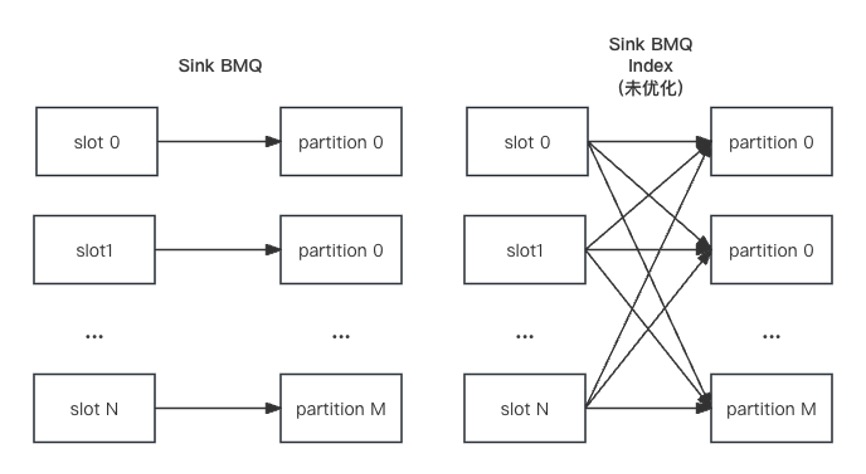
\includegraphics[width=5in]{figure/chapter4/BMQ INDEX优化前后写入对比.jpg}
  \caption{BMQ INDEX优化前后写入对比}\label{bmqindexyouhua}
\end{figure}

所以对Flink日志清洗模块作了相应的改造:将DefaultPartitioner的调用逻辑上推,然后用平凡的partitioner(不作任何处理)代替执行写入BMQ Index若对于日志log1、log2满足。写入前通过调整linger.ms、batch.size\cite{wu2019performance}、max.request.size等BMQ参数,攒批写入,降低瞬时写入请求量。实践证明,在单条日志大小约为2KB的前提下,将单次请求大小控制在100KB左右(积累50~60条日志后调用写入请求),可以达成Flink内存、BMQ集群负载之间的较好的平衡。下图\ref{bmqindexyouhuahou}描述了优化后的写入侧结构:

  \begin{figure}[htb]
  \centering
  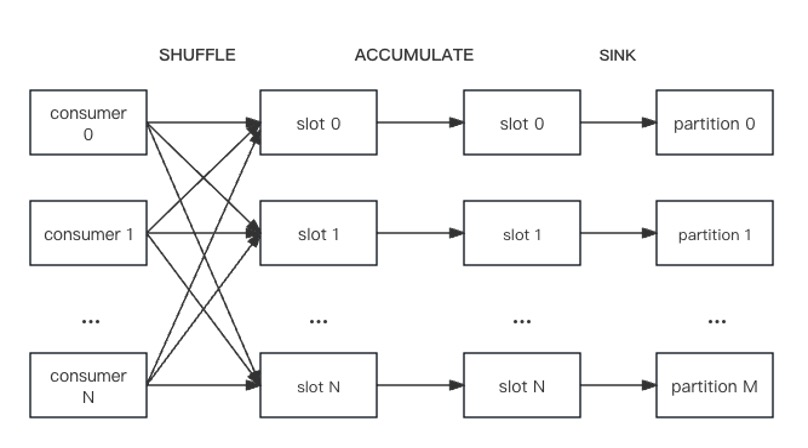
\includegraphics[width=5in]{figure/chapter4/BMQ INDEX优化后写入.jpg}
  \caption{BMQ INDEX优化后写入}\label{bmqindexyouhuahou}
\end{figure}

以上对数据处理流程进行了详细的介绍,下面将从实现的角度对该模块进行类图展示,如下图\ref{shujuchulileitu}所示:
   \begin{figure}[htb]
  \centering
  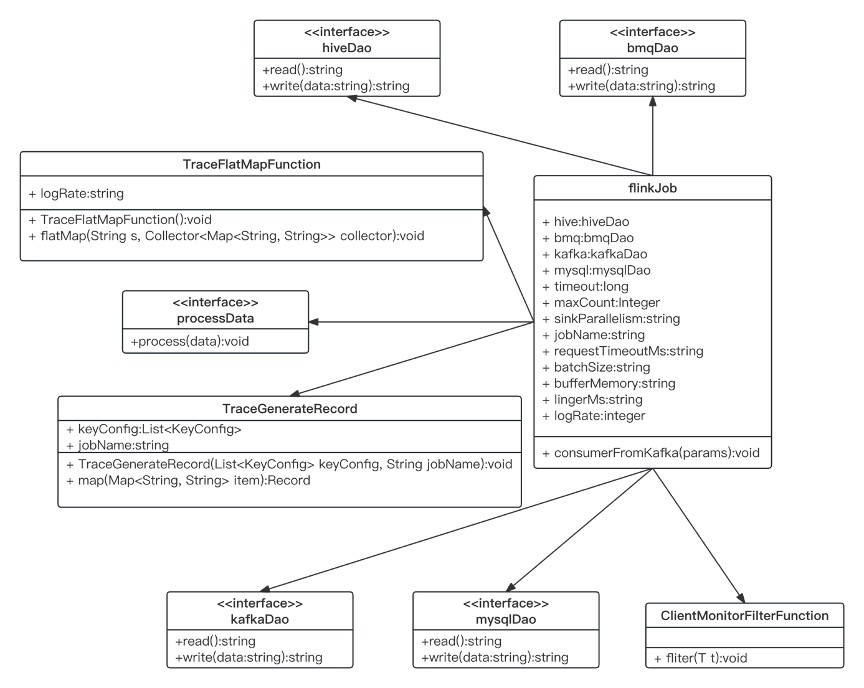
\includegraphics[width=5in]{figure/chapter4/数据处理模块类图.jpg}
  \caption{数据处理模块类图}\label{shujuchulileitu}
\end{figure}

\subsection{数据查询详细设计}
经过上面的数据上报、数据处理等基础环节后,数据被持久化。那么接下来就是对数据进行利用,考虑到业务的需要,目前系统对数据的利用仅支持数据点查、告警平台两大功能。对于数据的查询最基本的要求就是要求系统能够正确的返回数据,然后再就是非功能性功能,例如:实时性和数据可靠性。另外,考虑到系统的可扩展性,未来会接入更多的数据源,系统的架构应灵活设计,以接口的形式对外暴露。

系统采用Go语言进行开发,Go语言既可以作为面向对象和面向过程的万能语言。那么下面对系统进行设计将考虑具体的开发需求来展示详细流程。对于查询依次介绍实时查询、离线查询。系统基于BMQ INDEX设计的实时查询,存在一定的功能缺陷,因此也设计了监控大盘对查询成功率进行统计,并且设计了优化方案来提高查询成功率。离线查询能够保证100$\%$的成功和超长的TTL数据过期时间,能够检索很久以前的数据,唯一缺点就是不能保障实时性。

对于查询将首先从整体流程展开详细设计,然后逐步细化查询的具体流程。整体数据查询流程如下图所示:

 \begin{figure}[htb]
  \centering
  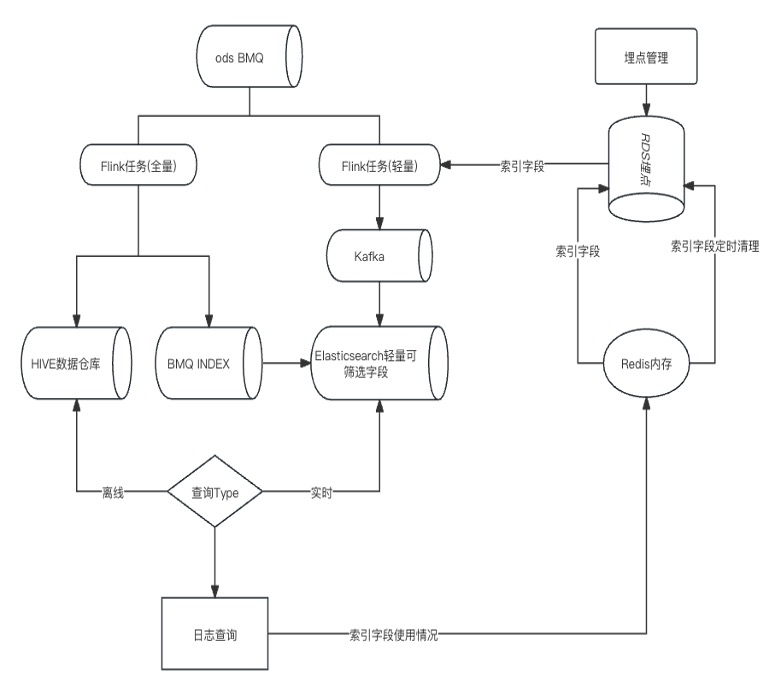
\includegraphics[width=5in]{figure/chapter4/查询详细设计.jpg}
  \caption{查询详细设计}\label{chaxunxiangxi}
\end{figure}

图\ref{chaxunxiangxi}详细描述了数据查询的详细流程。首先从用户的角度出发,可以选择离线和实时两种查询,用户选择好筛选的字段和时间范围,后台会将字段最近一次的使用时间使用Redis进行记录,会启动一个定时任务采用LRU算法进行字段数量的控制,并且更新Mysql中的索引字段信息。实时查询和离线查询的流程在需求分析时也进行了详细介绍,下面就进一步进行系统实现的详细设计方案。
\clearpage
对于实时查询来说,其设计更偏向于流程化,因此以流程图的形式进行详细描述,如下图 \ref{shishichaxunxiangxi}所示:

  \begin{figure}[htb]
  \centering
  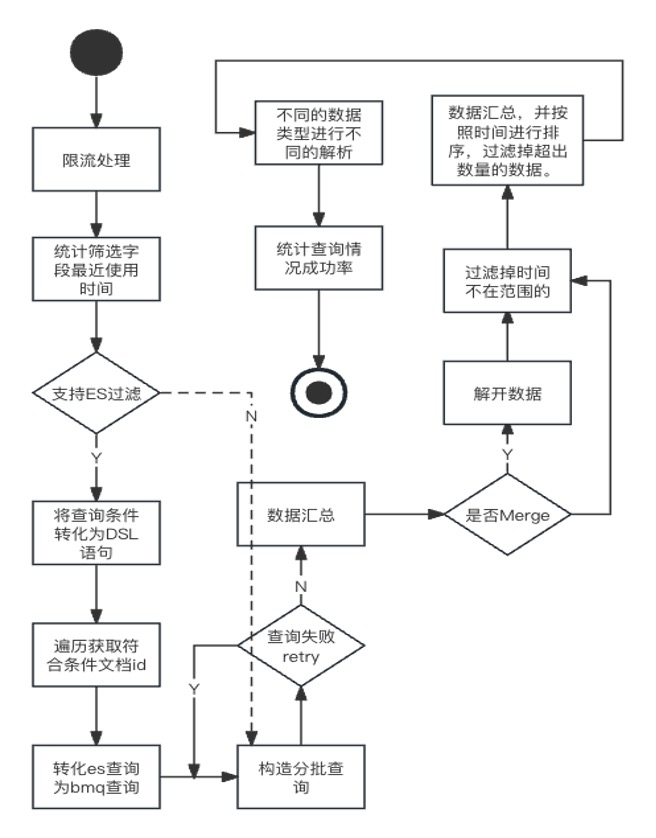
\includegraphics[width=5in]{figure/chapter4/实时查询详细设计.jpg}
  \caption{实时查询详细设计}\label{shishichaxunxiangxi}
\end{figure}

根据上图进行具体的分析,首先系统进行请求限流处理,超出QPS承受能力就会拒绝服务,前端提交的筛选字段也就是最近使用的字段,那么就会在Redis中更新它的使用时间。不同的数据类型在TCC中配置了是否支持ES过滤,也就是说不支持就直接检索BMQ INDEX,这是因为BMQ INDEX目前也支持了一定的范围范围查询的能力。如果支持ES过滤,则将查询条件转化为DSL语句进行查询。提取ES返回结果中的id和time来构造BMQ查询条件,并且应限制请求BMQ INDEX的查询QPS,这里采用分批查询。在查询失败时,会采用退避算法进行重试,将每次查询的数据进行汇总。在BMQ中存储的数据是被聚合的,在上文也提及过。因此,查出来的数据需要“解开”,也就是一个Key对应好几条数据的情况需要变为单个Key对应单个记录。由于数据持久化时间和数据产生时间是存在差异的,因此需要进行进一步过滤掉不在查询范围内的数据,并按照时间进行排序,返回指定数量的记录,因为前端设计是分页查询,一般给后端提交时都会有数量字段。在点击下一页时,会将上一页数据最后一个的时间作为查询条件时间的开始再次发起相同的查询流程。

离线查询和实时查询为了方便用户的检索,都应在同一个界面进行设计,由于离线查询结果返回时间并不是可控的,就必须设计一个定时任务进行监控,将记录异步写入到ES里面,这里为了提高ES集群的可靠性和高可用性,将数据首先写入消息队列中,然后使用Beats脚本程序将数据进行导入,并异步通知用户用户URL,这个URL其实就是打开前端的链接,并且请求了后端异步导入ES数据的接口。
   \begin{figure}[htb]
  \centering
  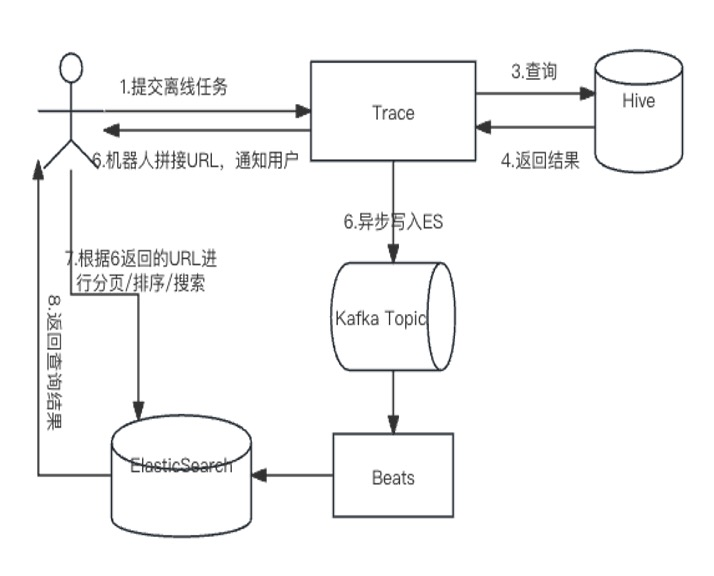
\includegraphics[width=5in]{figure/chapter4/离线查询整体详细设计.jpg}
  \caption{离线查询整体详细设计}\label{lixianzhengti}
\end{figure}

对于离线查询来说,其设计也偏向于流程化,因此流程图的形式进行详细描述,离线查询的目标:查询的方法尽量保持和目前Trace的前端一致,不改变用户习惯。单次查询的时间跨度最大支持1天,将单次离线查询时间控制在30分钟内,能够访问数据条数至多为3万条。离线查询完成后,结果以办公软件消息的形式推送给特定用户,用户点击消息中包含的URL查看查询结果,展示结果的方式和目前Trace尽可能一致,能够支持分页/排序,展示特定字段。能够在离线查询获得的结果集上,进行进一步的搜索,排序等操作,方便排查问题。首先将用户前端填写的Lucene语句和筛选项转换成Lucene语法,判断Lucene语句是否合法,如果不合法返回错误信息。将Lucene语句转换为SQL语句,异步提交TQS任务,将TQS返回的task\_id和query等参数存入RDS。返回提交成功的信息。前端收到离线如下图 
    \begin{figure}[htb]
  \centering
  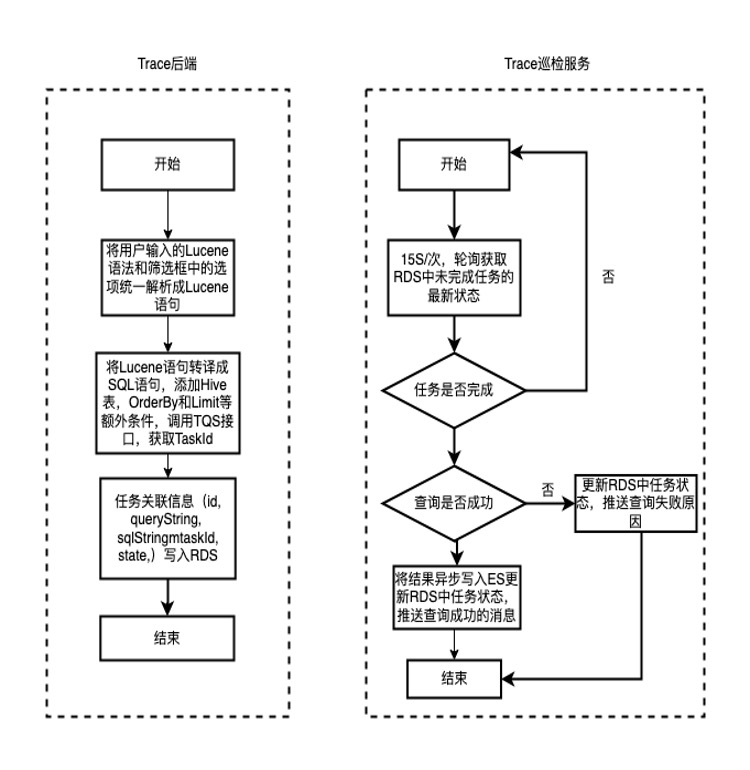
\includegraphics[width=5in]{figure/chapter4/离线查询详细过程.jpg}
  \caption{离线查询详细过程}\label{lixianxiangxi}
\end{figure}

然后,定时任务进行状态更新,流程如下图所示:巡检服务15秒每次,查询RDS中尚未被标记结束的任务。根据task\_id获取任务最新状态,若查询失败则推送给用户失败原因。若查询成功,则获取查询结果,并将查询结果中为NULL字段去除,然后写入Kafka。ES索引以uuid为doc\_id,进行去重,避免数据重复写入,写入完成后飞书消息推送查询结果给用户。

    \begin{figure}[htb]
  \centering
  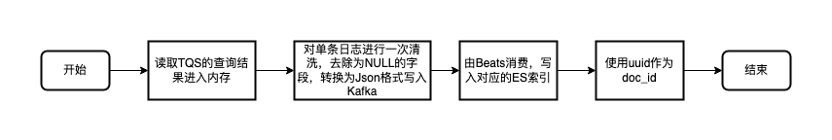
\includegraphics[width=5in]{figure/chapter4/离线查询任务状态更新流程.jpg}
  \caption{离线查询任务状态更新流程}\label{lixianxiangxi}
\end{figure}

除了定时轮询Mysql中的任务记录,还需要定时对Redis中的索引字段进行清理,其清理原理是将Redis中最近使用的字段拿出来,在内存中对时间进行小顶堆排序,选取出前50条字段来更新Mysql中的记录,从而影响上游的数据处理持久化到ElasticSearch。
以上对数据实时查询和离线查询流程进行了详细的介绍,下面将从实现的角度对该模块进行类图展示,如下图\ref{chaxunclass}所示:

    \begin{figure}[htb]
  \centering
  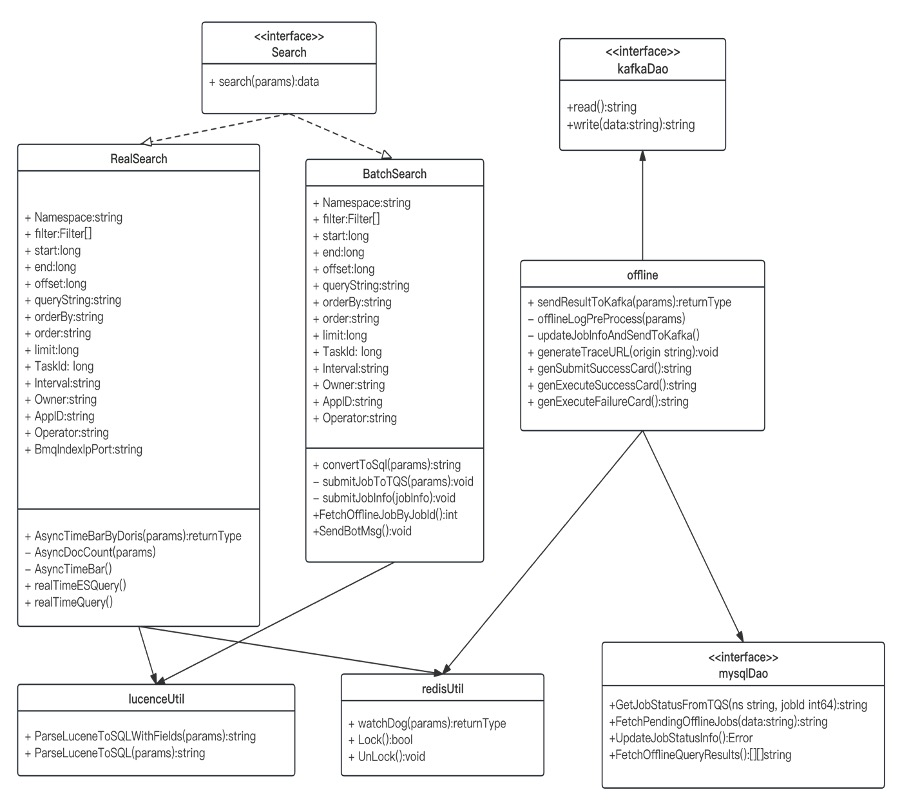
\includegraphics[width=5in]{figure/chapter4/数据查询模块类图.jpg}
  \caption{数据查询模块类图}\label{chaxunclass}
\end{figure}

\subsection{告警平台详细设计}

告警平台的初衷是统一接入告警数据,将告警数据规范化,结合聚合规则和算法进行处置,发生报警及时通知用户进行处理。这个功能可分为基本告警配置、告警指标配置、告警检测配置、告警通知配置四大模块。前端以Http接口将这些元数据提交给后端具体执行。
告警平台数据来源于Trace系统,通过调用Trace接口来获取数据。然后使用检测算法进行检测,至于检测规则都是前端用户自定义的。该模块将从总体进行详细设计,然后具体介绍四大模块。总体设计如下图\ref{gaojingzongti}所示:

    \begin{figure}[htb]
  \centering
  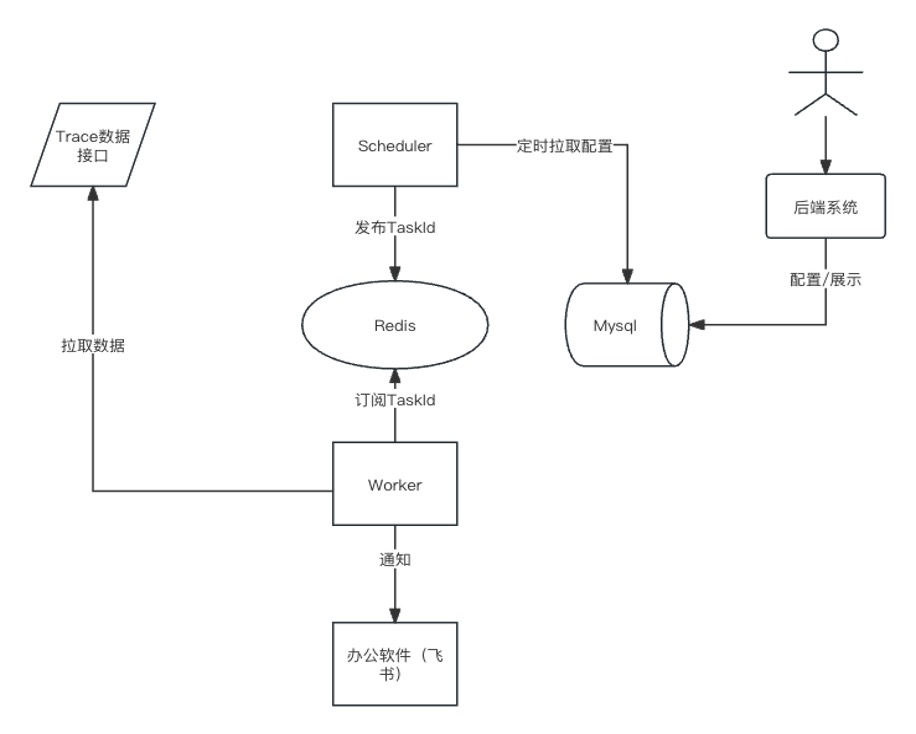
\includegraphics[width=5in]{figure/chapter4/告警平台总体详细设计.jpg}
  \caption{告警平台总体详细设计}\label{gaojingzongti}
\end{figure}

正如上图所示,告警平台的流程是前端用户提交基本配置、指标配置、检测配置元信息给后端系统建立定时任务,将任务记录持久化到Mysql,Scheduler模块定时拉取未处理的记录给Redis中的消息队列,Worker组件对任务进行具体的执行。首先从Trace接口拉取数据,然后根据告警规则进行检测。若有异常也会根据配置信息对用户进行通知。下面展示一下元数据配置信息,分别是告警平台基本配置、告警平台指标配置、告警平台检测配置。

\begin{figure}[htb]
  \centering
  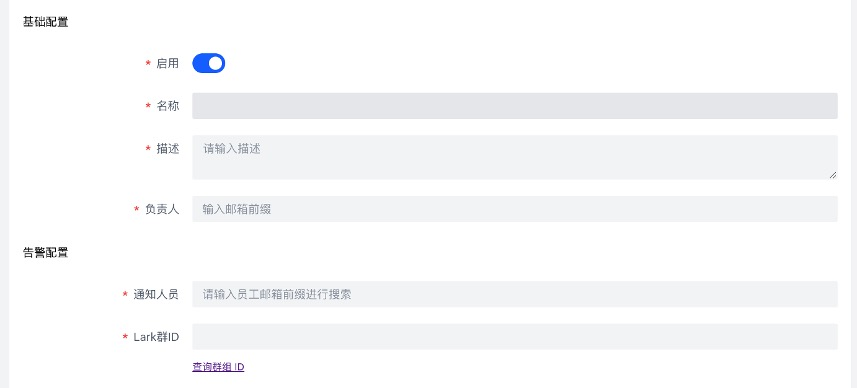
\includegraphics[width=5in]{figure/chapter4/告警平台基本配置.jpg}
  \caption{告警平台基本配置}\label{gaojingjiben}
\end{figure}

如\ref{gaojingjiben}所示启用状态默认为开启,可以根据需要进行关闭,设置为"开启"后,配置完立刻会运行。名称根据业务背景命名,中英文不限。描述简述监控策略与告警阈值等信息,拥有监控配置的编辑与删除权限,可添加多人,建议将自己加上,否则创建后自己无法操作。通知人员告警信息接收人,可添加多人。

\begin{figure}[htb]
  \centering
  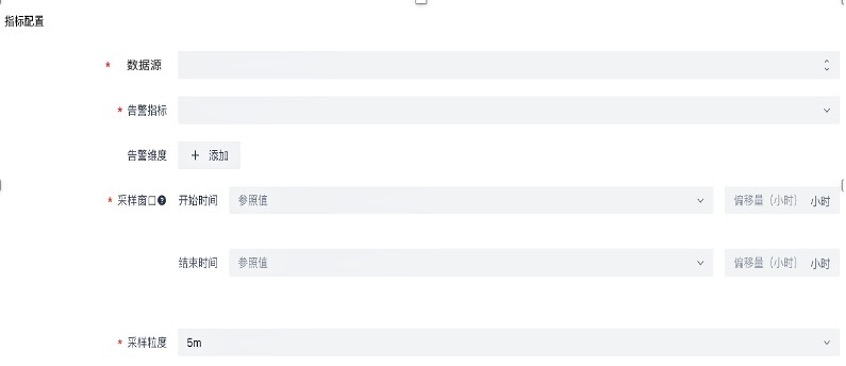
\includegraphics[width=5in]{figure/chapter4/告警平台指标配置.jpg}
  \caption{告警平台指标配置}\label{gaojingzhibiao}
\end{figure}

图\ref{gaojingzhibiao}中数据源是指需要查询Trace系统下的哪些数据,比如说抖音下的点播数据,因此需要指明数据来源。告警指标是指所选择的数据源中包含的指标。告警维度是选取指标相应维度,填写检测维度取值,有多个取值可用英文逗号分隔。采样窗口\cite{hasanin2019severely}是指指标数据拉取的时间窗口,采样的数据作为后台检测算法的输入。开始/结束时间:采样窗口上下界的基准时间,今天的话就是任务执行当天零点;此刻就是任务执行时刻。采样粒度是采样指标数据的聚合粒度(时间GroupBy区间长度)。
\begin{figure}[htb]
  \centering
  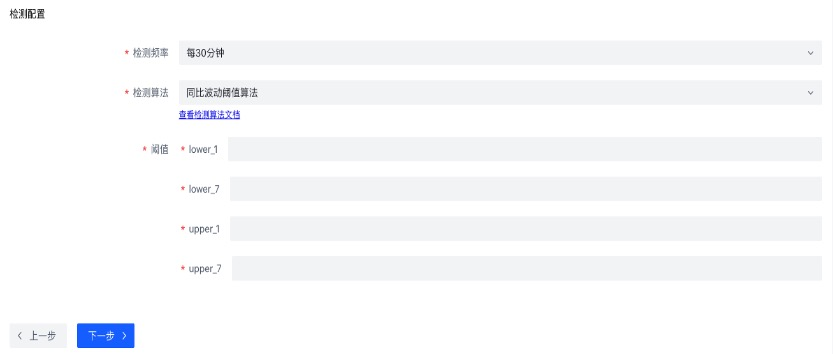
\includegraphics[width=5in]{figure/chapter4/ 告警平台检测配置.jpg}
  \caption{告警平台检测配置}\label{gaojingjice}
\end{figure}
检测频率是监控任务的运行频率检测算法分为静态阈值算法和同比算法。在需求分析时对两者进行了分析,这里就不再做解释。其实对于检测算法也提供了采用机器学习来进行,例如常见的算法有卷积自编码器 (Convolutional Reconstruction Autoencoder Model)、孤立森林 (Isolation Forest Model)、XGBoost 预测等等。检测出异常将以卡片的形式告知用户,如图\ref{gaojingkapian}所示:

\begin{figure}[htbp]
  \centering
  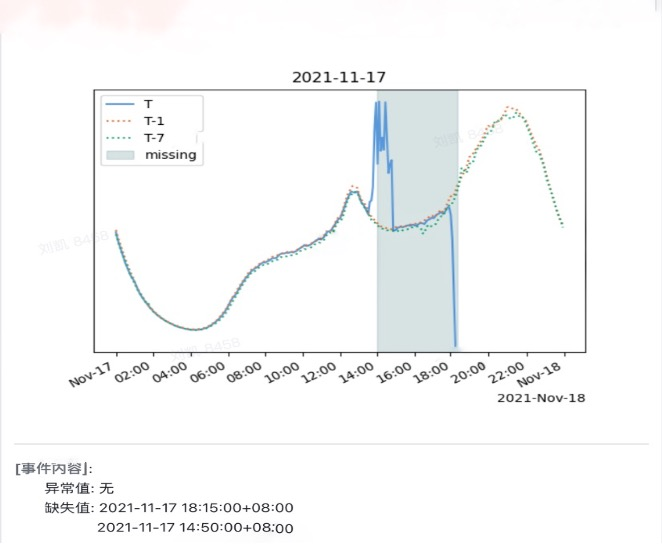
\includegraphics[width=5in]{figure/chapter4/告警通知卡片.jpg}
  \caption{告警通知卡片}\label{gaojingkapian}
\end{figure}

以上就是对告警配置信息的介绍,后端会将其保存到Mysql中。告警模块Worker组件负责具体的执行。生产者即Scheduler组件负责将从Mysql中扫描到的数据进行解析构造成配置对象,并对其进行校验,将其放入消息队列。消费者即为Worker组件,消费者获取到配置信息后,会对规则其进行解析,规则的JSON结构记录了前端提交的配置信息。它的具体结构如下图\ref{peizhijiexi}所示:
\begin{figure}[htbp]
  \centering
  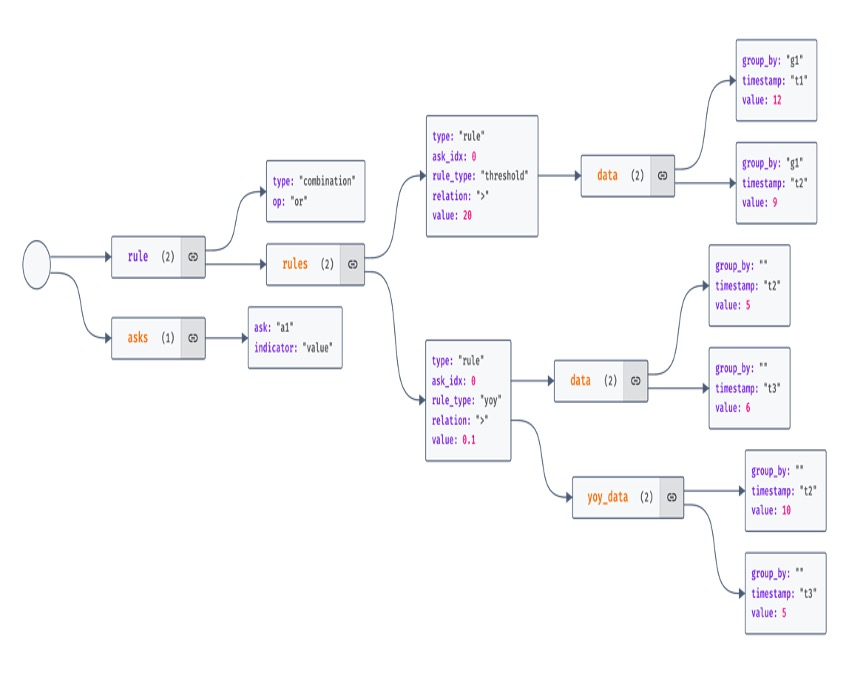
\includegraphics[width=5in]{figure/chapter4/配置信息解析结构.jpg}
  \caption{配置信息解析结构}\label{peizhijiexi}
\end{figure}

上图JSON结构中的asks代表数据源信息,rule\_type代表具体规则算法,threshold为静态阈值,yoy为同比算法。GroupBy是指对某个指标字段进行分组聚合,类似于SQL中的GroupBy。Rule(2)就说明一个配置杂糅了两个规则,这两个规则采用了不同的算法进行检测,最终的异常结果是两者结果的与或关系。

如果规则是一个简单的规则,则它直接返回规则的异常值和异常点。否则即为组合规则,Worker需递归地处理每个子规则,并使用子规则的检测结果来确定组合规则的检测结果,并根据规则的“或”与“与”关系来确定是否存在异常。图\ref{jianceliuchengshangxia}为检测的具体执行流程:
\newpage
 \begin{figure}[h!]
  \centering
  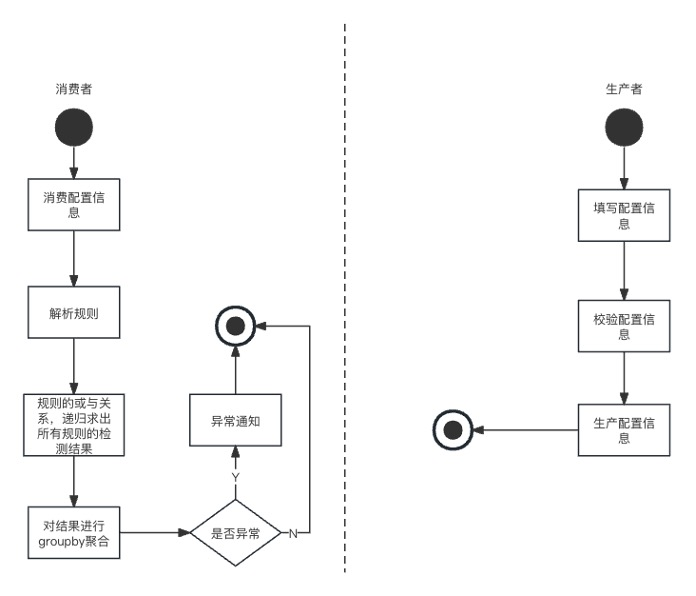
\includegraphics[width=5in]{figure/chapter4/检测流程及上下文.jpg}
  \caption{检测流程及上下文}\label{jianceliuchengshangxia}
\end{figure}


以上对告警平台各个组件的功能进行了详细介绍,下面将从实现的角度对该模块进行类图展示:

\begin{figure}[htbp]
  \centering
  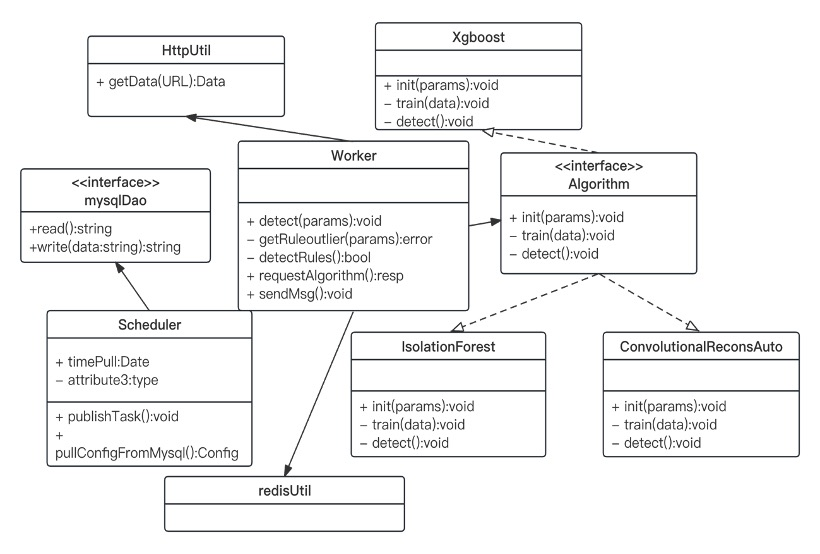
\includegraphics[scale=0.3888]{figure/chapter4/告警平台模块类图.jpg}
  \caption{告警平台模块类图}\label{gaojingclass}
\end{figure}
Worker类作为整个模块核心进行调度,通过httpUtil拉取Trace数据进行异常检测,算法以接口的形式暴露给Worker组件。下面再对检测算法进行详细分析,首先调研了国内外企业和机构几个模型,如表\ref{suanfadiaoyan}所示:
\begin{table}[h!] 
\centering  
\caption{检测模型调研分析}  
\scriptsize % 使用\scriptsize来进一步减小字体大小  
\begin{tabular}{lccccc}  
\hline  
对比维度 & 百度运维部 & 滴滴出行 & Metis & 阿里巴巴 & 华为消费者BG  \\ \hline 
年份/地点 & 2017年9月/北京 & 2017年9月/北京 & 2017年8月-至今 & 2018年9月/上海 & 2018年9月/上海  \\ \hline  
整体技术框架 & 先分类,再检测 & 先分类,再检测 & 直接检测,分类特征 & 先分类,再检测 & 单条时间序列建模  \\ \hline  
机器学习模型 & \begin{tabular}[c]{@{}c@{}}同环比模型\\ 阈值模型\end{tabular} & \begin{tabular}[c]{@{}c@{}}同环比模型\\ 阈值模型\\ 趋势模型\end{tabular} & \begin{tabular}[c]{@{}c@{}}无监督模型\\ 有监督模型\\ 控制图理论\\ 多项式拟合\\ XGBoost\end{tabular} & \begin{tabular}[c]{@{}c@{}}同环比模型\\ 阈值模型\\ Holt-Winters\end{tabular} & 无监督模型 \\ \hline  
深度学习(单条) & 无 & 无 & 自编码器,VAE & VAE & 无 \\ \hline  
深度学习(海量) & 无 & 无 & DNN,LSTM & 无 & 无  \\ \hline  
单调性/定时任务 & 无 & 无 & \begin{tabular}[c]{@{}c@{}}线性拟合/\\ 周期性识别算法\end{tabular} & 无 & 无  \\ \hline  
开源 & 只有打标工具 & 无 & \begin{tabular}[c]{@{}c@{}}打标工具\\ 无监督模型\\ 有监督模型\end{tabular} & 无 & 无  \\ \hline  
\end{tabular}  
\label{suanfadiaoyan}
\end{table}

对于简单阈值设置和同比阈值波动设置上文已经进行了介绍,下面分别对卷积自编码器、孤立森林和Xgboost算法进行详解的介绍。

卷积自编码器 (Convolutional Reconstruction Autoencoder Model)\cite{} 基于一条很长的时间序列,可以提取它的很多子序列,从而构造出很多的片段序列。
  \begin{figure}[h!]
  \centering
  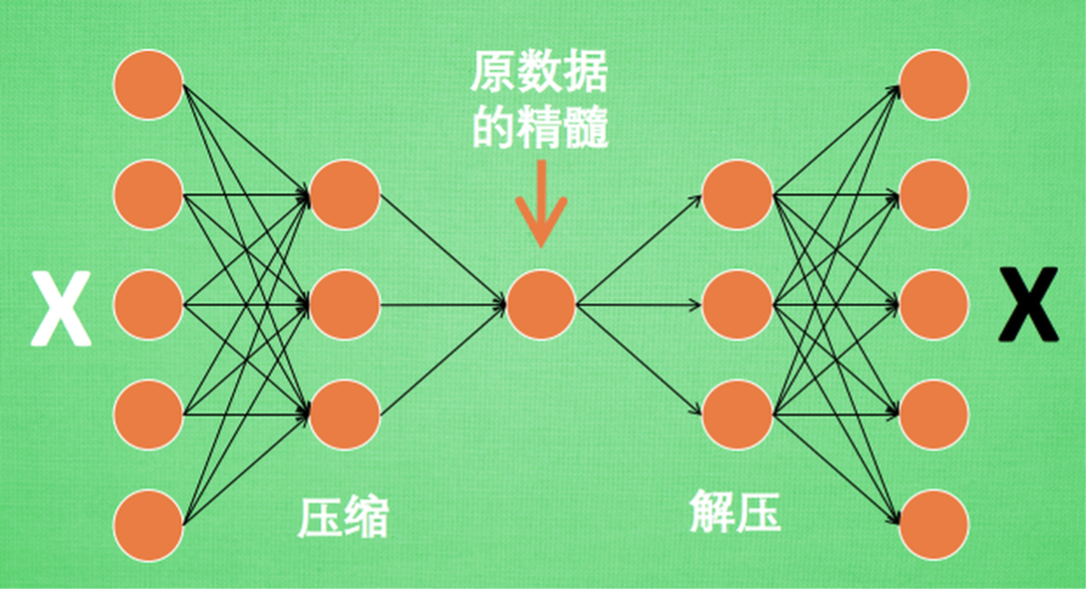
\includegraphics[scale=0.9]{figure/chapter4/卷积自编码器原理.png}
  \caption{卷积自编码器原理}\label{juanjiyuanli}
\end{figure}

这些片段序列就可以形成自编码器的输入数据,而自编码器是模拟一个恒等变换,因此它会把有异常的点尽量磨平,而正常的点则保持原样。所以,通过大量子片段来进行训练数据的输入,自编码器就能够得到一个较为合理的权重。得到了一个训练好的自编码器之后,对于任何一个子片段,都可以重构出一个新的片段。

训练autoencoder重构时序数据,使用MSE Loss训练,通过训练确定 MAE作为还原误差的阈值,预测时来判断当前数据是否异常。适用于有较为稳定训练数据的情况,同时要保证数据整体的平稳性。输入及重构后的例子:

  \begin{figure}[htbp]
  \centering
  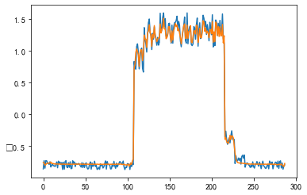
\includegraphics[scale=0.9]{figure/chapter4/卷积自编码器实际检测案例.png}
  \caption{卷积自编码器实际检测案例}\label{juanjiyuanlianli}
\end{figure}

孤立森林 (Isolation Forest Model)是一个基于Ensemble的快速异常检测方法~\cite{杨晓晖2019基于多粒度级联孤立森林算法的异常检测模型},具有线性时间复杂度和高精准度。

\begin{figure}[htbp]
  \centering
  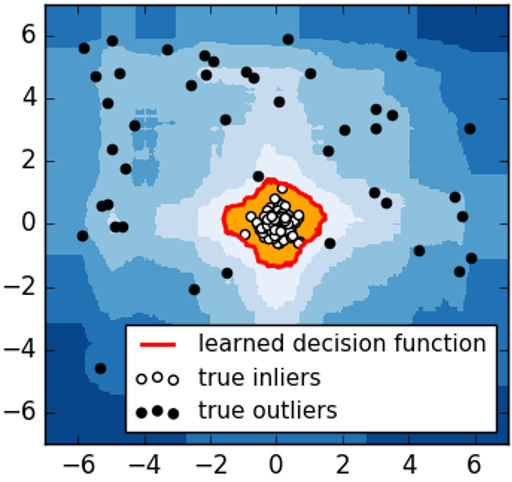
\includegraphics[scale=0.85]{figure/chapter4/孤立森林原理图.png}
  \caption{孤立森林原理图}\label{gulisenlin}
\end{figure}

iForest适用于连续数据(Continuous numerical data)的异常检测,将异常定义为“容易被孤立的离群点 (more likely to be separated)”——可以理解为分布稀疏且离密度高的群体较远的点。用统计学来解释,在数据空间里面,分布稀疏的区域表示数据发生在此区域的概率很低,因而可以认为落在这些区域里的数据是异常的。
孤立森林通过多颗树形成森林来判定是否有异常点,这种方法很有效,但是并不总是有用的,比如说数据的分布不是沿着特征轴,而是随意分布,或者流型分布,就需要选择别的方式了。

\begin{figure}[htbp]
  \centering
  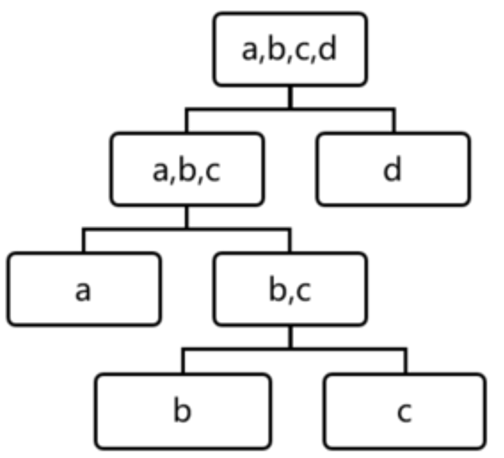
\includegraphics[scale=0.8]{figure/chapter4/森林判定异常点.png}
  \caption{森林判定异常点}\label{senlinpanding}
\end{figure}

XGBoost是Extreme GradientBoosting的缩写,是一种高效的随机梯度提升的实现~\cite{赵洪山2019应用深度自编码网络和}。随机梯度提升算法(或者叫gradient boosting machines ortree boosting)是一种强大的机器学习技术,在很多有挑战的机器学习问题上,表现的非常好甚至是最好。它是一个决策树算法的集成,其中新树可以对模型中已有树的结果进行修正。

该算法思想就是不断地添加树,不断地进行特征分裂来生长一棵树,每次添加一个树,其实是学习一个新函数,去拟合上次预测的残差。当我们训练完成得到k棵树,我们要预测一个样本的分数,其实就是根据这个样本的特征,在每棵树中会落到对应的一个叶子节点,每个叶子节点就对应一个分数,最后只需要将每棵树对应的分数加起来就是该样本的预测值。

\begin{figure}[htbp]
  \centering
  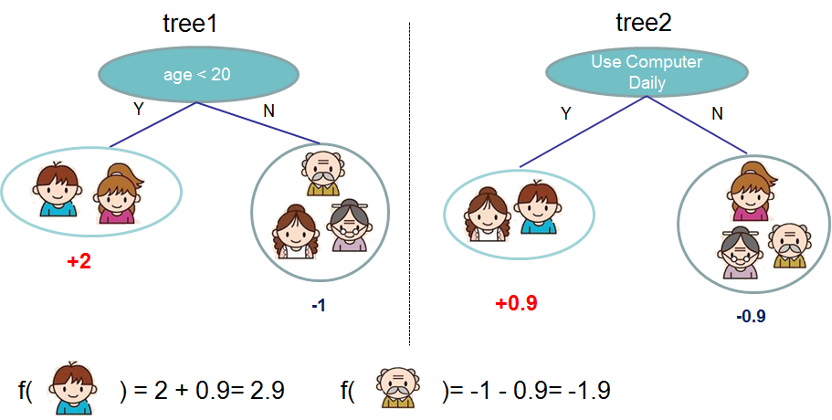
\includegraphics[scale=0.8]{figure/chapter4/XGBoost原理图.png}
  \caption{XGBoost原理图}\label{xgboostyuanli}
\end{figure}
\newpage
对于1D的时序数据,需要进一步处理,如提取特征、滑动窗口等方式,使之成为有监督学习的输入。对于一个时间序列数据的特征提取例子:
    \begin{figure}[htbp]
  \centering
  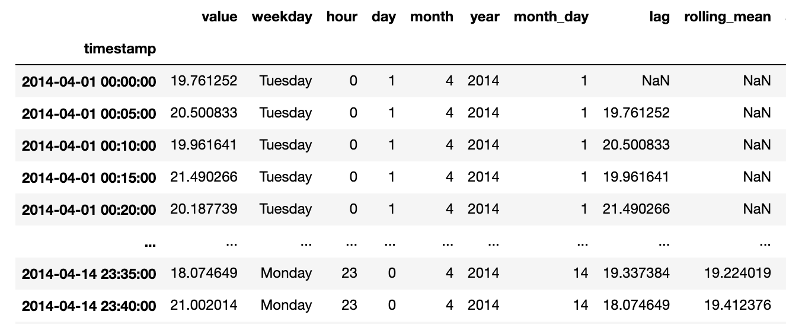
\includegraphics[scale=0.8]{figure/chapter4/XGBoost演示效果测试数据.png}
  \caption{XGBoost演示效果测试数据}\label{xgboostxiaoguceshiju}
\end{figure}

预测的效果图如下图\ref{xgboostxiaoguo},对于预测得到的点,可以设置一个波动阈值,以此来判断当前的实际值是否偏离正常值预期。
    \begin{figure}[htbp]
  \centering
  \includegraphics[scale=0.8]{figure/chapter4/XGBoost预测效果图.png}
  \caption{XGBoost预测效果图}\label{xgboostxiaoguo}
\end{figure}
\newpage
\subsection{流媒体埋点查询系统接口设计}
Trace系统中接口分为两种,分别是Http接口和RPC接口。Http接口用于前后端之间或者系统和网关之间的通信。系统内部以Kitex进行组织,上下游服务之间的调用以Thrift格式进行通信。
   
在系统中Http接口存在三个,分别是实时查询接口、离线查询接口、字段
管理接口。前端原型图如下图\ref{chaxunyuanxing}所示:
\begin{figure}[htbp]
  \centering
  \includegraphics[scale=0.3]{figure/chapter4/查询界面原型图.jpg}
  \caption{查询界面原型图}\label{chaxunyuanxing}
\end{figure}

下面将以表格的形式对三个接口进行设计:

\begin{longtable}{p{2cm}p{3cm}p{2cm}p{2cm}p{4cm}} 
\caption{API table for /live\_trace/v1/mget post} 
\toprule  
\textbf{Category} & \textbf{Parameter} & \textbf{Type} & \textbf{Default} & \textbf{Comment} \\ \midrule  
\endfirsthead  
  
\hline  
\toprule  
\textbf{Category} & \textbf{Parameter} & \textbf{Type} & \textbf{Default} & \textbf{Comment} \\ \midrule  
\endhead  
\multirow{7}{*}{\textbf{Request}} & {1} Namespace & string & & 标识数据源信息 \\  
& {2} Start & Int64 & & 检索起始时间 \\  
& {3} End & Int64 & & 检索结束时间 \\  
& {4} Limit & Int64 & 100 & 分页查询条数 \\  
& {5} Offset & Int64 & 0 & 分页查询偏移量 \\  
& {6} Filter & []*Filter & Nil & 筛选条件 \\  
& {  6.1} Field & string & & 筛选字段名称 \\  
& {  6.2} Op & string & & 筛选条件符 \\  
& {  6.3} Value & string & Nil & 筛选字段值 \\  
& {7} Interval & Int64 & Auto & 时间间隔长度 \\  
& {8} LucenceString & String & & Lucence表达式 \\
\multirow{6}{*}{\textbf{Response}} & {1} List & []map[string]interface{} & & 查询BMQ全量数据 \\  
&{2} TimeBarInter & Int64 & 15s & 动态时间分组间隔 \\  
&{3} TaskId & Int64 & & 任务Id号 \\  
& \multirow{1}{*}{4 TimeBars} & \multirow{1}{*}{[]*TimeBar} & \multirow{1}{*}{nil} & \multirow{1}{*}{每个时间分组的描述} \\ 
& {  4.1} TimeKey & Int64 & nil& 返回消息的起始时间 \\  
& {  4.2} cnt & Float64 &0& 分组内数据数量 \\  
\bottomrule  
\end{longtable} 
\vspace{1.5cm} % 在这里添加空隙





\begin{table}[htbp]  
\centering  
\caption{API table for live\_trace/v1/offlineSubmit post} 
{
\begin{tabular}{p{2cm}p{3cm}p{2cm}p{2cm}p{4cm}}  
\toprule  
\textbf{Category} & \textbf{Parameter} & \textbf{Type} & \textbf{Default} & \textbf{Comment} \\ \midrule  
\multirow{7}{*}{\textbf{Request}} & {1} Namespace & string & & 标识数据源信息 \\  
& {2} Start & Int64 & & 检索起始时间 \\  
& {3} End & Int64 & & 检索结束时间 \\  
& {4} Limit & Int64 & 100 & 分页查询条数 \\  
& {5} Offset & Int64 & 0 & 分页查询偏移量 \\  
& {6} Filter & []*Filter & Nil & 筛选条件 \\  
& {  6.1} Field & string & & 筛选字段名称 \\  
& {  6.2} Op & string & & 筛选条件符 \\  
& {  6.3} Value & string & Nil & 筛选字段值 \\  
& {7} Interval & Int64 & Auto & 时间间隔长度 \\  
& {8} LucenceString & String & & Lucence表达式 \\ \cmidrule{2-5}  
\multirow{3}{*}{\textbf{Response}} & {1} jobId & Int64 & & 任务id号\\ &{2} Code & Int & 200 & 动态时间分组间隔 \\  
&{3} TaskId & Int64 & & 任务Id号 \\  
\bottomrule  
\end{tabular}  
\label{table:offlineSubmit}
}
\end{table}  

\begin{table}[htbp]  
\centering  
\caption{API table for live\_trace/v1/addFields post} 
{
\begin{tabular}{p{2cm}p{3cm}p{2cm}p{2cm}p{4cm}} 
\toprule  
\textbf{Category} & \textbf{Parameter} & \textbf{Type} & \textbf{Default} & \textbf{Comment} \\ \midrule  
\multirow{7}{*}{\textbf{Request}}
& {1} Namespace & string & & 标识数据源信息 \\  
& {2} FieldName & string & & 字段名称 \\  
& {3} FieldSourceId & Int64 & & 字段来源 \\  
& {4} FieldOwner & string & 100 & 字段创造者 \\  
& {5} FieldType & string & 0 & 字段类型 \\  
& {6} FieldDesc & string & Nil & 字段描述 \\  
& {7} Indexed & Bool & False & 是否为索引字段 \\  
\cmidrule{2-5}  
\multirow{3}{*}{\textbf{Response}} & {1} Code & Int &0&\begin{tabular}[c]{p{4cm}} 0: Successful insertion; -1: useless insertion;  -2: insert failed; -3: field quantity limit exceeded, \end{tabular}\\ &{2} Message & string & 0 & 任务运行信息 \\  
\bottomrule  
\end{tabular}  
}
\label{table:offlineSubmit}
\end{table}  
\newpage
\vspace{-1.5cm} % 在这里添加空隙
BMQ查询服务应该与本系统隔离,因此单独封装了BMQ服务对外提供服务。后端系统与BMQ服务之间的通信是使用Kitex thrift进行通讯,上下游需定义好通讯接口。Thrift提供跨语言的服务框架,这种跨语言主要体现在它对多种语言的编译功能的支持,用户只需要使用IDL描述好接口函数,只需要一条简单的命令,Thrift就能够把按照IDL格式描述的接口文件翻译成各种语言版本。
如\ref{tab:mycode}表所示具体介绍下BMQ服务请求thrift格式:

\begin{lrbox}{\mylistingboxOne}  
\begin{lstlisting}[language=Java]  
struct TStatus {
  1:i32 code;
  2:string msg;
}
struct TConfig {
  1:i32 limit = 100; //limit records, defalut is 100
  2:i32 maxBytes = 10000000; //max bytes, default is 10M
}
struct TFilter {
  1:string type; //support:equal、prefix、suffix、regex、range
  2:string key;
  3:string expression;
}

\end{lstlisting}  
\end{lrbox} 

\begin{table}[h]  
\caption{BMQ的thrift的格式}  
\label{tab:mycode}  
\usebox{\mylistingboxOne}  
\end{table}  

\begin{lrbox}{\mylistingboxTwo}  
\begin{lstlisting}[language=Java]  
struct TQuery {
  1:required string cluster;
  2:required string topic;
  3:required string partitionKey;
  4:required map<string, string> indexKey;
  5:list<TFilter> filters;
  6:TConfig config;
  7:TContext context;
}
struct TRecord {
  1:i64 offset;
  2:string value;
}
struct TPartitionRecord {
  1:i32 partition;
  2:list<TRecord> records;
}
struct TRemainRecords {
  1:i32 partition;
  2:list<i64> offsets;
}
struct TResult {
  1:TStatus status;
  2:list<TPartitionRecord> partitionRecords;
  3:TContext context;
}
service TQueryService {
  TResult Query(1:TQuery query);
} 
\end{lstlisting}  
\end{lrbox} 
\begin{table}[h]  
\usebox{\mylistingboxTwo}  
\end{table}  



上面的通信协议考虑到了BMQ通信的结果状态、以及分批查询时应可以判断是否还会存在下一批数据,以及剩余数据在消息队列中的offset。每一批数据都有数量和大小的限制,超出限制则丢弃。查询必须指明Topic,以及要点查数据的partitionKey。BMQ支持多维查询,需要对统一个Value做多维索引,即多个IndexKey定位同一个记录,但对于同一个IndexKey的数量不要太多,否则会影响查询速度,应在1000个以内。Query也提供了内置的Filter和自定义Filter功能,以便过滤不需要的数据,提升查询效率。以上功能在thrift文件中都有涉及。

\section{流媒体埋点查询系统数据库设计}
系统中用到了Mysql、ElasticSearch、BMQ INDEX三种持久化数据库。这三者分别属于关系型数据库、文档型数据库、KV消息队列。因此,对三者的设计也有着不同的设计要求和考虑的方向。接下来将对三者进行逐一详细设计。

系统中使用关系型数据库存储离线查询任务记录、埋点数据字段、告警任务记录、告警事件记录、pullData数据拉取记录。除了埋点数据字段表,其他都是持久化元数据表。数据模型设计如下图\ref{ergraph}所示:
\begin{figure}[htbp]
  \centering
  \includegraphics[scale=1]{figure/chapter4/数据库表实体关系图.png}
  \caption{数据库表实体关系图}\label{ergraph}
\end{figure}

下面以表格的形式详细展示数据表的数据结构和索引信息。

1)	离线查询表

如表\ref{offlineSearch}描述了id、namespace、job\_id、job\_status 、owner、sql\_query、result\_url、origin\_query、created\_time、updated\_time共10个字段。还定义了主键索引id、基于job\_id字段来提高job\_id字段的查询速度的普通索引idx\_jobid。基于job\_status字段的前191个字符来提高job\_status字段前缀的查询速度的前缀索引idx\_jobstatus。

\begin{table}[h] 
\centering % 这个命令会使表格居中
\caption{离线查询表}
\begin{tabular}{|c|c|c|}  
\hline  
字段 & 类型 & 描述 \\ \hline  
id & bigint & 唯一标识 \\ \hline  
namespace & varchar(255) & data source namespace \\ \hline  
job\_id & varchar(255) & tqs job id \\ \hline  
job\_status & varchar(255) & tqs job status \\ \hline  
owner & varchar(255) & job owner \\ \hline  
sql\_query & text & sql query \\ \hline  
result\_url & text & tqs result \\ \hline  
origin\_query & text & origin query \\ \hline  
created\_time & Int & create time \\ \hline  
updated\_time & Int & update time \\ \hline  
\multicolumn{2}{|c|}{\multirow{2}{*}{索引信息}} & KEY `idx\_jobid` (`job\_id`) \\   
\cline{3-3}  
\multicolumn{2}{|c|}{} & KEY `idx\_jobstatus` (`job\_status`(191)) \\ \hline  
\end{tabular} 
\label{offlineSearch}  
\end{table}

\newpage
2)	埋点数据信息表
如下表\ref{maidiandatatable}描述了id、namespace、indexed、hot、field\_desc、expire\_in、field\_owner、field\_source\_id、field\_type、created\_time、updated\_time、operator共13个字段。
tracking\_field\_ns\_field\_unique\_index (namespace,field\_name)是一个唯一索引,用于确保在相同的namespace下不会有重复的field\_name,维护数据的完整性和一致性。tracking\_field\_namespace\_indexed\_index (namespace,indexed)是复合索引,基于namespace和indexed字段构建。它可以优化基于这两个字段的查询性能。tracking\_field\_namespace\_hot\_index (namespace,hot)也是一个复合索引,基于namespace和hot字段构建。它可以优化基于这两个字段的查询性能。

\begin{longtable}[htbp]   
\caption{埋点数据信息表}
\hline  
\textbf{字段} & \textbf{类型} & \textbf{描述} 
\endfirsthead  

\textbf{字段} & \textbf{类型} & \textbf{描述} 
\endhead  
id & bigint & 字段唯一ID \\ \hline  
namespace & varchar(64) & 字段所在BMQ的namespace \\ \hline  
indexed & tinyint(1) & 是否可以用于筛选 \\ \hline  
hot & tinyint(1) & 是否热门字段 \\ \hline  
field\_desc & varchar(2048) & 字段描述信息 \\ \hline  
field\_name & varchar(128) & 字段名称 \\ \hline  
expire\_in & int(10) & 任务ID \\ \hline  
field\_owner & varchar(2048) & 任务快照信息 \\ \hline  
field\_source\_id & int & 上报方id \\ \hline  
field\_type & varchar(32) & 字段类型 \\ \hline  
created\_time & bigint & 字段创建时间 \\ \hline  
updated\_time & bigint & 字段更新时间 \\ \hline  
operator & varchar(32) & 操作人 \\ \hline  
\multicolumn{2}{|c|}{\multirow{4}{*}{索引信息}} & PRIMARY KEY(`id`) \\ \cline{3-3}  
\multicolumn{2}{|c|}{} & KEY`tracking\_field\_ns\_field\_unique\_index` (`namespace`,`field\_name`) \\ \cline{3-3}  
\multicolumn{2}{|c|}{} & KEY`tracking\_field\_namespace\_indexed\_index`(`namespace`,`indexed`) \\ \cline{3-3}  
\multicolumn{2}{|c|}{} & KEY `tracking\_field\_namespace\_hot\_index` (`namespace`,`hot`) \\ \hline  
\end{tabular}  
\label{maidiandatatable}

\end{table}  

\newpage
3)	告警任务记录表

如下表\ref{gaojingrecord}描述了id、uuid、name、description、status、 task\_type、detail、owner、created\_at、updated\_at共10个字段。此外,这个表还定义了几个索引。基于id字段的主键索引,基于uuid字段的唯一索引,从而确保这个字段的值在整个表中是唯一的。基于task\_type和updated\_at字段的复合索引,基于name字段的单字段索引。

\begin{table}[htbp]  
\centering  
\scriptsize
\caption{告警任务记录表}
\begin{tabular}{|c|c|c|}  
\hline  
字段 & 类型 & 描述 \\ \hline  
id & bigint & 主键 \\ \hline  
uuid & varchar(40) & 对外展示的id \\ \hline  
name & varchar(255) & 任务的名称 \\ \hline  
description & text & 任务的描述 \\ \hline  
status & varchar(255) & 任务的状态 \\ \hline  
task\_type & varchar(255) & 任务的类型,默认为outlier \\ \hline  
detail & text & 任务的配置信息 \\ \hline  
owner & text & 任务管理员 \\ \hline  
created\_at & datetime & 创建时间 \\ \hline  
updated\_at & datetime & 修改时间 \\ \hline  
\multicolumn{2}{|c|}{\multirow{4}{*}{索引信息}} & PRIMARY KEY (`id`) \\ \cline{3-3}  
\multicolumn{2}{|c|}{} & KEY `uniq\_timeseriestask\_uuid` (`uuid`) \\ \cline{3-3}  
\multicolumn{2}{|c|}{} & KEY`idx\_sniper\_config\_updated\_at`(`task\_type`(191),`updated\_at`) \\ \cline{3-3}  
\multicolumn{2}{|c|}{} & KEY `idx\_sniper\_name` (`name`) \\ \hline  
\end{tabular}  
\label{gaojingrecord}
\end{table} 

4)	告警事件通知记录表

表\ref{gaojingshijiantongzhitable}描述了id、uuid、message\_id、notification\_type、task\_uuid、receiver、detail、created\_at共9个字段。此外,表定义还包括以下索引,主键索引(基于id字段)、唯一索引uniq\_notificationrecord\_uuid(基于uuid字段),确保通知记录的uuid在整个表中是唯一的。

\begin{table}[h] 
\centering
\small
\caption{告警事件通知记录表}
\begin{tabular}{|c|c|c|}  
\hline  
字段 & 类型 & 描述 \\ \hline  
id & int & 主键 \\ \hline  
uuid & varchar(40) & 通知记录 \\ \hline  
message\_id & varchar(128) & 通知消息的id \\ \hline  
notification\_type & varchar(64) & 通知消息的类型 \\ \hline  
task\_uuid & varchar(40) & 通知消息的任务id \\ \hline  
receiver & varchar(128) & 通知消息的接收人 \\ \hline  
event\_id & varchar(40) & 通知消息的事件聚合id \\ \hline  
detail & text & 通知消息的详情 \\ \hline  
created\_at & datetime & 通知消息的创建时间 \\ \hline  
\end{tabular}  
\label{gaojingshijiantongzhitable}
\end{table}

5)	pullData数据拉取记录表

表\ref{pulldatatable}描述了pullData数据拉取记录表存储任务配置的信息。表结构包括id、name、description、status、task\_type、detail、owners、visibility(表示任务的可见性等级如private、public等)、create\_time、update\_time共10个字段。 


\begin{table}[h] 
\centering
\small
\caption{pullData数据拉取记录表}
\begin{tabular}{|c|c|c|}  
\hline  
字段 & 类型 & 描述 \\ \hline  
id & bigint & 主键 \\ \hline  
name & varchar(100) & 任务的名称 \\ \hline  
description & text & 任务的描述 \\ \hline  
status & varchar(255) & 任务状态:delete;close;open \\ \hline  
task\_type & varchar(255) & 任务的类型,默认为outlier \\ \hline  
detail & text & 任务的配置信息 \\ \hline  
owner & text & Owners \\ \hline  
visibility & varchar(200) & 可见性等级:private;public \\ \hline  
created\_at & timestamp & 创建时间 \\ \hline  
updated\_at & timestamp & 修改时间 \\ \hline  
\end{tabular}  
\label{pulldatatable}
\end{table}

ElasticSearch用来保存少量的埋点索引字段,这样做使得ElasticSearch变得更加轻量级,为了适配当前超大数据量和写入吞吐量的情况,配置如下表\ref{tab:esconfig}所示:
routing.allocation.total\_shards\_per\_node限制了每个节点上允许的最大分片数。它被设置为2,意味着每个Elasticsearch节点上最多只能有两个分片,用来防止节点因为过多的分片而变得过于繁忙。refresh\_interval是Elasticsearch的刷新间隔,设置为"120s"表示每120秒刷新一次索引。刷新操作使得新的文档可以被搜索到,但也会产生一些开销。number\_of\_shards是索引的分片数\cite{wei2020optimization},设置为965用来实现分布式搜索和扩展性的基本单位。translog是事务日志的设置。durability设置为"async"表示异步写入事务日志可以提高写入性能但可能会增加数据丢失的风险。sync\_interval设置为"60s"表示每60秒同步一次事务日志到磁盘。allocation.max\_retries控制了在分配失败时尝试重新分配分片的最大次数。number\_of\_replicas是索引的副本数,设置为0表示没有副本。

\begin{lrbox}{\esconfigbox}  
\begin{lstlisting}[language=Java]  
{   "index": {
        "routing": {
            "allocation": {
                "total_shards_per_node": 2
            }
        },
        "refresh_interval": "120s",
        "number_of_shards": 965,
        "translog": {
            "durability": "async",
            "sync_interval": "60s"
        },
        "allocation.max_retries": 500,
        "number_of_replicas": 0}
}
\end{lstlisting}  
\end{lrbox} 

\begin{table}[h]    
\caption{ElasticSearch setting配置信息}  
\label{tab:esconfig}  
\usebox{\esconfigbox}  
\end{table}  



为了适配实时变化的索引字段,ElasticSearch应开启动态索引功能,这就要求写入的数据类型需进行Mapping映射,由于都是自定义的,具体案例如下表\ref{tab:esindexconfig}所示:

Elasticsearch的映射配置的一部分,用于定义索引中字段的动态模板。动态模板允许你根据字段的类型或名称来自动应用特定的映射配置。在这个例子中,有三个动态模板:

1)	integers模板:当Elasticsearch遇到一个新的字段,并且它的数据类型被识别为long时,这个模板会被应用。

2)	strings模板:当Elasticsearch遇到一个新的字符串字段时,这个模板会被应用。模板指定该字段的类型应该被映射为keyword,该字段将被视为一个精确值字段,而不是一个全文搜索字段。

\begin{lrbox}{\esconfigindexbox}  
\begin{lstlisting}[language=Java]  
{
    "dynamic": true,
    "dynamic_templates": [
        {
            "integers": {
                "mapping": {
                    "type": "long"
                },
                "match_mapping_type": "long"
            }
        },
        {
            "strings": {
                "mapping": {
                    "type": "keyword"
                },
                "match_mapping_type": "string"
            }
        }
      ]
}
\end{lstlisting}  
\end{lrbox} 

\begin{table}[h]   
\caption{ElasticSearch动态索引配置信息}  
\label{tab:esindexconfig}  
\usebox{\esconfigindexbox}  
\end{table}  

由于ElasticSearch的同步写入压力巨大,为了降低同步处理的事件,将数据写入转为后台异步执行。因此设计架构变为数据先流入Kafka消息队列,然后由Beats同步工具将数据流入ElasticSearch中。Beats配置文件中应指明数据的来源和去处。以及对Kafka和ElasticSearch的配置。


接下来继续介绍BMQ INDEX的配置,它分为消息队列和索引两部分,因此首先需定义好消息队列中消息的Schema,然后依赖消息结构构造索引。首先应弄懂两个概念Partition Key和Index Key。Partition Key为消息的分片Key,此Key可以通过分区策略确定数据存在了哪个分区中。Index Key为一条消息的索引,业务可通过DDL指定相关Index Key,将会根据此Key建立索引文件。在Trace系统实际设计中将Partition Key和Index Key都指定为app\_id:device\_ip,app\_id标识了数据是由哪个应用产生的,device\_id标识了产生数据的设备。

对于消息Schema来讲,目前BMQ中的数据格式可以由PB格式和Json两种格式构成,下面以JSON为例,消息结构如下表\ref{tab:bmqSchema}所示,
\begin{lrbox}{\bmqSchema}  
\begin{lstlisting}[language=Java]  
{
    "type": "object",
    "properties": {
        "partitionKey": {
            "type": "string"
        },
        "clusteringKey": {
            "type": "string"
        },
        "value": {
            "type": "string"
        }
    }
}
\end{lstlisting}  
\end{lrbox} 
\begin{table}[h]   
\caption{BMQ数据Schema信息}  
\label{tab:bmqSchema}  
\usebox{\bmqSchema}  
\end{table}  
其中partitionKey上文已经介绍过,clusteringKey为写入时间戳,用于做范围扫描,value是经过压缩编码后的数据。在此基础上,将对以上格式增加一种统一的DDL用来定义Index,对于同一个表,Index可以定义多个,来解决BMQ的多维索引问题。对于Index的管理支持删除,但不支持Index的变更。对数据中的partitionKey建立索引的SQL定义如下:Create index default\_index on bmq\_ies\_log\_cn(partitionKey);
\section{小结}
基于第三章中对基于流媒体埋点查询系统的需求分析,本文先对系统的设计进行总体分析,并对系统进行模块拆分,然后分别从逻辑视图、进程视图、物理视图和开发视图这四个方面对系统的架构进行描述。接着对划分的每个模块进行详细介绍,从架构图、示意图、流程图的角度来描述各模块的设计或算法过程。最后对系统的数据库进行表的设计。

\chapter{埋点字段管理查询系统实现}
基于第四章对系统的总体设计、各子系统及模块的详细设计以及对数据库表的设计,本章将对系统各部分的具体实现进行描述,给出系统的关键代码,并附上运行截图。
\section{埋点上报模块实现}
数据上报代码逻辑如下图\ref{tab:datashangbaoliucheng}所示,定义了数据上报事件、数据header数据结构。并且演示了数据一个会话期间的Launch、Terminate事件上报。
\begin{lrbox}{\datashangbaoliucheng}  
\begin{lstlisting}[language=Java]  
// NewSession 创建一个新的会话  
func NewSession() *Session {  
	return &Session{  
		Id: generateSessionID(), //生成唯一ID的逻辑
		StartTime: time.Now(),  
	}  
}    
// LaunchEvent 生成并上报Launch事件  
func LaunchEvent(session *Session) {  
	event := &Event{  
		EventType: "Launch",  
		SessionId: session.Id,  
		Timestamp: time.Now().Unix(),  
	}  
//使用HTTP POST请求发送到服务器
	ReportEvent(event)  
}  
// TerminateEvent 生成并上报Terminate事件  
func TerminateEvent(session *Session) {  
	event := &Event{  
		EventType: "Terminate",  
		SessionId: session.Id,  
		Timestamp: time.Now().Unix(),  
	}  
	ReportEvent(event)  
}  
\end{lstlisting}  
\end{lrbox} 
\begin{table}[h]   
\caption{数据上报时机流程}  
\label{tab:datashangbaoliucheng}  
\usebox{\datashangbaoliucheng}  
\end{table}  

对于Android平台,使用time.AfterFunc来设置一个30秒的定时器,当App在后台停留超过这个时间后,调用TerminateEvent函数来上报Terminate事件。如果用户在30秒内回到前台,我们就取消这个定时器。这个代码示例仅仅是一个模拟,并没有涉及真正的移动应用生命周期管理。在真实的移动应用中,App的生命周期是由操作系统管理的,需要使用移动开发框架(如Android的Activity生命周期或IOS的AppDelegate)来监听并响应这些事件。此外,上报事件的逻辑通常会涉及到网络请求,这里我们用fmt.Println来简化输出,在实际应用中,需要将事件数据发送到日志系统。

\begin{lrbox}{\kehuduanshangbao}  
\begin{lstlisting}[language=Java]  
func SimulateAppLifecycle(session *Session) {  
	// 模拟用户前台启动App  
	LaunchEvent(session, false)  
	// 模拟用户在前台操作App一段时间  
	fmt.Println("App在前台运行...")  
	time.Sleep(10 * time.Second)  
	// 模拟用户切换到后台  
	session.IsBackground = true  
	fmt.Println("App切换到后台...")  
	// 对于Android,等待30秒后判断是否为Terminate  
	androidTerminateTimer := time.AfterFunc(30*time.Second, func() {  
		if session.IsBackground {  
			TerminateEvent(session)  
			fmt.Println("Android: Session终止")  
		}  
	})  
	// 假设用户又回到前台  
	session.IsBackground = false  
	LaunchEvent(session, true) // 后台启动  
	// 取消Android的Terminate定时器,因为App又回到前台了  
	androidTerminateTimer.Stop()  
	// 继续模拟前台操作...  
	time.Sleep(10 * time.Second)  
	// 用户再次切换到后台,这次等待直到Terminate  
	session.IsBackground = true  
	fmt.Println("App再次切换到后台...")  
\end{lstlisting}  
\end{lrbox} 
\begin{table}[h]   
\caption{客户端数据上报逻辑}  
\label{tab:kehuduanshangbao}  
\usebox{\kehuduanshangbao}  
\end{table}  

其中为了降低对日志收集系统上报的并发冲击,日志收集系统采用了令牌桶~\cite{费嘉2014浅析}限流算法来减少冲击。介绍完数据上报代码逻辑,在介绍下服务端数据拉取。数据拉取将任务可分解为几个关键步骤:读取Mysql配置参数或前端发送的测试参数,解析并替换参数从而构建HTTP请求。根据平台使用不同的鉴权方式发送请求并获取数据,具体实现逻辑如下图5.3所示:

\begin{lrbox}{\pulldatalaqudata}  
\begin{lstlisting}[language=Java]  
// pullData 从外部服务拉取数据  
func pullData(config pullDataConfig) ([]byte, error) {  
	// 构建请求URL  
	var params []string  
	for k, v := range config.Params {  
		params = append(params, fmt.Sprintf("%s=%s", k, v))  
	}  
	fullURL := fmt.Sprintf("%s?%s", config.URL, strings.Join(params, "&"))  
	// 发送HTTP请求  
	client := &http.Client{}  
	req, err := http.NewRequest(config.Method, fullURL, nil)  
	for k, v := range config.Headers {  
		req.Header.Set(k, v)  
	}  
	resp, err := client.Do(req)   
	defer resp.Body.Close()  
	// 读取响应体  
	body, err := ioutil.ReadAll(resp.Body)  
	return body, nil  
}    
\end{lstlisting}  
\end{lrbox} 
\begin{table}[h]   
\caption{数据拉取逻辑代码}  
\label{tab:pulldatalaqudata}  
\usebox{\pulldatalaqudata}  
\end{table}  

拉取的数据来自各个数据源接口,需要做格式的统一处理。这里使用JQ表达式来处理异源数据,如下图\ref{tab:jqluojiyuju}所示,最后处理好的数据导出数据到BMQ或Redis等数据库。下面对图中逻辑进行详细介绍:

\begin{lrbox}{\jqluojiyuju}  
\begin{lstlisting}[language=Java]  
[
.response.response.domain as $domain
|.response.response.data[]
|{
domain:$domain,
ts:.ts,
bandwidth:.value,
date:.ts strflocaltime("%Y%m%d")}
] 
\end{lstlisting}  
\end{lrbox} 
\begin{table}[h]   
\caption{JQ逻辑语句}  
\label{tab:jqluojiyuju}  
\usebox{\jqluojiyuju}  
\end{table}  

首先需明白JQ规则和数据导入位置是作为输入数据(前端界面供用户进行选择)流入到后端系统的,也就是JQ表达式是用户提供的。.response.response.domain as \$domain是指从输入的JSON数据中提取response.respo \linebreak nse.domain的值,并将其存储在变量\$domain中,以便稍后在查询中使用。|为管道操作符,用于将前一个表达式的结果传递给后一个表达式。.response.response.data[]将遍历response.response.data数组中的每个元素。假设data是一个包含多个对象的数组,这段代码将处理数组中的每个对象。对于data数组中的每个元素,接下来的几行代码构造了一个新的对象。domain: \$domain将先前存储的\$domain变量的值添加到新对象中。ts:.ts从当前正在处理的data数组元素中提取ts字段的值,并将其添加到新对象中。bandwidth:.value:类似地提取value字段的值,并将其添加到新对象中。date: .ts | strflocaltime("\%Y\%m\%d")意思是使用JQ的strflocaltime函数将ts字段的值格式化为本地时间的"YYYYMMDD"格式,并将结果存储在新对象的date字段中。最后,整个表达式被包含在一个数组中(由方括号 []表示),这意味着查询的结果将是一个数组,其中包含根据data数组中每个元素构造的新对象。

\section{数据处理模块实现}

为了能够更好的使用Flink框架,数据处理模块采用Scala语言进行开发,其流程首先需从TCC平台获取参数配置,提取各种必要的配置参数,如Kafka集群地址、主题、消费者组、BMQ配置等,代码中没有进行展示。通过StreamExecutionEnvironment.getExecutionEnvironment获取Flink流处理执行环境。设置全局作业参数和其他相关配置,如启用检查点(checkpointing)~\cite{王攀峰2009并行复算}和设置检查点间隔。Kafka消费者设置:创建一个新的LiveParser实例,这是用于解析从Kafka接收的数据的自定义解析器。使用Kafka010Utils.customFlinkKafkaConsumer010创建一个自定义的Flink Kafka消费者,该消费者使用上述解析器并从指定的Kafka集群和主题中读取数据。将Kafka源添加到Flink执行环境中,并设置并行度。使用keyBy对数据流进行分区,基于clusteringKey进行键控分区。使用flatMap操作符和KeyedMerge函数对数据进行合并处理。这是为了将具有相同键的数据项组合在一起。使用process操作符和KeyedFunction函数进一步处理数据。这是为了对数据进行更复杂的逻辑处理或转换。使用addSink操作符和MQ函数将处理后的数据发送到MQ。这里还设置了MQ的相关配置参数。注意这里的MQ就是Loghouse。通过调用env.execute(PSM)启动Flink作业的执行。

\begin{lrbox}{\flinkshujuchulione}  
\begin{lstlisting}[language=Java]  
val env = StreamExecutionEnvironment.getExecutionEnvironment
env.getConfig.setGlobalJobParameters(conf)
//设置checkpoint
if (enableCheckpointing) {
    env.enableCheckpointing(checkpointInterval)
    env.getCheckpointConfig.
\end{lstlisting}  
\end{lrbox} 
\begin{table}[h]   
\caption{Flink数据处理代码逻辑}  
\label{tab:flinkshujuchuli}  
\usebox{\flinkshujuchulione}  
\end{table} 


\begin{lrbox}{\flinkshujuchulitwo}  
\begin{lstlisting}[language=Java]  
setCheckpointTimeout(checkpointTimeout)
}
env.setMaxParallelism(1 << 13)
}
val liveParser = new LiveParser
val source = Kafka010Utils.
customFlinkKafkaConsumer010
    (inputCluster, inputTopic, inputGroup, props, liveParser)
val mainStream =
    env
.addSource(source).setParallelism(sourceParallelism)
    //根据clusteringKey进行数据分区处理
    .keyBy(_.clusteringKey)
    //将数据进行聚合
    .flatMap(new KeyedMerge(mergeKeyNum,mergeInterval,mergeLatency, logRate)).setParallelism(combineParallelism)
    .process(new KeyedFunction(mergeKeyNum,mergeInterval)).setParallelism(combineParallelism)
    //落盘
    .addSink(new LoghouseSink(loghousePSM, loghouseNamespace, jobName, loghouseBatchSize, loghouseBatchInterval, enableBlackhole,enableBase64Encode)).setParallelism(sinkParallelism)
    env.execute(PSM)
}
\end{lstlisting}  
\end{lrbox} 


\begin{table}[h]   
 \vspace{-10pt}  % Reduce the vertical space by 10 points after the table  

\usebox{\flinkshujuchulitwo}  
\end{table}  

这段代码定义了一个名为KeyedMerge的类,它扩展了RichFlatMapFunction[Log, MergedLog]并实现了Logging接口。这个类被设计用来处理日志数据,并将它们按照某种规则合并。以下是关于这段代码的一些详细解释:控制合并的配置参数有mergeNum、mergeInterval、latency。分别表示要合并的日志数量、合并的时间间隔(以毫秒为单位)、延迟时间、日志记录频率的整数,较低的值意味着更频繁的日志记录。

flatMap方法是此类的核心方法,用于处理输入的日志数据。它首先检查给定的日志是否已经合并过或者其时间戳是否早于3小时前。如果是这样,它就立即合并并输出该日志。否则,它将日志添加到适当的缓冲区,并检查是否已达到合并条件(即缓冲区的大小已达到mergeNum或自开始时间以来已过去mergeInterval)。如果满足这些条件,它就调用flush方法来合并和输出日志。从flushedSet中筛选出那些已经刷新并且与当前时间的差值大于mergeAllowLatency的键,并从flushedSet中移除它们。这意味着这些数据已经被刷新,并且在系统中等待了足够长的时间,现在可以被安全地清除。然后更新nextFlushTime时间,代码实现如下图所示:

\begin{lrbox}{\datajuheluoji}  
\begin{lstlisting}[language=Java]  
class KeyedMerge (mergeNum: Int, mergeInterval: Long, latency: Int, logRate: Int) extends RichFlatMapFunction[Log, MergedLog] with Logging {
  override def flatMap(log: Log, collector: 
  Collector[MergedLog]): Unit = {
  System.currentTimeMillis() - log.clusteringKey.toLong >= mergeAllowLatency) {
      collector.collect(MergedLog.merge(log.partitionKey, log.clusteringKey, Seq(log)))
    } else {
      val logs = logMap.getOrElseUpdate(log.clusteringKey, ArrayBuffer[Log]())
      //从startTimeMap中获取与当前日志的clusteringKey相关联的开始时间。如果该键不存在,则使用当前时间作为开始时间并与之关联。
      val startTime = startTimeMap.getOrElseUpdate(log.clusteringKey, System.currentTimeMillis())
      logs.append(log)
      //如果日志列表的大小达到mergeNum或者从开始时间到现在的时间超过了mergeInterval,则调用flush方法处理这些日志,并使用collector收集结果。
      if (logs.size >= mergeNum || System.currentTimeMillis() - startTime >= mergeInterval) {
        flush(logs, collector.collect)
      }
    }
    if (System.currentTimeMillis() >= nextFlushTime) {
    //从startTimeMap中筛选出那些从开始时间到现在已经超过mergeInterval的键。
      val qualifiedKeys = startTimeMap.filter { case (_, start) => System.currentTimeMillis() - start >= mergeInterval }.keys
      qualifiedKeys.foreach { key => flush(logMap(key), collector.collect) }
      // period clear flushedSet keys
      flushedSet
      //清理那些已经超过某个延迟时间的键
        .filter(System.currentTimeMillis() - _ > mergeAllowLatency)
        .foreach { key =>
          flushedSet.remove(key)
        }
        //更新下一次的刷新时间:
      nextFlushTime = System.currentTimeMillis()
    }
  }
\end{lstlisting}  
\end{lrbox} 
\begin{table}[h]   
\caption{数据聚合处理逻辑}  
\label{tab:datajuheluoji}  
\usebox{\datajuheluoji}  
\end{table} 


\section{数据查询模块实现}

数据查询模块分为实时查询和离线查询,两者在实现上有着巨大差别。下面介绍实时查询的代码逻辑。实时查询首先根据前端请求构造ES请求其中包括了一些必要的参数,比如查询的时间范围、排序方式等。从Elasticsearch获得了数据,然后继续构造BMQ请求结构体,在请求中使用了并发来处理查询请求,这对于大量数据非常有效。并发控制使用了channel(limiterCh)来实现对并发数量的控制,当一个goroutine开始时,它会从limiterCh接收一个值。因为channel的大小限制了可以同时进行的goroutine的数量,所以当所有位置都被占满时,其他试图从channel接收值的goroutine将会阻塞,直到有一个位置被释放。创建了两个channel(resultCh和errCh)来分别接收处理结果和错误。当所有的查询都完成后,关闭了这两个channel,并从resultCh中获取结果,从errCh中获取错误,其具体代码逻辑实现如下图所示:

\begin{lrbox}{\realSearchchuli}  
\begin{lstlisting}[language=Java]  
for i, bmqIndexReq := range bmqIndexReqs {
            if bmqIndexClient.Concurrency > 0 {
                limiterCh <- struct{}{}
            }
            go func(req bmqCli.BmqIndexReq, idx int) {
                defer func() {
                    wg.Done()
                    //如果bmqIndexClient.Concurrency大于0,表示需要控制并发量
                    if bmqIndexClient.Concurrency > 0 {
                    <-limiterCh
                    }
                }()
                //在goroutine内部,调用bmqIndexClient.GetWithRetry方法来处理请求。这个方法可能会重试多次以确保请求成功。
tmp, err, code = bmqIndexClient.GetWithRetry(ctx, req, ipPort)
                if err != nil || code != 0 {
                    tmpRes := make(map[string]interface{})
                    tmpRes["uuid"] = req.BmqIndexKeys["uuid"]
                    tmpRes["time"] = req.BmqIndexKeys["time"]
                    tmpRes["bmqIndex_code"] = strconv.FormatInt(int64(code), 10)
                    if err != nil {
                        errCh <- err
                    }
                    resultCh <- tmpRes
                } else if len(tmp) > 0 {
                    resultCh <- tmp[0]
                }
            }(bmqIndexReq, i)
        }
        //使用wg.Wait()来阻塞主线程,直到所有的goroutine都通过wg.Done()标记完成为止。
        wg.Wait()
        //所有goroutine完成后,关闭resultCh和errCh通道,表示没有更多的数据或错误会被发送到这两个通道。
        close(resultCh)
        close(errCh)
    }
\end{lstlisting}  
\end{lrbox} 
\begin{table}[h]   
\caption{实时查询处理关键逻辑}  
\label{tab:realSearchchuli}  
\usebox{\realSearchchuli}  
\end{table}  

对于离线查询,代码实现分为两部分,分别是任务提交和定时扫描。任务提交主要作用是处理离线提交请求并生成对应的响应。下面是这个方法的详细步骤和逻辑:调用req.convertToSql(ctx)方法,将请求转换为Lucene语句。调用submitJobToTQS(ctx,req.Namespace,sql)方法,将 SQL语句提交到 TQS(任务队列服务),并获取返回的任务ID。调用req.submitJobInfo(ctx, jobId, sql, lucene)方法,将任务ID、SQL语句和Lucene语句提交到数据库进行保存。如果上述过程中出现错误,就记录错误日志并返回一个带有错误的 API 响应。
该段逻辑代码的执行如下图所示:

\begin{lrbox}{\offlineSearchchulicode}  
\begin{lstlisting}[language=Java]  
func (req *OfflineSubmitReq) GenResp(ctx context.Context) (*OfflineSubmitResp, util.APIError) {
 resp := &OfflineSubmitResp{}
 //调用 req.convertToSql(ctx) 方法来将请求转换为 SQL 语句和 Lucene 语句(可能是用于某种搜索或索引)。
 sql, lucene, err := req.convertToSql(ctx)
 if err != nil {
  return nil, util.ErrOfflineTaskSubmit.WithArgs(err)
 }
 logs.CtxInfo(ctx, "OfflineSubmitReq sql = %v", sql)
 //调用 submitJobToTQS(ctx, req.Namespace, sql) 方法来提交一个任务到任务队列.
 jobId, err := submitJobToTQS(ctx, req.Namespace, sql)
 if err != nil {
  return nil, util.ErrOfflineTaskSubmit.WithArgs(err)
 }
//调用 req.submitJobInfo(ctx, jobId, sql, lucene) 是为了在Mysql中存储。
 err = req.submitJobInfo(ctx, jobId, sql, lucene)
 if err != nil {
  return nil, util.ErrOfflineTaskSubmit.WithArgs(err)
 }
 //调用 FetchOfflineJobByJobId(jobId) 来根据任务的 ID 获取任务的信息
 job, err := FetchOfflineJobByJobId(jobId)
 if err != nil {
  return nil, util.ErrOfflineTaskSubmit.WithArgs(err)
 }
 //发送办公软件通知
 SendBotMsg(ctx, job.Id, SubmitSuccess)
 resp.JobId = jobId
 return resp, nil
}
\end{lstlisting}  
\end{lrbox} 
\begin{table}[h]   
\caption{离线查询提交关键逻辑}  
\label{tab:offlineSearchchulicode}  
\usebox{\offlineSearchchulicode}  
\end{table}  

如果上述都正常运行,就会给用户发送提交成功的通知,此时用户只需等待任务执行就可。通知卡片如下图\ref{offlineSearchTaskCard}所示:
 \begin{figure}[htbp]
  \centering
  \includegraphics[scale=0.5]{figure/chapter5/离线查询任务提交通知卡片.jpg}
  \caption{离线查询任务提交通知卡片}\label{offlineSearchTaskCard}
\end{figure}
\newpage
updateJobInfoAndSendToKafka函数是定时扫描的主要函数。其主要功能是更新离线作业的状态,并将结果发送到 Kafka。查询所有待处理的离线作业。如果查询过程中发生错误,函数将记录错误并返回。对于查询到的每个作业,函数执行以下操作:

1)	从TQS(任务队列服务)~\cite{李磊2019基于李雅普诺夫优化的容器云队列在线任务和资源调度设计}获取作业的状态和结果 URL。如果发生错误,记录错误并跳过当前循环迭代,继续处理下一个作业。

2)	根据作业的不同状态执行不同的操作:

i.	如果作业状态为“完成”(consts.STATUS\_COMPLETE),则启动一个 goroutine 来处理以下任务:

1.	尝试获取 Redis锁\cite{赖歆2016基于}以确保作业不会被多次处理。如果锁已被占用,记录信息并返回。

2.	启动一个看门狗(watchdog)来监控锁的持有状态。

3.	尝试将作业结果发送到 Kafka。如果发送失败,记录错误,并将作业状态更新为“Pending”。

4.	如果 Kafka 发送成功,则更新作业状态为“完成”并提供结果 URL。如果更新失败,记录错误。发送一个机器人消息来知作业执行成功。 

 \begin{figure}[htbp]
  \centering
  \includegraphics[scale=0.5]{figure/chapter5/离线查询执行成功通知卡片.jpg}
  \caption{离线查询执行成功通知卡片}\label{offlineSearchTaskCardSuccess}
\end{figure}
\newpage
ii.	如果作业状态表示失败,则更新作业状态并提供结果URL。如果更新失败,记录错误。然后发送一个机器人消息来通知作业执行失败。

  \begin{figure}[htbp]
  \centering
  \includegraphics[scale=0.45]{figure/chapter5/离线任务查询失败通知卡片.jpg}
  \caption{离线任务查询失败通知卡片}\label{offlineSearchTaskCardFail}
\end{figure}


iii.	对于其他状态,函数什么都不做,直接继续处理下一个作业。

代码逻辑如下图\ref{tab:offlineSearchTimeSaoMiaoOne}所示:


\begin{lrbox}{\offlineSearchTimeSaoMiaoOne}  
\begin{lstlisting}[language=Java]  
func updateJobInfoAndSendToKafka(ctx context.Context) {
    jobs, err := query.FetchPendingOfflineJobs()
    for _, job := range jobs {
    //获取任务执行情况
       status, resultURL, tmpErr := query.GetJobStatusFromTQS(context.TODO(), job.Namespace, job.JobId)
       switch status {
       case consts.STATUS_COMPLETE:
\end{lstlisting}  
\end{lrbox} 
\begin{table}[h]   
\caption{离线查询定时扫描状态逻辑}  
\label{tab:offlineSearchTimeSaoMiaoOne}  
\usebox{\offlineSearchTimeSaoMiaoOne}  
\end{table}  

\begin{lrbox}{\offlineSearchTimeSaoMiaoTwo}  
\begin{lstlisting}[language=Java]  
          go func(ctx context.Context, job *dal.OfflineJob, status, result string) {
lockKey := fmt.Sprintf("%s_%d", redisKeyPrefix, job.JobId)
             goId := client.GetGoID()
             client.Lock(lockKey) 
             ctx, cancel := context.WithCancel(ctx)
             defer func() {
                cancel()
                client.UnLock(lockKey)
             }()
             // start the watch dog
             go client.WatchDog(ctx, lockKey, goId)
if sendErr := sendResultToKafka(ctx, job); sendErr != nil {
             //更新数据库中任务状况
             updateErr := query.UpdateJobStatusInfo(job.Id, "Pending", "")
             query.SendBotMsg(context.TODO(), job.Id, query.ExecuteSuccess)
}(ctx, job, status, resultURL)
       // failure
       case consts.STATUS_ANALYSIS_FAIL, consts.STATUS_CANCEL, consts.STATUS_FAIL:
          if updateErr := query.UpdateJobStatusInfo(job.Id, status, resultURL); updateErr != nil {
             continue
 }
\end{lstlisting}  
\end{lrbox} 
\begin{table}[h]   
\usebox{\offlineSearchTimeSaoMiaoTwo}  
\end{table}  
\newpage
以上就是实时查询和离线查询的后端关键代码实现,下面展示一下前端查询界面,如下图\ref{offlineAndRealSearchJie}所示:
  \begin{figure}[htbp]
  \centering
  \includegraphics[scale=0.45]{figure/chapter5/实时查询和离线查询界面.jpg}
  \caption{实时查询和离线查询界面}\label{offlineAndRealSearchJie}
\end{figure}


\section{告警平台模块实现}

告警平台模块实现分为检测逻辑和检测算法,Detect函数是主要的检测逻辑函数,首先调用getRuleOutliers来提取规则,然后使用detectRules来检测这些规则,并将结果转换为聚合的异常值。代码如下图所示:

\begin{lrbox}{\gaojingpingtaijianceluoji}  
\begin{lstlisting}[language=Java]  
func Detect(ctx context.Context, req *model.AlgorithmReq) (*model.AlgorithmResp, error) {
   //提取规则
   if err := getRuleOutliers(ctx, req.Rule); err != nil {
      return nil, err
   }
   //检测规则
   anomaly, outliers := detectRules(ctx, req.Rule)
   //聚合检测结果
   aggs := convertRuleOutliersToAggOutliers(outliers, req.Asks)
   return &model.AlgorithmResp{
      Anomaly:  anomaly,
      Outliers: aggs,
   }, nil
}
\end{lstlisting}  
\end{lrbox} 
\setlength{\belowcaptionskip}{-20pt} % 缩小标题下方的间距
\begin{table}[h]   
\caption{告警平台检测逻辑}  
\label{tab:gaojingpingtaijianceluoji}  
\usebox{\gaojingpingtaijianceluoji}  
\end{table} 

获取规则中的异常值:getRuleOutliers函数递归地遍历规则,并为每个规则发送一个检测请求到算法服务。如果规则是一个组合规则(包含多个子规则),则它会递归地处理每个子规则。否则,它会使用规则的数据和类型来构建一个检测请求,并发送该请求到算法服务。然后,它将服务的响应(包含异常值和异常点)设置到规则中。代码如下图所示,
requestAlgorithmWithRetry函数\cite{王叶群2012一种时效性约束的二进制指数退避算法}尝试发送一个检测请求到算法服务,并在遇到错误时进行重试。重试的次数和每次重试之间的睡眠时间由外部工具函数定义。检测算法主要分为固定阈值检测、周期环比检测,下面对其进行详细介绍。
\begin{lrbox}{\getRuleErrorOne}  
\begin{lstlisting}[language=Java]  
// 检测结果放入Rule
func getRuleOutliers(ctx context.Context, rule *model.Rule) error {
   if rule.Type == utils.RuleTypeComb {
      for _, r := range rule.Rules {
         // 递归处理
         if err := getRuleOutliers(ctx, r); err != nil {
            return err
         }
      }


\end{lstlisting}  
\end{lrbox} 
\begin{table}[h]   
\caption{获取规则中的异常值}  
\label{tab:getRuleErrorOne}  
\usebox{\getRuleErrorOne}  
\end{table} 

\begin{lrbox}{\getRuleErrorTwo}  
\begin{lstlisting}[language=Java]
       return nil
   }
  req := &model.DetectReq{
      Algorithm: model.DetectAlgorithm{
         Type:     rule.RuleType,
         Relation: rule.Relation,
         Value:    rule.Value,
      },
      Data:    rule.Data,
      YoyData: rule.YoyData,
   }
   // 请求远程的检测算法
   resp, err := requestAlgorithmWithRetry(ctx, req)
   rule.Anomaly = resp.Anomaly
   rule.Outliers = resp.Outliers
   return nil
}
\end{lstlisting}  
\end{lrbox} 
\begin{table}[h]   
\usebox{\getRuleErrorTwo}  
\end{table} 
 


\newpage
detectRules函数递归地处理规则,并根据规则的“或”、“与”关系来确定是否存在异常。代码\ref{tab:detectRulesOne}所示:


\begin{lrbox}{\detectRulesOne}  
\begin{lstlisting}[language=Java]  
func detectRules(ctx context.Context, rule *model.Rule) (bool, []model.RuleOutliers) {
// 根据规则的或与关系,递归求出所有规则的检测结果
   for _, r := range rule.Rules {
      anomaly, outliers := detectRules(ctx, r)
      anomalies = append(anomalies, anomaly)
       if anomaly {
         result = append(result, outliers...)
      }
   }
 var anomaly bool
   for _, a := range anomalies {
      if rule.Op == utils.OpOr {
         anomaly = anomaly || a
      } else {
         anomaly = anomaly && a
      }
   }
   return anomaly, result
\end{lstlisting}  
\end{lrbox}   
\begin{table}[h]   
\caption{检测规则detectRules函数}  
\label{tab:detectRulesOne}  
\usebox{\detectRulesOne}  
\end{table} 

  

1)	ThresholdAnomalyDetector是固定阈值检测类,通过遍历ts\_data中的每一行数据,并使用get\_truth方法来判断该行数据是否为异常。判断结果会作为一个新列"anomaly"添加到ts\_data中。具体方法的代码如下所示:

\begin{lrbox}{\gudingyuzhi}  
\begin{lstlisting}[language=Java]  
func detectRules(ctx context.Context, rule *model.Rule) (bool, []model.RuleOutliers) {
class ThresholdAnomalyDetector:
    """
    固定阈值检测, 设置阈值和判断逻辑.
    """
    @classmethod
    def detector(cls, ts_data: pd.DataFrame, relate: str, threshold: float) -> pd.DataFrame:
        ts_data["anomaly"] = ts_data.apply(lambda x: cls.get_truth(x ,relate, threshold)).values
        return ts_data
    @classmethod
    def get_truth(cls, inp, relate, cut):
        ops = {'>': operator.gt,
            '<': operator.lt,
            '>=': operator.ge,
            '<=': operator.le,
            '==': operator.eq}
        if relate not in ops:
            ValueError("relate must be > or < or == or >= or <=")
        return ops[relate](inp, cut)
\end{lstlisting}  
\end{lrbox} 
\setlength{\belowcaptionskip}{-10pt} % 缩小标题下方的间距  
\begin{table}[h]   
\caption{固定阈值检测算法}  
\label{tab:gudingyuzhi}  
\usebox{\gudingyuzhi}  
\end{table} 

\newpage
2)	AnulusAnomalyDetector类目的是实现一个周期环比检测器,用于检测时序数据中的异常值。该检测器基于前一天和前一周同一时刻的数据来计算波动比例,并与设定的阈值进行比较以判断是否为异常。

\begin{lrbox}{\AnulusAnomalyDetectorOne}  
\begin{lstlisting}[language=Java]  
    def detector(cls, ts_data: pd.DataFrame, starttime:str, endtime: str, threshold_upper: float, threshold_lower: float) -> pd.DataFrame:
        time_format  = "YYYY-MM-DDTHH:mm:ss"
        metric_name = ts_data.columns[0]
        start_time, end_time = arrow.get(starttime), arrow.get(endtime)
        ts_data_detect = pd.DataFrame(ts_data[(ts_data.index >= start_time.format(time_format)) & (ts_data.index < end_time.format(time_format))])
        value_1day_ago, value_1week_ago = [], []
       for idx in ts_data_detect.index:
            ts = arrow.get(idx)
            # 获取一天前同一时刻数据
value_1day_ago.append(ts_data.loc[ts.shift(days=-1).format(time_format)].values[0])
            # 获取一周前同一时刻数据
value_1week_ago.append(ts_data.loc[ts.shift(weeks=-1).format(time_format)].values[0])
        ts_data_detect["1day_ago"], ts_data_detect["1week_ago"] = value_1day_ago, value_1week_ago

\end{lstlisting}  
\end{lrbox} 
\begin{table}[h]   
\caption{周期环比检测算法}  
\label{tab:AnulusAnomalyDetectorOne}  
\usebox{\AnulusAnomalyDetectorOne}  
\end{table} 

\begin{lrbox}{\AnulusAnomalyDetectorTwo}  
\begin{lstlisting}[language=Java]
   ts_data_detect["1day_ago_upper"], ts_data_detect["1day_ago_lower"] = ts_data_detect["1day_ago"] * (1 + threshold_upper), 
   ts_data_detect["1day_ago"] * (1 - threshold_lower)
   ts_data_detect["1week_ago_upper"], ts_data_detect["1week_ago_lower"] = ts_data_detect["1week_ago"] * (1 + threshold_upper), 
   ts_data_detect["1week_ago"] * (1 - threshold_lower)
        ts_data_detect["anomaly"] = ts_data_detect.apply(lambda x: (x["1week_ago_lower"] > x[metric_name] or (x[metric_name] > x["1day_ago_upper"])) and (x["1week_ago_lower"] > x[metric_name] or x[metric_name] > x["1week_ago_upper"]), axis=1).values
        return ts_data_detect
\end{lstlisting}  
\end{lrbox} 
\begin{table}[h]   
\label{tab:AnulusAnomalyDetectorTwo}  
\usebox{\AnulusAnomalyDetectorTwo}  
\end{table} 









\newpage
对于突增数据的检测效果:
   \begin{figure}[htbp]
  \centering
  \includegraphics[scale=0.8]{figure/chapter5/突增数据的检测结果.png}
  \caption{突增数据的检测结果}\label{tuzengshujujiance}
\end{figure}


对于突减数据的检测效果:
\begin{figure}[htbp]
  \centering
  \includegraphics[scale=0.75]{figure/chapter5/突减数据的检测结果.png}
  \caption{突减数据的检测结果}\label{tujianshujujiance}
\end{figure}

对周期性数据,但是会持续有波动的数据,亦或者是整体周期较长的数据检测结果如下图所示:

\begin{figure}[htbp]
  \centering
  \includegraphics[scale=0.8]{figure/chapter5/周期性数据的检测结果.png}
  \caption{周期性数据的检测结果}\label{zhouqixingshujujiance}
\end{figure}

\section{小结}
基于第四章对流媒体埋点查询系统的详细设计,本章进一步描述了系统的实现,包括数据埋点上报、数据拉取、数据处理、数据查询和告警平台算法关键代码实现。

\chapter{流媒体埋点查询系统测试}
\section{测试目标}

系统测试关注的是不符合需求的缺陷和需求自身的内在缺陷。根据流媒体埋点查询系统的需求分析,该系统的测试模块是数据处理、数据查询。测试的目的是发现缺陷并优化以提升数据处理性能、发现查询失败原因从而提高数据查询成功率。

\section{测试环境}

数据处理和数据查询是两套独立的子系统,下面列出测试环境:

\begin{table}[h]  
\centering
\caption{数据处理测试环境}
\begin{tabular}{|l|c|}  
\hline  
\textbf{设备与软件} & \textbf{说明} \\ \hline  
浏览器 & Chrome浏览器 \\ \hline  
JDK环境 & 1.8 \\ \hline  
数据库 & BMQ INDEX、ElasticSearch \\ \hline  
操作系统 & centOS \\ \hline  
中间件 & Mysql、TCC \\ \hline  
\end{tabular} 
\label{table:dataChuliTestEnvironment}
\end{table}

\begin{table}[h]  
\centering
\caption{数据查询测试环境}
\begin{tabular}{|l|c|}  
\hline  
\textbf{设备与软件} & \textbf{说明} \\ \hline  
浏览器 & Chrome浏览器 \\ \hline  
Go环境 & 1.20 \\ \hline  
数据库 & BMQ INDEX、ElasticSearch \\ \hline  
操作系统 & centOS \\ \hline  
中间件 & Mysql、TCC \\ \hline  
\end{tabular}  
\label{table:dataSearchTestEnvironment}
\end{table}

数据处理测试环境如上表\ref{table:dataChuliTestEnvironment}所示,该测试环境需要依托于Dorado平台。数据查询测试环境如上表\ref{table:dataSearchTestEnvironment}所示,测试环境需要依托于风神平台。
\section{功能测试}

第三章节中对系统功能性需求进行了详细分析,整个系统的核心能力涵盖
埋点上报功能、数据处理功能、数据查询功能、告警平台功能等。本节根据需求分析对以上功能设计了测试用例,验证系统各项功能是否能正常运行,以及是否具备支持Trace分析整个业务流程的一站式服务能力。下面对各功能的测试用例和测试结果进行详细描述。

埋点上报功能关注于在状态发生变化时是否触发上报、埋点数据上报数据是否能完好无损的送达数据中台、高并发场景下是否会触发限流控制。埋点上报功能测试如表\ref{table:maidianshangbaoTest}所示,该功能所有测试项的输入/操作结果与预期结果符合,即为所有测试结果均通过。

\begin{table}[h]  
\centering  
\caption{埋点上报功能测试}
\begin{tabular}{|l|p{4cm}|p{3cm}|l|}  
\hline  
\textbf{测试项} & \textbf{操作/输入} & \textbf{预期结果} & \textbf{测试结果} \\ \hline  
上报触发 & 1:状态发生变化(例如使用APP时切换到后台) 发出http请求 & 通过 & 通过 \\ \hline  
上报数据完整性 & 1: 将数据备份到接受端。2: 定期对数据内容验证和审计\cite{吴颖豪2019一种改进的云存储数据完整性验证方法},检查数据的完整性和准确性。 & 与备份数据一致 & 通过 \\ \hline  
限流 & 1:使用Jmeter压力测试 & 系统响应503 & 通过 \\ \hline  
\end{tabular}  
\label{table:maidianshangbaoTest}
\end{table}

数据处理功能重点关注数据处理之后是否符合预期规范、数据处理产生的延迟是否在预期范围内、发生动态扩容数据处理是否能够继续有条不紊的运行、是否能够将一段时间内数据进行聚合共用一个Key。数据处理功能测试如表\ref{table:shujuchuligongnengTest}所示,该功能所有测试项的输入/操作结果与预期结果符合,即为所有测试结果均通过。


\begin{table}[h]  
\centering  
\caption{数据处理功能测试}
\begin{tabular}{|l|p{4cm}|p{3cm}|l|}  
\hline  
\textbf{测试项} & \textbf{操作/输入} & \textbf{预期结果} & \textbf{测试结果} \\ \hline  
数据处理后数据结构 & 1: 使用assert对目标结果进行断言。 & 程序正常运行 & 通过 \\ \hline  
动态扩容 & 1: 在Dorado平台将Flink任务进行扩容。2: 观察后台log日志是否产生error。 & 没有产生error & 通过 \\ \hline  
数据聚合 & 1: 在下游对数据进行解Merge。2: 统计每个聚合项元素数据条数。 & 聚合条数基本都会符合聚合条数的要求 & 通过 \\ \hline  
\end{tabular}  
\label{table:shujuchuligongnengTest}
\end{table} 
\newpage
数据查询功能重点关注实时查询数据成功率满足pt99标准,以及数据实时查询功能失效后,离线查询能否胜任查询功能、实时查询响应时间是否在一定范围内、动态增加埋点字段是否成功。数据查询功能测试如表\ref{table:shujuhcaxunTest}所示,该功能所有测试项的输入/操作结果与预期结果符合,即为所有测试结果均通过。


\begin{table}[h]  
\centering  
\caption{数据查询功能测试}  
\begin{tabular}{|l|p{4cm}|p{3cm}|l|}  
\hline  
\textbf{测试项} & \textbf{操作/输入} & \textbf{预期结果} & \textbf{测试结果} \\ \hline  
实时查询成功率 & 1: 使用Jmeter以间隔2s的速度对后端查询接口发起请求,并将请求成功率进行统计。 & 成功率在99\%以上。 & 通过 \\ \hline  
离线查询 & 1: 使用Jmeter对离线查询接口进行测试。 & 统计查询状态为200的占有率为100\% & 通过 \\ \hline  
实时查询响应时间 & 1: 使用Jmeter以间隔2s的速度对后端查询接口发起请求,并将请求响应时间进行统计。 & 响应时间都在5s以内。 & 通过 \\ \hline  
动态增加埋点字段 & 1: 调用埋点字段添加接口 2: 间隔5min或者更长,再次查询接口 & 响应数据中有新增埋点字段存在。 & 通过 \\ \hline  
\end{tabular}  
\label{table:shujuhcaxunTest}
\end{table}  

告警平台功能重点关注告警功能否按照算法要求进行触发,产生告警时用户进行屏蔽,告警是否还会继续通知用户,告警通知时间监控能否及时产生。告警平台功能测试如表\ref{table:gaojingpingtaiTest}所示,该功能所有测试项的输入/操作结果与预期结果符合,即为所有测试结果均通过。

\begin{table}[h]  
\centering  
\caption{告警平台功能测试}
\begin{tabular}{|l|p{4cm}|p{3cm}|l|}  
\hline  
\textbf{测试项} & \textbf{操作/输入} & \textbf{预期结果} & \textbf{测试结果} \\ \hline  
告警功能触发 & 1: 针对每种检测算法,构造异常埋点数据。 & 产生告警通知 & 通过 \\ \hline  
告警屏蔽 & 1: 用户接收到告警通知后,对告警进行屏蔽。 & 用户只接收到一次告警通知。 & 通过 \\ \hline  
告警通知响应时间 & 1: 针对每种检测算法,构造异常埋点数据。2: 统计接收到告警通知和数据上报时间差。 & 时间差能够在规定时间内。 & 通过 \\ \hline 
\end{tabular} 
\label{table:gaojingpingtaiTest}
\end{table}  

\section{性能测试}

根据需求分析文档,Trace系统的查询服务对象是字节内部的开发人员,对于读QPS的要求并不是特别高,对于写入来说需求QPS特别大,所以采用BMQ INDEX作为全量存储。对其写入进行简单优化就会降低大量机器资源。
下面就以数据聚合后写入进行测试:

\begin{figure}[htbp]
  \centering
  \includegraphics[width=5in]{figure/chapter6/数据聚合后Trace写入性能.png}
  \caption{数据聚合后Trace写入性能}\label{shujujuheTest}
\end{figure}

如上图\ref{shujujuheTest}所示,写入操作基本不会触发报错,QPS 从峰值 2Mil+ 下降到 900K左右,存储也从峰值的10G+/s 下降到 7G/s。写入能力不足可以表现为Lag高,即吞吐不如上游数据到来的速度。原因有多种:资源不足,总体并行度不够多(可以按照一个并行度对应 1k~2k QPS 估计),任务性能不佳,每个并行度未达到合理的吞吐,数据倾斜。作业性能不佳一般有如下一些表现:

1)	观察Kafka consumer 的 lag size 曲线。如果发现数据堆积说明处理速度跟不上流入速度。这种情况在数据流量剧增的晚高峰期间更容易发生。

2)	观察吞吐曲线。正常运行的作业,其吞吐曲线一般平滑且稳定,会随着数据流量波动有一定起伏。当发生性能问题是,往往能够看到吞吐曲线有明显抖动。

3)	观察 application CPU 占用曲线。正常运行的作业其 CPU 占用稳定且平滑,当有性能问题时,CPU 占用曲线往往会明显抖动,或者降低到一个非常低的值(通常是反压导致大量算子罢工,所以显得CPU 很空闲)。

个别kafka partition有数据堆积典型表现:作业整体吞吐正常,资源充足,但lag却长期缓慢地上涨。此时一般怀疑lag的上涨是个别partition引起的,验证方法是在LagSize图上加上Tag: partition=*,从而将lag按partition进行拆分。如下图\ref{bufenkafkaduiji},可以发现只有部分partition的lag size 比较高(总共有3000个partition),此时可以拿有问题的partition编号去Flink UI的source算子中搜索相应的机器。

\begin{figure}[htbp]
  \centering
  \includegraphics[width=5in]{figure/chapter6/部分kafka partition 数据堆积.png}
  \caption{部分kafka partition 数据堆积}\label{bufenkafkaduiji}
\end{figure}

有问题的十几个partition 往往分布在一两台机器上。从 Flink UI 中也可以看到这些机器上的 subtask 所消费的数据明显低于别的机器,也说明 lag 不是由于数据倾斜造成的,而是该台机器自身消费速度慢。

\newpage
通过观察监控看板,发现该机器的 CPU 负载持续很高,那么吞吐降低的原因就找到了。
 \begin{figure}[h]
  \centering
  \includegraphics[width=5in]{figure/chapter6/Vela 平台机器的单机监控.png}
  \caption{Vela 平台机器的单机监控}\label{VelaSingle}
\end{figure}
既然定位到了问题,那么该如何解决呢?对于该示例中的作业,我们开启了单点恢复选项,因此最简单的办法就是将该机器上属于当前作业的进程 kill 掉,那么作业会单点重启并大概率把进程分配到一台新的机器上。具体操作方法是在 taskmanager 列表中搜索问题机器并进入 WebShell,kill 相应的进程即可:
  \begin{figure}[htbp]
  \centering
  \includegraphics[width=5in]{figure/chapter6/WebShell杀死过载进程.png}
  \caption{WebShell杀死过载进程}\label{wellShellKillTask}
\end{figure}

通过大量的观察可以看出BMQ INDEX的写入具有即数据是脉冲式输出的,而不是平稳输出,在每个脉冲高点会导致写BMQ INDEX QPS 超限。其原因是聚合算子总是在时间窗口关闭时集中输出一大批数据,如下图\ref{bmqMaichongWrite}所示:

\begin{figure}[htbp]
  \centering
  \includegraphics[width=5in]{figure/chapter6/BMQ INDEX脉冲式写入.png}
  \caption{BMQ INDEX脉冲式写入}\label{bmqMaichongWrite}
\end{figure}

为了避免BMQ INDEX写入超限,最简单的办法是在 Flink 的 sink 算子上配置限速,这样每个脉冲的峰都会被限速削平。但这样会导致的问题是,被限掉的流量由于不能立即输出,就会在 Sink 算子上造成反压并向上传导,最终的结果就是脉冲被压得又平又宽,额外增加了一部分耗时。而在反压的这段时间内,作业的整体吞吐也会严重降低。因此,在作业本身吞吐就紧张的情况下,这并不是一个好的解决方案。解决方案是将数据先输出到一个 Kafka Topic 中,之后再创建一个 Flink 作业将数据从 Kafka 中同步到 BMQ INDEX。这样以来,Kafka 就起到了削峰平谷的作用,让输出到下游的流量变得平滑。此时写 BMQ INDEX的 Flink 作业依然可以设置限速,不会像之前一样额外增加整个处理流程的耗时。

BMQ INDEX能接受多大QPS的查询呢?其实BMQ Index的查询同时会受到HDFS和BMQ read限制。假如请求BMQ INDEX的QPS是10,但是每个Index Key对应100条数据,由于数据是存储在BMQ中,那么对于BMQ来说这里的QPS就是10*100,目前建议这个值在300以下。因此实际请求INDEX的QPS不能超过300除以每个partition key下边的数据条数(即:qps*limit小于300)。

由于这个原因的存在,Trace系统必然会存在查询失败的情况,比如说用户刷了采用某种办法刷了很多视频,那么对于这台设备的Trace信息检索往往会被BMQ服务限流,造成查询失败。对于失败采用风神大盘进行统计,记录下日志ID,然后在日志平台下载日志定位问题。
监控大盘设计方案如下图\ref{fengshenMonitor}所示:

 \begin{figure}[htbp]
  \centering
  \includegraphics[width=5in]{figure/chapter6/风神大盘监控查询失败情况.png}
  \caption{风神大盘监控查询失败情况}\label{fengshenMonitor}
\end{figure}

Trace系统进行查询时,在程序中defer代码片段中将数据异步流入Kafka,Kafka经Beats进行数据同步到clickhouse做数据仓库,风神平台支持clickhouse的数据实时更新。Trace系统对BMQ的访问支持单点查询和范围扫描(时间Fliter),分别对用Get和Scan方法:如下图\ref{fengshenMonitorTrace},\ref{fengshenMonitorTracePreHour}所示:

\begin{figure}[htbp]
  \centering
  \includegraphics[width=5in]{figure/chapter6/风神大盘监控trace查询失败统计.jpg}
  \caption{风神大盘监控trace查询失败统计}\label{fengshenMonitorTrace}
\end{figure}

\begin{figure}[htbp]
  \centering
  \includegraphics[width=5in]{figure/chapter6/风神监控trace每小时查询失败率.png}
  \caption{风神监控trace每小时查询失败率}\label{fengshenMonitorTracePreHour}
\end{figure}

那么,定位到问题到底该如何解决呢,其实只有从源头解决该问题,所以提出一些新的解决方案:修改 IndexKey 为 app\_id:device\_id:round\_event\_time。这样做的好处是控制了IndexKey下的数据数量,很可能降低扫描数据量,降低被舍弃的数据条数;例如查询24小时,如果查第一个小时数据量已经到达Limit要求,则可以结束查询。同时也是存在缺点的,即不能一次性查出所有需要的数据,需要查询多次。例如按小时划分,原本24h查一个IndexKey 即可,现在要查24个 IndexKey。round\_event\_time的时间粒度并不好选取。选的太大可能导致一些极端 case 下,单个IndexKey下的数据量仍很大,仍然无法查询成功。选的太小给范围查询需要查询更多的IndexKey。可以从从离线表查询device\_id下数据量的按时间的典型分布以及极端分布。增加监控,方便观察效果。改造方案二是可以考虑将BMQ INDEX替换为clickhouse,但是目前的问题是不知道clickhouse能否扛得住早高峰的流量以及是否稳定,都没有进行过压力测试。

\section{小结}
本章描述了流媒体埋点管理查询系统的系统测试。首先介绍了测试目标和测试环境,接着针对系统用例分别介绍了系统的性能测试、功能测试以及对产生现象的解释和解决方案。 

\chapter{总结与展望}

\section{总结}
本文主要介绍了流媒体埋点管理查询系统的背景、相关技术和工具、需求分析、详细设计、项目实现及对系统的测试。随着抖音APP下载量和用户刷短视频时长越来越大,产生的数据量也呈爆炸式增长,相应的带来巨大的数据处理和数据存储成本。为了应对资源匮乏和成本激增,本文基于此背景构建了流媒体埋点查询管理解决方案。根据国内外常见的存储方案进行对比分析优,依据已有的知识背景,并结合前人的论文及成果分析研究,形成初步的解决思路。再针对自助压力测试系统需要解决的问题,进一步完善需求并产出具体且详细的用例说明,并据此构建系统详细设计,对系统进行模块划分。最后,根据需求规格说明和系统详细设计,对项目进行开发构建,整个过程使用敏捷开发过程,在实际开发过程中,也对关键的接口进行了详尽的测试,并对系统进行了功能性测试,最终项目基本符合预期。

系统将少量埋点索引字段放在ElasticSearch中来作为Fliter,将全量的数据放在BMQ INDEX和HIVE中各一份。实时查询首先查询ElasticSearch,然后拿到记录的uuid去检索BMQ INDEX。BMQ INDEX并不能保障能够正确返回数据,因此提供了离线查询去查询HIVE表。以上代码逻辑都是使用Go KiteX微服务进行开发,对于数据处理是使用基于JVM的Flink(依赖于Dorado平台)进行开发,对于高并发流量上报数据难免会产生数据堆积,因此可以通过平台增加Task来提高数据处理能力,减少Lag延迟。同时对数据处理中的数据进行了数据加工、压缩、聚合等一系列操作来提高数据质量和数据处理能力。数据来源于埋点上报和数据定时拉取,对于埋点上报论文中进行了上报模型的演示。Trace系统设计好之后,可以对外提供数据接口,告警平台就是实时调动接口来对数据进行监控报警。
系统在整体功能上可划分为数据查询和埋点字段管理平台,数据查询已经进行了详细的介绍。埋点管理提供前端页面供用户进行字段的选择,字段具有数量上限,超过上限的字段使用LRU算法进行过滤。项目前端则基于Vue.js框架,使用Element UI、Echarts、Xterm.js等来提供可交互的前端组件和图表信息。笔者完成本项目的全部搭建及开发工作。项目按照敏捷开发过程,符合软件工程规范。

\section{展望}

本系统基于传统大数据存储、查询提出了新型方案,降低了数据量暴涨的情况下存储成本,保障了查询效率。并给予Trace系统提出了告警平台数据异常检测通知,及时通知用户进行问题定位,使得问题定位由手动查询变为自动报警,大大提高了问题的解决效率。

随着AI大模型的兴起,有问题让大模型来回答会变为一种趋势。Trace系统可以增加业务诊断功能,当线上发生不符合预期的业务表现时,通常可能由多个上下游业务导致,需要逐一排查问题,十分困难。业务诊断指平台可以依据已有的trace数据对异常业务产生和原因给出结论,或能提供判断问题原因的关键数据。但并非所有的业务排查都适合接入业务诊断,一般来讲业务具备以下几点特征的线上有大量同质化业务异常反馈、问题的排查流程比较清晰和固定。










































%%%%%%%%%%%%%%%%%%%%%%%%%%%%%%%%%%%%%%%%%%%%%%%%%%%%%%%%%%%%%%%%%%%%%%%%%%%%%%%
% 致谢,应放在结论之后
\begin{acknowledgement}
	感谢在实验室度过的两年时光,老师无论在学术还是人生的指导上都对我起到了很大的帮助;师兄师姐小伙伴们的鼓励支持和陪伴是我坚持下去的动力。
\end{acknowledgement}




% 参考文献。应放在\backmatter之前。
% 推荐使用BibTeX,若不使用BibTeX时注释掉下面一句。
%\nocite{*}
\bibliography{sample}


% 附录,必须放在参考文献后,backmatter前
\appendix
\chapter{附录代码}\label{app:1}
\section{main函数}
\begin{lstlisting}[language=C]
int main()
{
	return 0;
}
\end{lstlisting}

%%%%%%%%%%%%%%%%%%%%%%%%%%%%%%%%%%%%%%%%%%%%%%%%%%%%%%%%%%%%%%%%%%%%%%%%%%%%%%%
% 书籍附件
\backmatter
%%%%%%%%%%%%%%%%%%%%%%%%%%%%%%%%%%%%%%%%%%%%%%%%%%%%%%%%%%%%%%%%%%%%%%%%%%%%%%%
% 作者简历与科研成果页,应放在backmatter之后
\begin{resume}
% 论文作者身份简介,一句话即可。
\begin{authorinfo}
\noindent 韦小宝,男,汉族,1985年11月出生,江苏省扬州人。
\end{authorinfo}
% 论文作者教育经历列表,按日期从近到远排列,不包括将要申请的学位。
\begin{education}
\item[2007年9月 --- 2010年6月] 南京大学计算机科学与技术系 \hfill 硕士
\item[2003年9月 --- 2007年6月] 南京大学计算机科学与技术系 \hfill 本科
\end{education}
% 论文作者在攻读学位期间所发表的文章的列表,按发表日期从近到远排列。
\begin{publications}
\item Xiaobao Wei, Jinnan Chen, ``Voting-on-Grid Clustering for Secure
  Localization in Wireless Sensor Networks,'' in \textsl{Proc. IEEE International
    Conference on Communications (ICC) 2010}, May. 2010.
\item Xiaobao Wei, Shiba Mao, Jinnan Chen, ``Protecting Source Location Privacy
  in Wireless Sensor Networks with Data Aggregation,'' in \textsl{Proc. 6th
    International Conference on Ubiquitous Intelligence and Computing (UIC)
    2009}, Oct. 2009.
\end{publications}
% 论文作者在攻读学位期间参与的科研课题的列表,按照日期从近到远排列。
\begin{projects}
\item 国家自然科学基金面上项目``问题研究''
(课题年限~2010年1月 --- 2012年12月),负责相关问题的研究。
\end{projects}
\end{resume}

%%%%%%%%%%%%%%%%%%%%%%%%%%%%%%%%%%%%%%%%%%%%%%%%%%%%%%%%%%%%%%%%%%%%%%%%%%%%%%%
% 生成《学位论文出版授权书》页面,应放在最后一页
%\makelicense

%%%%%%%%%%%%%%%%%%%%%%%%%%%%%%%%%%%%%%%%%%%%%%%%%%%%%%%%%%%%%%%%%%%%%%%%%%%%%%%
\end{document}
